\documentclass[british,titlepage]{ntnuthesis}

\title{DeskSim v2}
\shorttitle{DeskSim v2: Prototyping Train Simulation}
\author{Thomas Arinesalingam, John Ole Bjerke, Endre Heksum, Henrik Markengbakken Karlsen}
\shortauthor{Arinesalingam, Bjerke, Heksum, Karlsen}
\date{CC-BY \ntnuthesisdate}

\addbibresource{thesis.bib}


% From https://www.overleaf.com/learn/latex/Glossaries

\makeglossaries % Prepare for adding glossary entries


\newglossaryentry{latex}
{
        name=latex,
        description={Is a mark up language specially suited for
scientific documents}
}

\newglossaryentry{bibliography}
{
        name=bibliography,
        plural=bibliographies,
        description={A list of the books referred to in a scholarly work,
typically printed as an appendix}
}

\newglossaryentry{maths}
{
    name=mathematics,
    description={Mathematics is what mathematicians do}
}

\newglossaryentry{desksim}
{
    name=DeskSim,
    description={The current simulator used by Lokførerskolen today}
}

\newglossaryentry{lokforerskolen}
{
    name=Lokførerskolen,
    description={The Norwegian Train Driver Academy, a vocational school educating train drivers, and the client of this project}
}

\newglossaryentry{scrum}
{
    name=Scrum,
    description={An agile framework for project management within software development}
}

\newglossaryentry{kanban}
{
    name=Kanban,
    description={A framework for agile software development which focuses on balancing demands with available capacity}
}

\newglossaryentry{sprint}
{
    name=sprint,
    description={A short period where a team aims to complete a set amount of work withing the Scrum methodology}
}

\newglossaryentry{jira}
{
    name=Jira,
    description={A web service for tracking and managing product development, developed by Atlassian}
}

\newglossaryentry{jmonkeyengine}
{
    name=jMonkeyEngine,
    description={A 3D game engine written in Java by jME Core Team in 2003}
}

\newglossaryentry{unity}
{
    name=Unity,
    description={A cross-platform game engine developed by Unity Technologies}
}

\newglossaryentry{unrealengine}
{
    name=Unreal Engine,
    description={A 3D game and computer graphics engine developed by Epic Games}
}

\newglossaryentry{godot}
{
    name=Godot,
    description={An open source, cross-platform game engine}
}

\newglossaryentry{cryengine}
{
    name=CryEngine,
    description={A 3D game engine developed by Crytek}
}

\newglossaryentry{open3dengine}
{
    name=Open 3D Engine,
    description={An open source 3D game engine managed by The Linux Foundation}
}

\newglossaryentry{opensource}
{
    name=open source,
    description={Computer software released publicly and freely for anyone to modify, use and/or publish}
}

\newglossaryentry{crossplatform}
{
    name=cross platform,
    description={The practice of developing the same software for multiple technologies or environments}
}

\newglossaryentry{github}
{
    name=GitHub,
    description={A service for hosting software repositories and version control using Git}
}

\newglossaryentry{garbagecollection}
{
    name=garbage collection,
    description={When the compiler frees up memory by deleting unused or obsolete  memory references}
}

\newglossaryentry{gizmo}
{
    name=gizmo,
    description={An overlay with a functional purpose, providing visually relevant options to the user}
}

\newglossaryentry{mesh}
{
    name=mesh,
    description={A graphic primitive, represented as geometric shapes when rendered}
}

\newglossaryentry{viewport}
{
    name=viewport,
    description={The area on the screen visible to the user}
}

\newglossaryentry{blueprint}
{
    name=blueprint,
    description={Unreal Engine's own node-based programming language for visual scripting}
}

\newglossaryentry{heads-updisplay}
{
    name=heads-up display,
    description={Elements overlaying the screen, displaying information to the user}
}

\newglossaryentry{spline}
{
    name=spline,
    description={A mathematical function for interpolating smoothly between multiple points, creating a customizable curve}
}

\newglossaryentry{actor}
{
    name=actor,
    description={A base class for any object that can be placed into a level in Unreal Engine}
}

\newglossaryentry{instanced dynamic material}
{
    name=instanced dynamic material,
    description={A material which is instance-editable and can be edited during runtime}
}

\newglossaryentry{emissive light}
{
    name=emissive light,
    description={The model itself can act as a light source, without needing a separate light source}
}

\newglossaryentry{packaging}
{
    name=packaging,
    description={Unreal Engine's process of collecting files and resources and assembling them into an executable software}
}

\newglossaryentry{visualstudio}
{
    name=Visual Studio,
    description={}
}

\newglossaryentry{solution}
{
    name=solution,
    description={}
}

\newglossaryentry{doxygen}
{
    name=Doxygen,
    description={Standard tool for generating documentation from \cpp projects}
}

% --------------------
% ----- Acronyms -----
% --------------------


\newacronym{ertms}{ERTMS}{European Rail Traffic Management System}
\newacronym{vr}{VR}{Virtual Reality}
\newacronym{xr}{XR}{Extended Reality}
\newacronym{ar}{AR}{Augmented Reality}
\newacronym{ntnu}{NTNU}{Norges teknisk-naturvitenskapelige universitet}
\newacronym{dmi}{DMI}{Driver-Machine Interface}
\newacronym{3d}{3D}{Three Dimensional}


\newacronym{ue}{UE}{Unreal Engine}
\newacronym{hud}{HUD}{Heads-Up Display}
\newacronym{ui}{UI}{User Interface}
\newacronym{ai}{AI}{Artificial Intelligence}
\newacronym{api}{API}{Application Programming Interface}
\newacronym{bp}{BP}{Blueprint}
\newacronym{cpu}{CPU}{Central Processing Unit}
\newacronym{mvp}{MVP}{Minimum Viable Product}
\newacronym{https}{HTTPS}{HyperText Transfer Protocol Secure}
\newacronym{html}{HTML}{HyperText Markup Language}
\newacronym{json}{JSON}{JavaScript Object Notation}
\newacronym{jwt}{JWT}{JSON Web Token}
\newacronym{ide}{IDE}{Integrated Development Environment}
\newacronym{mit}{MIT}{Massachusetts Institute of Technology} % add glossary and acronym lists before document

\setcounter{tocdepth}{1} % Set the level of table-of-contents to sections

\begin{document}

\chapter*{Preface}

Takk til kong harald
\newpage

\chapter*{Abstract}

%The \texttt{ntnuthesis} document class is a customised version of the standard \LaTeX{} \texttt{report} document class. It can be used for theses at all levels – bachelor, master and PhD – and is available in English (British and American) and Norwegian (Bokmål and Nynorsk). This document is ment to serve (i) as a description of the document class, (ii) as an example of how to use it, and (iii) as a thesis template.

% mention target audience of this paper

% Henrik 


%Thomas
The Norwegian Train Driver Academy (Lokførerskolen) utilizes train simulation to educate locomotive drivers. Their proprietary simulator, Desksim, was written in Java using the increasingly outdated game engine jMonkeyEngine from 2003. To future-proof and mitigate any risk of obsolescence, Lokførerskolen started their long-term project of migrating the project to a modern game engine. To help with this, we were tasked
with analysing suitable game engines for the new simulator, as well as developing a prototype in the game engine of choice. This thesis presents the details of analysing game engines, and train simulator development using Unreal Engine with \cpp. The resulting prototype simulates a train driving on rails, manages train signals and systems, and offers a separate mode for editing a scenario.



% Endre
 

% John Ole
\newpage

\chapter*{Sammendrag}

%Dokumentklassen \texttt{ntnuthesis} er en tilpasset versjon av \LaTeX' standard \texttt{report}-klasse. Den er tilrettelagt for avhandlinger på alle nivåer – bachelor, master og PhD – og er tilgjengelig på både norsk (bokmål og nynorsk) og engelsk (britisk og amerikansk). Dette dokumentet er ment å tjene (i) som en beskrivelse av dokument\-klassen, (ii) som et eksempel på bruken av den, og (iii) som en mal for avhandlingen.


\newpage

\tableofcontents
\newpage

\listoffigures
\newpage

\listoftables
\newpage

\lstlistoflistings
\newpage


%\input{chapters/0c-acronyms.tex}
%\newpage

%\input{chapters/0d-glossary.tex}
%\newpage

\printglossary[type=\acronymtype] % Print acronyms
\newpage
\printglossary                    % Print glossary
\newpage

\chapter{Introduction} % John Ole
\raggedbottom % allowing space

\section{Background}

The Norwegian Train Driver Academy, \textit{\Gls{lokforerskolen}}, is a public vocational school part of The Norwegian Railway Directorate, educating locomotive drivers over the course of a year. Their study program consists of both a theoretical part as well as physical on field work, where they follow an experienced locomotive driver and gets to try driving and operating a train. As a part of their theoretical part they use a train simulator called \Gls{desksim}. It was originally implemented as an extra tool for students to learn the new signal system \acrshort{ertms} when it first arrived, but is also being used to simulate real life scenarios especially high risk situation you usually do not see often \cite{lokforerskolen}. Since then they also implemented a \acrshort{vr} mode where you can simulate and train on switching tracks and connecting different things to trains.

\section{Problem Area}

As a part of their education they use \Gls{desksim}, a self developed in-house train simulator. \Gls{desksim} is built upon \textit{\Gls{jmonkeyengine}}, a Java-based game engine developed in 2003 that has recently become outdated in some areas. To avoid irrelevancy, Lokførerskolen started their long-term project of changing the game engine from \textit{\Gls{jmonkeyengine}} into a more modern one.

The project is a combination of two parts. The first part is an analysis and comparison of different modern game engines. The second part of the project is to create a demo in the chosen game engine.

\section{Delimitation}

In this project we compared a few different game engines for developing a simulator. While we were going to compare different engines, we did not perform a comprehensive technical analysis of each engine and its features. We also limited ourselves to about 4-5 different engines. 

Due to the technical nature of the simulator, we only implemented core functionality related to movement of the trains, as well as a basic signaling system. The goal of the project was therefore not to provide a realistic, detailed, physics-based simulation, but a tool that imitates realistic train movement. For this reason the movement of the train is not physics-based. The signal implementation has basic logic for controlling it's statuses.  

As the task was not to develop new content for the simulator, the group reused assets from the existing simulators when possible. Improving the graphical fidelity was not a goal of the project, but was done as a part of using a newer, more capable engine. 

\section{Target Audience}

\subsection{Product}
The main audience of the product is people using the simulator. This is people connected to \Gls{lokforerskolen}, such as students and teachers. To use the product you would need a device like a computer that can run the simulator, as well as an account to login into the simulator. 

\subsection{Thesis}

The target audience for the report is people that want insight into our development process from a project plan to deployment. The main target audience for this thesis is the development team and administrators at \Gls{lokforerskolen}, as well people interested in game development, simulator applications, project management and software engineering. The thesis, more specifically the game engine analysis can be of interest to developers in the process of choosing a game engine. The thesis is written in context of computer programming, and presumes the reader has basic knowledge about computers and software development. 

\section{Group Background}
% Why we chose this
All members of the group are students at \acrshort{ntnu} in Gjøvik. 

% bachelor i programmering, tidligere fag (grunnleggende c++, cloud, mobile, game-programming, ai, graphics)
\todo{det som står i kommentarer - Thomas}
% interest in game development? 

\section{Project Goals}
The project will provide \Gls{lokforerskolen} with our recommendation of game engine for their train simulator and develop a demo in our chosen engine that they can continue to build upon. 

\subsection{Main Goals}
We were given a list by the client of various features they wanted us to implement in the demo, and we managed to develop all of the main features including all of the optional features as well.

The main goal is to create a demo scenario with the following features:
\begin{itemize}
    \item Must include at least one train, two signals, one train-\acrshort{dmi}, a train track and a simple landscape.
    \item The train must be able to move using the controllers \Gls{lokforerskolen} uses today.
    \item The train must follow the railway in a realistic way.
    \item Signals must be able to change colors based on specific events happening in game.
\end{itemize}

\subsection{Part Goals}
\begin{itemize}
    \item Create a tool for placing, editing and deleting \acrshort{3d} models in the game world, such as trains, buildings or signals.
    \item Make it possible to save the world when it is edited.
    \item Create a tool for creating, editing and deleting train tracks.
    \item Train tracks must be obtain curves and not only go in a straight line.
    \item Make it possible to place a train on the tracks and drive it.
\end{itemize}

\section{Analysis Goals}
Look into what game engines are available and compare and analyze them against each other based on criteria given to us by \Gls{lokforerskolen}: 
\begin{itemize}
    \item Must be a modern game engine
    \item Must support functionality for virtual reality
    \item Must be capable of reproducing all functionality of \Gls{desksim}
    \item The game engine should be easy to learn
    \item The game engine should be able to reuse existing 3D assets from \Gls{desksim}
\end{itemize}

\section{Constraints}

Because we developed the application for \Gls{lokforerskolen}, they had some imposed constraints and boundaries we had to follow. Any deviations had to be discussed and clarified with the client first.

Since we didn't have any previous experience or knowledge to train operation, we were not responsible for the educational content of the simulator. Although \Gls{lokforerskolen} did teach us the basics they were not a requirement set by them, and we were therefore only responsible for the development of the product.

We were only supposed to develop a demonstration of how some of their functionalities from \Gls{desksim} would function in a different engine. As such we were not tasked to develop all of the functionalities in \Gls{desksim} into our own simulator, but only a few key features set by \Gls{lokforerskolen}.

% Tid 20 mai
% 17. januar - 20. mai

\todo{Skriv om tidsfrist - Endre}

\section{Roles}
\textbf{Thomas Arinesalingam} was the \textit{Project Leader}. His role specific responsibilities were to ensure that all group members had equal right to express their thoughts. Be the project's "man of action", motivating the development. He ensured that all submissions were delivered on time. 

\textbf{John Ole Bjerke} was the \textit{Research Manager}, overseeing all research and ensuring the level of obtained knowledge is adequate before the development starts.

\textbf{Endre Heksum} was the \textit{\Gls{scrum} Master} for the project and was responsible for the development of the product and took the role of sprint leader.

\textbf{Henrik Markengbakken Karlsen} was the \textit{Writer of Minutes}, writing minutes from all meetings and making sure all team members logs both time and work log.

\textbf{Tom Røise} was our supervisor during the project, and provided guidance and academic support to the group during the development process.

\textbf{Isak Kvalvaag Torgersen} represented \Gls{lokforerskolen} who was our client which we developed the train simulator for. 


\section{The Report}

The thesis is written using latex and is based on a template provided by \acrshort{ntnu}[kilde]. It is divided into eleven chapters:
\todo{Lett til kilde for ntnu latex}
\begin{enumerate}
    \item \textbf{Introduction} contains an introduction to the thesis. 
    \item \textbf{Choice of Engine} contains the analysis of game engines.
    \item \textbf{Requirements} contains all of the requirements formed for the development of DeskSim v2.
    \item \textbf{Development} contains a description of the project's development plan and process.
    \item \textbf{Technical Design} contains the system, application and network architecture of the product.
    \item \textbf{Product Overview} contains a description of the product seen from a user perspective.
    \item \textbf{Implementation} contains information, code and design explanations to some of the functionality present in DeskSim v2.
    \item \textbf{Deployment} contains the required information on how to set up the project, packaging and releasing it and how to deploy the documentation.
    \item \textbf{Testing} contains the user tests and system tests performed on the system.
    \item \textbf{Discussion} contains a reflection regarding the game engine analysis, the project process and the final result.
    \item \textbf{Conclusion} Summarizes the final result of the product and contains some final words.
\end{enumerate}

\todo{Write an introduction about the report, what and how it represents information - Henrik}
% Organization, terminology, practical (layout, style and fonts etc...)
% - 
% How is the report setup

% game engine analysis vs development and demo - time usage and focus

% general info about report

 \newpage
\chapter{Choice of Engine}

\todo{Introduce the purpose and (weight) of the game engine analysis chapter - Endre}

\section{Introduction}
We where asked to analyse different game engines by the Norwegian Train Driver Academy, \textit{\Gls{lokforerskolen}}, since they have plans to migrate their existing simulator\footnotemark[1], which was created in \textit{\gls{jmonkeyengine}}, to another game engine. This change is mainly scheduled to prevent the risk of using an engine that no longer gets maintained or updated. To help them make this transition smoother, we have compared and analyzed different modern engines that is available today, and will give an answer as to which engine we believe fits their requirements best.

It was a requirement by \Gls{lokforerskolen} to include \Gls{unity} and \Gls{unrealengine} in the analysis, while \Gls{godot}, \Gls{open3dengine} and \Gls{cryengine} were additionally chosen based on their usage within game development.\cite{g2_game_engines_comp}
We compared the game engines based on both the absolute and desired functionalities set by \Gls{lokforerskolen}, code languages, expected learning curve for each engine and feedback from developers that has worked with each of the engines. 

\footnotetext[1]{Lokførerskolen's current simulator: \url{https://lokforerskolen.no/aktuelt/simulatorsenteret/}}


\subsection{Thesis Statement}
The increasing obsolescence of \textit{\gls{jmonkeyengine}}, a game engine used by The Norwegian Train Driver Academy, motivates the migration of their educational train simulator to a modern game engine. To identify and decide upon a future-proof game engine, the functionality and relevancy of several engines must be analysed and compared.


%%%         UNITY           %%%
\subsection{\Gls{unity}} 
The game engine was released by Unity Technologies in 2005 as a Mac OS-exclusive software, but has later granted support for a variety of platforms including web, mobile, console and virtual reality. \Gls{unity} proves itself as a capable engine and displays its wide range through games such as the mobile hits \textit{Pokémon Go} and \textit{Call of Duty: Mobile}, and large-scale games such as \textit{Cities: Skylines} and \textit{Escape From Tarkov}.

Today, the engine is notorious for its ease-of-use and popularity among indie developers \cite{unity_dealessandri_2020}, and is commonly described as an effective and efficient platform.  \cite{stepico_games_2021} It is no secret that Unity is a popular engine, with their CEO John Riccitiello claiming the engine is behind 60 to 70 percent of all extended reality\footnotemark[1] applications. \cite{chaudry_2020}

\footnotetext[1]{Abbreviated as \textit{\acrshort{xr}}. Term referring to alternate reality mediums, including virtual reality (\acrshort{vr}) and augmented reality (\acrshort{ar}).}

The \Gls{unity} license model\footnotemark[2] is split into Personal, Plus, Pro and Enterprise. Their Personal license makes the engine free to use if the annual revenue is below \$100,000. If revenue exceeds \$100,000, their Plus license applies, starting at \$40 per month. Should annual revenue exceed \$200,000, you are required to use the Pro or Enterprise plans, costing \$150 and \$200 per month, respectively. 

\footnotetext[2]{Unity license model: \url{https://store.unity.com/compare-plans}}


%%%           UNREAL           %%%
\subsection{\Gls{unrealengine}}
Created by Tim Sweeney in 1998, \Gls{unrealengine} was initially used during the development of the first person shooter Unreal. It was designed for fast-paced, multiplayer shooters, but has opened up to a wider audience after its public release. Today, the engine is maintained by \textit{Epic Games}, the developers behind large-scale games such as \textit{Fortnite} and \textit{Gears of War}, contributing to show off the engine's capabilities. It is known in the industry for its photo-realistic graphics, lighting, and advanced functionality such as ray tracing and advanced physics. The engine's full source code is written in C\texttt{++} and is available on \Gls{github}\footnotemark[1].

\Gls{unrealengine} offers two standard licenses\footnotemark[2] for different uses, the Publishing License and Creators License. The Publishing License allows for games and other off-the-shelf interactive products to be sold, but with a 5\% royalty after \$1 million in sales revenue. The Creators License has no royalties, but is for internal, non-commercial, or custom applications. \cite{unreal_licence}

\footnotetext[1]{Unreal Engine source code: \url{https://www.unrealengine.com/en-US/ue4-on-github}}
\footnotetext[2]{Unreal Engine license model: \url{https://www.unrealengine.com/en-US/download}}


%%%           GODOT           %%%
\subsection{\Gls{godot}}
Development of \Gls{godot} started in 2007 by Juan Linietsky and Ariel Manzur. The first release of the engine was in 2014. The engine was created because of the the technological progress of hardware devices that the engine present at that time did not account for. \cite{waiting_for_vr_2016} There are no large-scale games created with \Gls{godot} yet. The majority of games created are by small indie teams with restricted budgets.

Today, the engine focuses on their new release of \Gls{godot}; version 4. They are working on improving their own \acrshort{api}, adding Vulkan's graphics \acrshort{api} and other features to improve the engines overall performance. \cite{godot_improvements_verschelde_2022} \\

The engine is published under the \acrshort{mit} license making it free to use for any purpose. \cite{godot:licence} It is community driven and allows anyone to contribute to the engine source code. \cite{godot_introduction}

%%%         Open 3D Engine         %%%
\subsection{Open 3D Engine}

Open 3D Engine is the successor to Amazon Lumberyard, which itself is based on CryEngine. The initial version of the engine was released on July 6, 2021. Maintained by the Open 3D Foundation, an open source, umbrella organization under the Linux Foundation. \cite{open3d_foundation} 

The engine is open source, and there are no fees or royalties for using the engine. It is licensed under Apache 2.0. \cite{open3d_licence}

Given Open 3D Engine is the successor to Amazon Lumberyard, which featured VR support, we expected Open 3D Engine to also have VR capabilities. However, this seems to not be the case, as VR support is not included in Open 3D Engine. As VR is an absolute requirement for this task, this eliminates the engine from further analysis. 


% -----------------------------------------------------------------------------------------------%
%%%         Absolute Requirements           %%%
\section{Absolute Requirements} \label{absoluterequirements}

All of the engines analysed has support for 3D and virtual reality development, with the exception of Open 3D Engine not supporting VR. All engines has the capability to deploy the application on a Windows operating system. Input detection is supported by all engines as long as Windows detects and recognizes the device. The following table consist of each engine's status for the absolute requirements set by Lokførerskolen.

\begin{table}[H]
    \footnotesize
    \centering
    \begin{tblr}{
      colspec={|X[0.13, l]|X[0.17, l]|X[0.21, l]|X[0.17, l]|X[0.17, l]|X[0.15, l]|}, hlines,
    }
       & \textbf{Unity} & \textbf{Unreal Engine} & \textbf{CryEngine} & \textbf{Godot} & \textbf{Open 3D Engine}  \\
        \textbf{VR support} & Yes, with official plugin \cite{technologies_2022} & Yes & Yes, requires manual setup, workflow can be tedious\footnotemark[1] & Yes, but not as extensive & No \\
        \textbf{3D support} & Made for 3D and 2D & Only supports 3D & Made for 3D & Yes, but better suited for 2D \cite{godot_dealessandri_2020} & Yes  \\
        \textbf{Windows support} & Yes & Yes & Yes & Yes & Yes  \\
        \textbf{External input support} & Handled in-engine, and can be mapped in the editor & Handled in-engine, and can be mapped in the editor & Yes, but requires manual set-up through code & Uses universal input mapping, advanced input can be challenging & Yes, but requires manual mapping with C\texttt{++} \\
        \textbf{Modernity} & Continually updated, has a large and active community & Active development, Unreal 5 in early access. Internal tools used by Epic Games are often made public  \cite{unreal_5_early_access} & Has planned further development where developers are involved in the process \cite{cryengine_roadmap_2021} & Community driven and independent development. Does not rely on sponsor opinion, only developers. & Community driven and future-oriented \\
    \end{tblr}
    \caption{Table of absolute requirements for game engine features}
\end{table}

Technological progress has a major factor when considering if engines can reproduce any functionality. We have to take Lokførerskolen's claim that jMonkeyEngine is obsolete into consideration. The probability of migrating any physics, user interface or other functionality into a modern engine is high due to better, more updated features. 

\footnotetext[1]{Unlike the other engines, CryEngine requires rebooting in VR-mode for testing. \url{https://docs.cryengine.com/display/CEMANUAL/Oculus+Rift}}


%--------------------------------------------------------%


%%%         Desired Requirements        %%%
\section{Desired Requirements}
Lokførerskolen stated a desire to reuse the assets from their current simulator. The 3D file types currently used are Graphics Language Transmission Format (\texttt{.gltf}), AC3D Files (\texttt{.ac}) and Standard 3D Image Format (\texttt{.obj}). The present audio formats are Waveform Audio File Format (\texttt{.wav}) and MPEG-1 Audio Layer 3 (\texttt{.mp3}). The 3D file types are prioritized higher than the audio files because they would be more time consuming to convert or recreate. Of the 3D file types it is the \texttt{gltf}-files that are the most prioritized because of it's quantity in the current simulator.

\begin{table}[H]
    \centering
    \begin{tblr}{
      colspec={|X[0.16, c]|X[0.16, c]|X[0.30, c]|X[0.22, c]|X[0.16, c]|}, hlines,
      cell{2}{2} = {red9}, cell{2}{3} = {yellow9}, cell{2}{4} = {red9}, cell{2}{5} = {green9},
      cell{3}{2} = {red9}, cell{3}{3} = {red9}, cell{3}{4} = {red9}, cell{3}{5} = {red9},
      cell{4}{2} = {green9}, cell{4}{3} = {green9}, cell{4}{4} = {red9}, cell{4}{5} = {green9},
      cell{5}{2} = {green9}, cell{5}{3} = {green9}, cell{5}{4} = {green9}, cell{5}{5} = {green9},
      cell{6}{2} = {green9}, cell{6}{3} = {red9}, cell{6}{4} = {red9}, cell{6}{5} = {green9},
    }
      %\textbf{File Support}
      %\theadset\theadfont\backslashbox[25mm]{ \\File type}{Engine}
      & \textbf{Unity}\cite{unity_supported_files_2021} & 
      \textbf{Unreal Engine}\cite{unreal_supported_files} & \textbf{CryEngine}\cite{cryengine_supported_files_haan_2019}  & \textbf{Godot}\cite{godot_supported_files_lovato_2020}  \\
        \textbf{glTF} & No & Experimental & No & Yes  \\
        \textbf{ac} & No & No & No & No \\
        \textbf{obj} & Yes & Yes & No & Yes \\
        \textbf{wav} & Yes & Yes & Yes & Yes \\
        \textbf{mp3} & Yes & No & No & Yes \\
    \end{tblr}
    \caption{A matrix of file support for each engine}
\end{table}

%------------------------------------------------------%


%%%         Code Language       %%%
\subsection{Code Languages}
\subsubsection{C\texttt{\#}} \label{csharp}
This compiled language, developed and maintained by Microsoft, is the only officially supported programming language of Unity. \cite{unity_technologies_2021} It is also supported as an optional language for Godot and CryEngine. Similarly to Java, the language has features like automatic garbage collection, high-level syntax, and being a object-oriented language.

 C\texttt{\#} is used either natively or optionally in several game engines, making it a good choice as it gives the opportunity to change game engine without having to learn new code languages, only new engine specific features in combination with the code language.

\subsubsection{C\texttt{++}} \label{cpp}
C\texttt{++} is a low-level language and an extension of C. It is known for its performance, flexibility and efficiency. 
All of the four compared engines are written in C\texttt{++}, while Unreal Engine and CryEngine also use the language for scripting game logic.

C\texttt{++} is widely considered the gold standard in game programming \cite{terziyan_2020}, and has been used for blockbuster games such as \textit{Counter-Strike} and \textit{World of Warcraft}. Its object-oriented style and manual memory management contributes to emphasize good code practises and game development strategies such as design patterns and optimization. When used correctly, the statically typed language boasts a performance and efficiency unlike any of the other candidates. Working in close proximity to the hardware offers precise control over the environment, yet also introduces room for human error. 

Unreal Engine refers to its C\texttt{++} as \textit{assisted C\texttt{++}} due to offering features such as class wizard which sets up a class from scratch or a garbage collector for all classes. Unreal also provides ways for Blueprints (\ref{unreal:blueprints}) and C\texttt{++} code to work together.
\cite{unreal_engine_documentation_2021}

\subsubsection{GDScript} \label{subsubsec:gds}
GDScript is an interpreted scripting language, meaning it gets interpreted at run-time. It benefits when the program requires the code to be platform independent, dynamically typed, and have a small executable size. GDScript is similar to Python in the way that individual blocks are indented and many of the keywords are similar. The language was created to be integrated and optimized with the Godot Engine. \cite{gdscript_basic} Choosing GDScript over Godot's alternate language C\texttt{\#}, results in up to four times slower performance. \cite{godot_engine_c_sharp} 



\subsection{Visual Scripting}

\textbf{Unreal Blueprints} \label{unreal:blueprints}

The Blueprint system in Unreal is flexible and powerful, as it allows the same concepts, logic and tools only available to programmers to be used by non-programmers. Blueprints and code can be integrated with each other, and blueprints should often extend the functionality of baseline systems created by programmers. There are several types of blueprints for different use cases, such as the “standard” Blueprint Class and the Level Blueprint which acts like a global event graph on a level, among others. \cite{unreal_blueprint_overview} Its ability to do almost everything C\texttt{++} can in terms of scripting, means it is the most robust and powerful visual scripting system of the engines in this comparison.

\textbf{Unity Visual Scripting} \label{unity:visual_scripting}


Unity's Visual Scripting system is quite new, and has been included since version \texttt{2021.1}. Earlier versions of the engine requires Bolt Visual Scripting, an external package, to enable visual scripting. Bolt started as a community project, but was acquired by Unity to be integrated as the official visual scripting system. \cite{unity_aquire_bolt} Visual scripts can be divided in two main categories, Flow Graphs and State Graphs. \cite{unity_visual_scripting} In order to use a visual script on a GameObject, a Script Machine component is added, which can hold a Visual Script asset. This process decouples the script from the machine. Visual scripts can be integrated with and use code, events and properties from the engine, third party plugins and custom scripts. \cite{unity_visual_scripting_docs}

\textbf{CryEngine Flow Graph} \label{cryengine:flow_graph}

Flow Graph is CryEngine's main visual scripting tool. Its main uses include creating mission logic and controlling entities and AI in a level. Flow Graph is also used to prototype sound design, effects, and gameplay, as they allow rapid iteration compared to code. 

Schematyc is a beta feature in CryEngine. It is designed to control objects in a level, while Flow Graph is more geared towards scripting for the entire level and mission. Another important design aspect is latency, determination and synchronization, with a more distinct execution flow between nodes of different types. Due to the beta status of this feature, it is not ready for production level projects, and should only be used in test projects. \cite{cryengine_schematyc}

\textbf{Godot VisualScript} \label{godot:visualscript}

VisualScript in Godot is more closely related to GDScript in terms of setup and functionality, compared to other visual scripting tools. Visual scripts are attached to game objects the same way other scripts are, and provides one graph per function. \cite{godot_visual_script_tutorial} Because the Godot Engine API is the same across different script languages, and the library for VisualScript needs improvements, there seems to be little to no benefit to using VisualScript.

%---------------------------------------------------%


%%%             Learning Curve                  %%%
\section{Learning Curve}

A learning curve is often used to present the relationship between someones proficiency and experience for a task. In this section, we will analyze and discuss the game engines and their learning curves to form a holistic understanding of their steepness. To compare the learning curves, we have chosen to review specific aspects we believe will be of great importance for this project.

\begin{wraptable}{r}[0cm]{4cm}
    %\centering
    \captionsetup{font=footnotesize}
    \begin{tblr}{ | l | l | } 
      \hline
      \textbf{Engine} & \textbf{Score} \\ 
      \hline
      Unity & 8.5 \\ 
      \hline
      Godot & 8.2\footnotemark[2] \\ 
      \hline
      CryEngine & 7.9\footnotemark[2] \\ 
      \hline
      Unreal Engine & 7.4\footnotemark[2] \\ 
      \hline
    \end{tblr}
    \caption{Scoring by G2}
    \label{table:g2scoring}
\end{wraptable}
\bigskip
G2, the world's largest marketplace for reviewing software\footnotemark[1], have ranked the four engines' ease of use from 1 to 10, based on reviews from users. These ratings from G2's data \cite{g2_game_engines}, are as shown in \ref{table:g2scoring}.

\footnotetext[1]{G2: \url{http://company.g2.com/about}}
\footnotetext[2]{Disclaimer: The rating may be inaccurate due to an insufficient amount of reviews for this engine.}

\subsection{Documentation}
Software documentation should be structured, concise and contain explanations, examples and tutorials to trivial features everyone will encounter when developing in an engine. The engine documentations are set up as tree structures, branching into pages containing smaller topics, using hyperlinks to navigate to the desired page.

However, navigation isn't the only factor regarding ease of use for documentation. The intuitiveness of the documentation structure also impacts the ease of use. The Information Architecture Institute defines information architecture as “The art and science of organizing and labeling web sites, intranets, online communities and software to support usability and findability”. \cite{what_is_ia_IA_institute} With this definition, both Unreal Engine and Unity scores high because their layout of preview images provides a clear overview of the contents. CryEngine and Godot's respective documentation does not emphasize findability to the same degree.


As a proof of concept, we tried to find the documentation page for virtual reality in each engine's documentation, measuring the ease of use based on perception and intuition. For Unity, the reference to VR is found in the main page of the documentation. It contains how to get started, a pre-made VR template and links to other relevant material. Meanwhile in Unreal Engine, the information for VR was found in a subsection from the documentation main page. The information found in the section was start-up guides and best practises for each of the supported headsets. In CryEngine's documentation, the VR section was located in the main page. There was information on how to use the functionality, but no structured guide or additional information. In Godot, the VR section is exposed on the main page, but further navigation lacked intuitiveness for where to find a start up-guide and general documentation. 



\subsection{Community Support}
All of the engines have some sort of community support, with either forums, tutorials or community platforms. Unity and Unreal Engine has the biggest community among the four due to their popularity and use in the industry \cite{buckley_2022}, where Unity is usually biggest within indie games while Unreal is better suited for larger scale games. \cite{evercast}
CryEngine has a smaller community compared to Unity and Unreal Engine, making it difficult to find solutions for related issues. There is also less community created resources to learn from. Although its lack in size could make it easier to come in contact with the developers. \cite{cryengine_dealessandri_2020}
Godot is very similar to CryEngine in the sense that it has a small community compared to Unity and Unreal Engine. 
\cite{godot_dealessandri_2020}

\subsection{Development Tools}
All four engines include tools for editing materials. Unreal Engine, Unity and Godot have the option to use a graph-based approach for editing materials from the included editor features. CryEngine is limited to a drop-down menu for editing materials.

Source code access lets developers change the code on which the engine is built. This comes in hand when the developers wants to make noticeable changes to the physics or other engine attributes. All of the engines offers their source code to be viewed for free except Unity which requires the enterprise licence.

The only engine that offers VR editing mode is Unreal Engine, this is an approach to game development which allows the developer to virtually edit games. \cite{Unreal_VR_mode}

Unreal Engine and Unity offers dynamic occlusion culling \footnotemark[1] \footnotemark[2], a trait of the rendering pipeline deciding which game objects to exclude from the draw call at runtime. This saves the graphics processor from drawing any vertices not seen by the player, offering a great boost in performance.

\footnotetext[1]{\url{https://docs.unity3d.com/Manual/OcclusionCulling.html}}
\footnotetext[2]{\url{https://docs.unrealengine.com/4.27/en-US/RenderingAndGraphics/VisibilityCulling/}}

In CryEngine, the culling is done by the graphics API, ignoring vertices not seen on the final screen, although this gets done by default in all engines. Engine-level culling would need manual setup. Godot's occlusion culling requires manually specifying which objects to be ignored by the draw call. 

Both Unreal Engine, CryEngine and Godot have integrated tools for generating splines called Blueprint Splines\footnotemark[4], Spline Distributor\footnotemark[5] and Path\footnotemark[6], respectively. These tools generate curved paths based on set points in the engine's world-space, which can be useful for generating train tracks. Unity has similar features through the official package \textit{ProBuilder}.

\footnotetext[4]{\url{https://docs.unrealengine.com/4.27/en-US/BuildingWorlds/BlueprintSplines/}}
\footnotetext[5]{\url{https://docs.cryengine.com/display/CEMANUAL/Spline+Distributor}}
\footnotetext[6]{\url{https://docs.godotengine.org/en/stable/classes/class_path.html}}

\subsection{Scripting}
The considered programming languages, disregarding visual scripting, have an established order of difficulty. 

GDScript's resemblance to Python, a language well-known for being one of the easiest to learn, makes it a strong candidate for the simplest coding language. It is adequate for beginners due to being dynamically typed and syntactically friendly. To add code logic in Godot, simply add a script to a game object, which generates a script template. Granted Godot becomes our engine of choice, the choice of GDScript as the development language is not certain, due to  C\texttt{\#}'s advantages (\ref{subsubsec:gds}). 

Similarly, in Unity, C\texttt{\#}-scripts are added as components to tell game objects how to behave. The user can define the order of execution by implementing event callbacks such as \textit{Start} and \textit{Update}, while the engine handles the code execution loop. Unity offers several official code libraries for concepts such as math, physics and debugging, to support the development. 

Despite having a steeper learning curve, C\texttt{++} has become an industry standard for high-end game development. As if the language itself wasn't hard enough to grasp, CryEngine requires manually setting up the code framework, separating the code from the engine, and has an insufficient amount of learning resources due to the engine's low popularity. Scripting game logic works similarly to Unity and Godot, where scripts are added to entities.

Due to the similarity to Java, and features mentioned in C\texttt{\#}(\ref{csharp}), the transition from Java to C\texttt{\#} should be straightforward.   

C\texttt{++} is the main scripting language of Unreal Engine. The engine's base building block is called \textit{UObject}, and is used by the \textit{AActor} class, among others. The lifecycle of an AActor starts with \textit{BeginPlay}, an event which is called when the actor is first spawned into the game world. It then goes into the Tick life cycle, which is called once per frame until \textit{EndPlay} is called when the AActor leaves the world. \cite{unreal_engine_documentation_2021}. Due to the complex functionality stated in C\texttt{++}(\ref{cpp}), the language is commonly defined as one of the more difficult languages to learn as a beginner.

%--------------------------------------------------------%


%%%             Existing Solution          %%%
\section{Existing Solutions}

To gather insight from the industry, we contacted developers behind relevant games and simulators. The process included finding games made in the applicable engines, determining their relevance to trains, simulation or virtual reality, and contacting their studio/author by email. All subjects agreed to having their answers cited as part of our thesis.

When asked which engine they believe is best suited for VR game development, \textit{Vankrupt Games}, the developers of \textit{Pavlov VR}, states it depends on the specific use case:

“Unity is great for beginner devs and getting a project started,” they claim, adding that “there is a lot of 3rd party support.”

Talking about Unreal Engine, the engine behind Pavlov VR, Vankrupt Games claim that “support and documentation from 3rd parties can often come second class due the the proliferation of Unity being a more popular engine.” But when asked about the reason for choosing Unreal Engine, they justify by explaining that “\texttt{[}it\texttt{]} uses a lower level language and has a great rendering pipeline.”

\begin{wrapfigure}{r}{9cm}
    \vspace{12pt}
    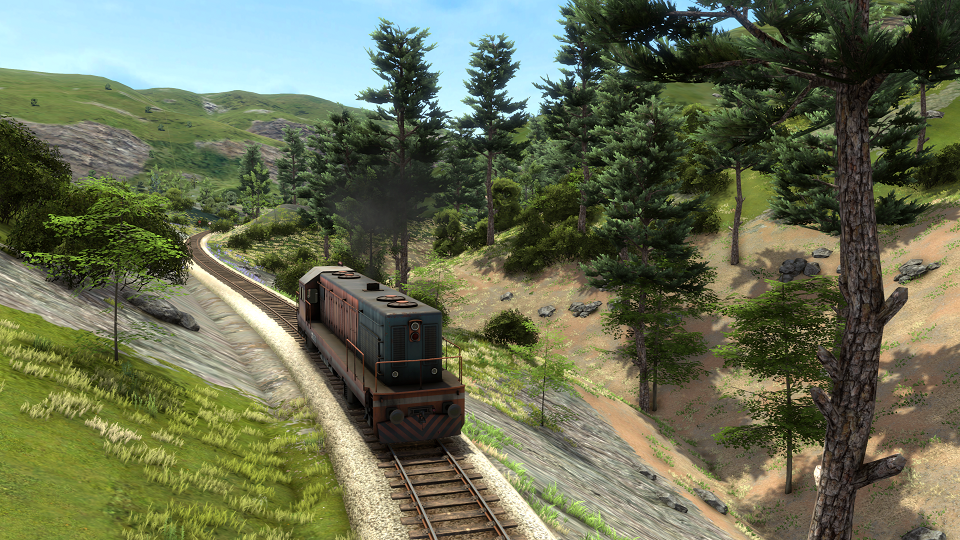
\includegraphics[width=9cm]{figures/derailvalley.png}
    %\vspace{-12pt}
    \caption{Derail Valley (Altfuture)}
\end{wrapfigure} 

Slobodan Stevic, CEO at \textit{Altfuture} and developer of \textit{Derail Valley}, explains they chose Unity “... because its VR support was better than that of other engines, back in 2016.” When asked which engine he believes is best suited for VR simulators, he adds “... it depends on the type of the simulator, its scope and style choice, as well as prior team experience.” 

\bigskip
\begin{wrapfigure}{l}{9cm}
    \vspace{12pt}
    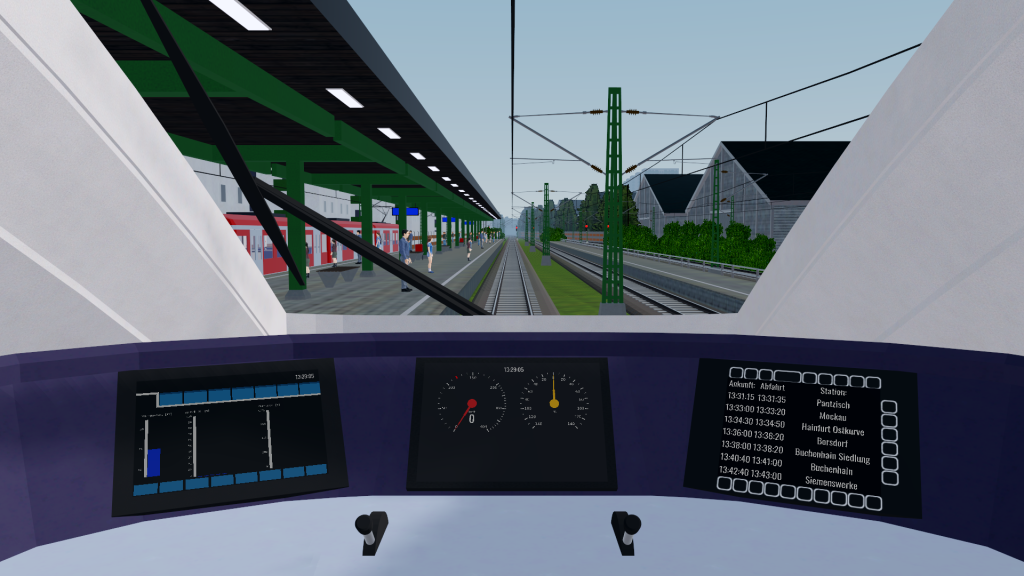
\includegraphics[width=9cm]{figures/libre_train_sim.png}
    %\vspace{-12pt}
    \caption{Libre TrainSim (GPL 3.0)}
\end{wrapfigure} 

Similarly, \textit{HaSa}, a contributor and developer of the open source project \textit{Libre TrainSim}, states that “as long as it supports `basic' requirements it is a matter of personal preference.” Describing the similarity of engine funnctioality, they also conclude that “the engine doesn't really matter.” \\[0.8cm]

Godot, the engine used to make Libre TrainSim, gets praised by HaSa for its agility. “Iteration speed is key to a good game in general. The more you iterate the better the result is.” They also comment on some downsides of the engine, claiming the renderer is “quite performance heavy out of the box which limits the creative freedom”, and the audio tools are `basic'. “We have to develop a lot of features on top to achieve good quality,” HaSa writes.

The developers we contacted behind CryEngine's small list of titles relevant to this analysis were unavailable for comment. When asking all subjects if they, in retrospect, believe their respective engine was the right choice for their game, everyone answered \textbf{yes}. 

%-----------------------------------------%

% todo
%%%                 Conclusion                  %%%
\section{Conclusion}
All engines, excluding Open 3D Engine, fulfills the Absolute Requirements (\ref{absoluterequirements}) set by Lokførerskolen. Godot and Unreal supports \texttt{gltf}-files, the most prioritized asset type. Meanwhile, CryEngine and Unity are at a disadvantage as they support fewer and less prioritized assets. While all engines require a conversion pipeline for assets, Unreal and Godot can reuse more assets out of the box. This decreases time spent on porting assets to the new engine.

The overall learning curve for the individual game engines sets Unity and Unreal engine apart from the competitors. The magnitude of the community and related quantity of available material, together with their emphasis on standards in documentation, establishes their strong position in today's game engine market. Godot is still a relatively new engine without any major titles, causing both documentation and community resources to be inadequate in quality and quantity compared to Unreal and Unity. CryEngine initially limited its use to enterprise only, resulting in less publicly available resources and documentation.

The majority of developers we reached out to advocated the choice of engine to depend on the use case of the project. As such we recommended Lokførerskolen to use Unreal Engine for their train simulator. Unreal Engine has features such as a built in dedicated spline tool which we ended up basing our whole train tracks system off, as well as dynamic occlusion culling to boost performance. It also has a one of the biggest communities among the engines analysed, as well as it is known for having photo-realistic graphics. Although finding the right solution to our problems was often an issue. We found that the community is split between using blueprints or C++, and often found that blueprints were most commonly used for beginners which slowed us down in the beginning. Since we started using blueprints first to prototype or solutions, and then later on converted it to C++ code.



%-------------------------------------------------------------------------------------------------

The \textit{jMonkeyEngine} game engine, currently in use by The Norwegian Train Driver Academy, has become primitive compared to modern technology. The importance and frequent usage of their train simulator inspire the need to migrate their software to a modern game engine. To mitigate this concern, several available solutions must be considered and evaluated.

All engines, excluding Open 3D Engine, fulfills the Absolute Requirements (\ref{absoluterequirements}) set by Lokførerskolen. Godot and Unreal supports \texttt{gltf}-files, the most prioritized asset type. Meanwhile, CryEngine and Unity are at a disadvantage as they support fewer and less prioritized assets. While all engines require a conversion pipeline for assets, Unreal and Godot can reuse more assets out of the box. This decreases time spent on porting assets to the new engine. 

The client being experienced with programming eliminates the need for GDScript as its most significant trait is being beginner-friendly. C\texttt{++}, on the other hand, may be unnecessarily advanced for the project. As for C\texttt{\#}, because of its powerful and modern functionality and versatile usage across game engines, we fail to see any relevant downsides, and we conclude it as a fitting language for the project.

The overall learning curve for the individual game engines sets Unity and Unreal engine apart from the competitors. The magnitude of the community and related quantity of available material, together with their emphasis on standards in documentation, establishes their strong position in today's game engine market. Godot is still a relatively new engine without any major titles, causing both documentation and community resources to be inadequate in quality and quantity compared to Unreal and Unity. CryEngine initially limited its use to enterprise only, resulting in less publicly available resources and documentation. 

The majority of the developers we reached out to advocated the choice of engine to heavily depend on the use case of the project. When developing an open world train simulator, this favors Unreal Engine as their engine provides tools such as dynamic occlusion culling, a dedicated spline tool and frequent release of tools used for in-house games.

In conclusion, we believe all four engines are capable of producing virtually any type of game. The difference lies in time and effort needed to achieve the same result. Throughout the analysis it is evident that Unity and Unreal Engine comes out as superior candidates, and would both be beneficial for this project. Despite Unreal Engine's steeper learning curve, we must consider the functionality provided for the specific use case of the project. Based on the results of this analysis, we conclude by proposing \textbf{Unreal Engine} to be the most suited solution for the mitigation of the current simulator.


% This here laid foundation for Requirements 
% Smooth transition to requirement specification - Henrik :D \newpage
\chapter{Requirements}

The conclusion of the game engine analysis laid the foundation for forming the requirements presented in this chapter...
% Skriv dette men bedre :)

Based on the game engine analysis, we made some requirements which is stated in this chapter

\todo{Conclude the game engine analysis - you}

The client stated their initial requirements in the form of one main goal and two sub-goals. The main goal was to create a demo which satisfied their requirements. They also presented two sub-goals, to an in-game model placing tool, and an in-game railway builder. Our requirement document are based on these requirements, but does also extends further. This chapter goes over the specific requirements set for the project by the client, the group itself, and the industry standards.


\section{Functional Requirements}

To display and visualize the core functionalities of our simulator we have chosen to utilize use cases. Use cases provides a structure and overview of the functionality works as a tool to force awareness for the requirements in the development phase. 

There was a quite unanticipated issue with defining use cases for the project as an entirety. Our main goal is, as stated previously to make a demo in the chosen engine and also make the code applicable for further development. What we discovered in the development of the demo was that the classes and structures we created often laid a groundwork for further development. We therefore decided to include two separate groups of use cases for our project. One for the application it self, and one for the use cases that got facilitated by us through development. The reasoning for including this is for the client to more easily understand the functionality and it requires us to focus on the code quality and further development perspective of the project.

\todo{sammenheng mellom use cases og issues}

\subsection{Use Case Diagram: Application}
The use case diagram illustrates all available actions for the two groups of users; students and employees. While not implied in the diagram to avoid cluttering, it should be noted that an employee has access to all functionality of the student.
\begin{figure}[H]
\centerline{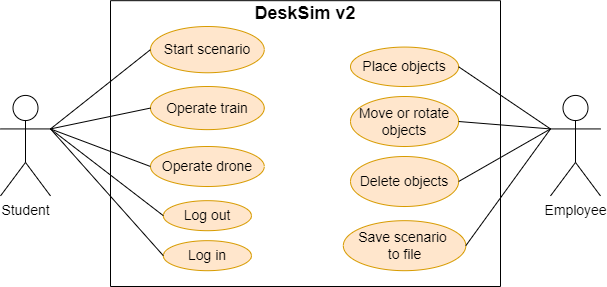
\includegraphics[width=1.0\textwidth]{figures/Desksim usecase-Final.drawio.png}}
\caption{Application use case diagram}
\label{use_case_engine}
\end{figure} 

\textbf{High Level Use Case}
% PLACE OBJECTS
\begin{table}[H]
    \centering
    \begin{tblr}{colspec={|X[.2, l]|X[.8, l]|}, hlines}
        \textbf{Use Case:} & Place objects \\
        \textbf{Actors:} & Employee \\
        \textbf{Goal:} & To place the necessary objects such as a train and a railway in a level. \\
        \textbf{Description:} & When a level is opened in editor mode the user is provided a user interface which includes a content browser. The user can click on a item in the content browser and drag it out in the level. The content browser has different categories the user can select in the top bar by clicking on the category buttons.
    \end{tblr}
    \caption{Use Case: Place objects}
\end{table}
% DELETE OBJECTS

\begin{table}[H]
    \centering
    \begin{tblr}{colspec={|X[.2, l]|X[.8, l]|}, hlines}
        \textbf{Use Case:} & Delete objects \\
        \textbf{Actors:} & Employee \\
        \textbf{Goal:} & To delete an object in the level. \\
        \textbf{Description:} & When clicking on an object in a level the user will be given the option to remove it. After the click, the user will get a trash can symbol at the top bar, next to the transformation options. After clicking on the trash can, the program will prompt the user for confirmation before permanently removing the object from the scene.
    \end{tblr}
    \caption{Use Case: Delete objects}
\end{table}

% OPERATE DRONE
\begin{table}[H]
    \centering
    \begin{tblr}{colspec={|X[.2, l]|X[.8, l]|}, hlines}
        \textbf{Use Case:} & Operate drone \\
        \textbf{Actors:} & Student \\
        \textbf{Goal:} & Maneuver the drone camera \\
        \textbf{Description:} & The student switches to drone view. This lets them move around freely in all three dimensions, forwards/backwards, horizontally, and vertically. The user can also use the mouse to freely look around in the world, and adjust the movement speed of the camera.
    \end{tblr}
    \caption{Use Case: Move or rotate objects}
\end{table}

\textbf{Low Level Use Case}

% NEW, move or rotate object
\begin{table}[H]
    \centering
    \begin{tblr}{colspec={|X[.2, l]|X[.8, l]|}, hlines}
        \textbf{Use Case:} & Move or rotate objects \\
        \textbf{Actors:} & Employee \\
        \textbf{Goal:} & To move a object or rotate it into the prosition and position you want \\
        \textbf{Precondition:} & The user has successfully opened a scenario in editor-mode \\
        \textbf{Success Scenario:} & 
        
        \todo{Skriv om - Thomas}
        
            1. The employee selects an object by clicking on it. \newline
            2. The object displays a gizmo, either in the form of arrows for moving it along each of the three-dimensional axes, or a wheel to rotate the object. \newline
            3. The user changes the mode to the one he want from the top bar icons. \newline
            
            4. \textbf{For translation:}\newline
                5. The user hovers the mouse over the arrow to select one axis, or in the middle of two arrows to select a plane. \newline
                6. The user drags the mouse to the position he wants the object to be located \newline
                
            4. \textbf{For rotation:} \newline
               5. The user presses the wheel and drags the mouse around the wheel to get the desired rotation. 
    \end{tblr}
    \caption{Use Case: Move or rotate object}
\end{table}


\begin{table}[H]
    \centering
    \begin{tblr}{colspec={|X[.2, l]|X[.8, l]|}, hlines}
        \textbf{Use Case:} & Operate Train \\
        \textbf{Actors:} & Student \\
        \textbf{Goal:} & To drive the train in a scenario \\
        \textbf{Precondition:} & The user has successfully opened a level and the levers is connected to the system through a USB port \\
        \textbf{Success Scenario:} & 
            The user accelerates or decelerates the train using the levers or the keyboard \newline
            %1. The user pushes the left lever or the keyboard to accelerate the train. \newline
            %2. The user pushes the right lever or the keyboard to apply break force on the train. \newline
            Depending on the scenario, the user has to follow some rules: \newline


                The user should not exceed the speed limit. Doing so should result in system regulated brakes turned on. \newline
                
                The user is provided information about the current speed in the Driver Machine Interface. \newline
                
                The user should follow the rules regulated by signals: \newline


                    \textbf{Main signal:} If this signal is red the user should stop. If user don't stop before the signal this should result in breaks turned on.
                    
                    \textbf{Main signal:} One green light means that the user can drive with reduced speed.
                    
                    \textbf{Main signal:} Two green lights means that the user can and should continue with the set speed.

    \end{tblr}
    \caption{Use Case: Operate Train}
\end{table}

\section{Use Case Diagram - Game engine}


\begin{figure}[H]
\centerline{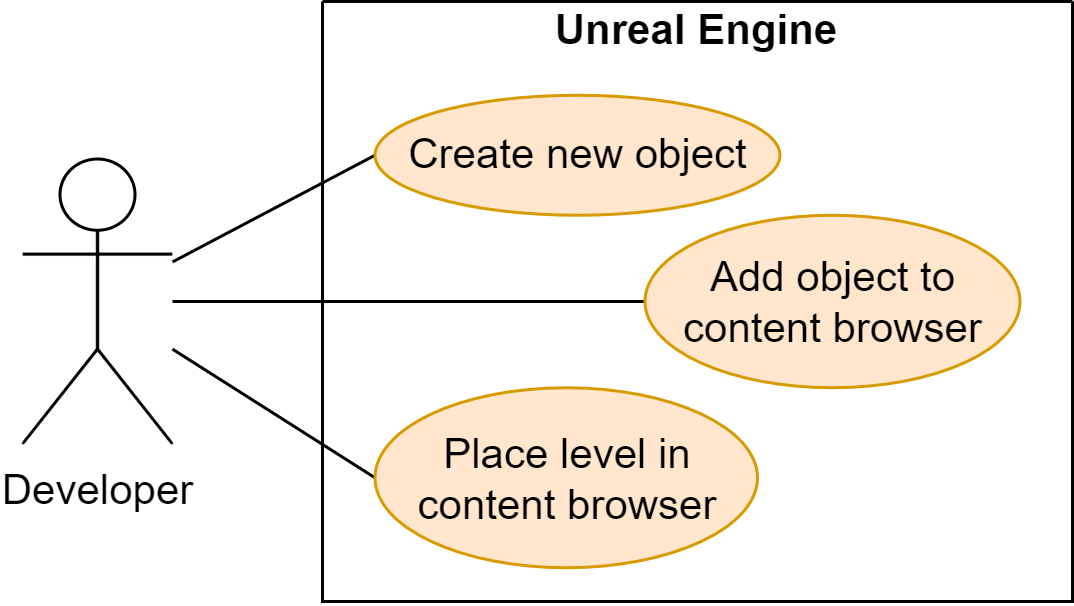
\includegraphics[width=0.9\textwidth]{figures/UEUseCase.png}}
\caption{Game Engine use case diagram}
\label{use_case_application}
\end{figure} 

\textbf{High Level Use Case}
\todo{fjern spesifikke steps og unreal objects}
\begin{table}[H]
    \centering
    \begin{tblr}{colspec={|X[.2, l]|X[.8, l]|}, hlines}
        \textbf{Use Case:} & Add Level in Main Menu \\
        \textbf{Actors:} & Developer \\
        \textbf{Goal:} & To add a level created in unreal engine to the simulator. \\
        \textbf{Description:} & When the developer has created a scene he wants to be a part of the simulator he must know the name of the level. The level name is stored as a FName, and the content browser only need its value. The FName's are immutable and case sensitive so it's important to have the right name. Open the MMObjects inside \textit{BP\_EditorHUD} blueprint located in "\textit{DeskSimV2/Source/DeskSimV2/Editor/UI}". The developer now clicks the + button to add the new level and fills in the name, description and the FName reference to the map. 
    \end{tblr}
    \caption{Use Case: Add Level in Main Menu}
\end{table}


\textbf{Low Level Use Case}


\todo{Change them from intructions to use case description}
\begin{table}[H]
    \centering
    \begin{tblr}{colspec={|X[.20, l]|X[.75, l]|}, hlines}
        \textbf{Use Case:} & Add new object \\
        \textbf{Actors:} & Developer \\
        \textbf{Goal:} & To add a new object to the game \\
        \textbf{Preconditions:} & The developer has a working version of Unreal Engine version 4.27.2 or higher. The developer has a 3D model he wants to be added in the game.  \\
        \textbf{Success Scenario:} & 

            1. The developer adds a new model to the "models" folder inside Unreal Engine \newline
            2. The developer registers the new object by deriving a new blueprint from the \cpp class relevant to the objects category.\newline
            3. The developer selects the new model as the blueprint's static mesh.\newline
            4. The blueprint is compiled and saved.\newline
            %2. The developer navigates to "C++ classes" in the content browser. \newline
            %3. The developer right clicks on either "BasicStaticObject", "Train" or "BasicSignal" or "wagon", based on what item type the object is.\newline
            %4. The developer clicks on "Derive blueprint from c++ class..." in the drop-down menu and selects the appropriate place to store the blueprint.\newline
            %5. The developer opens the blueprint and drags the imported model from step 1 into the "Static mesh" variable in the details panel for the object.\newline
            %6. The developer compiles and saves the blueprint \newline
    \end{tblr}
    \caption{Use Case: Add new object}
\end{table}
\todo{Change them from intructions to use case description}

\begin{table}[H]
    \centering
    \begin{tblr}{colspec={|X[.20, l]|X[.75, l]|}, hlines}
        \textbf{Use Case:} & Add object in Content Browser \\
        \textbf{Actors:} & Developer \\
        \textbf{Goal:} & To successfully add a created object in the content browser making it clickable and draggable in runtime.\\
        \textbf{Preconditions:} & The developer has created a new object as described in the "Add new object" use case.  \\
        \textbf{Success Scenario:} & 
        
            1. The developer opens the blueprint for the Editor-HUD.\newline
            2. The developer adds a new item to be registered as an object.\newline
            3. The developer fills in the category, name and description for the object.\newline
            4. The developer adds a reference to the actor asset.\newline
            
            It is required to close out of the application and regenerate the project files or rebuild the solution with visual studio before the object shows up in the content browser.
            %1. The developer open the \textit{BP\_EditorHUD} blueprint located in "\textit{DeskSimV2/Source/DeskSimV2/Editor/UI}". \newline
            %2. The developer clicks on the \texttt{+} icon for the CBFObjects. \newline
            %3. The developer adds the category the actor should be a part of.\newline
            %4. The developer writes a suitable name and description for the object. \newline
            %5. The developer adds the reference to the actor he wants to include.\newline
            
            %6. Close unreal engine desktop and visual studios and navigate to the file system for the project. Right-click on the \textit{DeskSimV2.uproject} files and select "generate visual studios project files" from the dropdown menu.\newline
            %7. The item should be visible and draggable in-game in the content browser. \\
        
        %\textbf{Alternative Scenario:} & 
        
            %6. Open visual studio and right click on DeskSimV2, select "rebuild" and let the solution rebuild. \newline
            %7. When its built, open DeskSimV2.uproject and check if the object is added.
    \end{tblr}
    \caption{Use Case: Add object in Content Browser}
\end{table}


\subsection{Operational Requirements}
These are the requirements which concerns the application at it's operational stage, this stage begins at the project's deadline which is the 20th of May:
\begin{itemize}
    \item The application must be able to interact with the existing Rest-API hosted by Lokførerskolen.
    \item The system must operate on Windows devices.
    \item The system must manage privileges of users and only allow elevated users to access the editor functionality.
    \item Must be transferable through a zip file
    \item The system must operate on computers which has 8GB of ram and a Intel® Core™ i5-4460 CPU or better. 
    \item Should not experience frame rate drops of lower than 60 frames per second. 
\end{itemize} 


\subsection{Security and Misuse}
\label{OperationalRequirements}
To ensure the security of the users and avoid misuse of the application the application:
\begin{itemize}
    \item must require user authentication for usage. The authentication process should be a token based system where you receive a token. The token has an expiration and should be used to authenticate the user up to its expiration. When the token expires the user will be asked to authenticate again and receive a new token. % er dette operational?
    \item should not contain bugs and/or security flaws that potentially could lead to harm or destruction of hardware components. Such flaws include bad memory handling.
    \item must not store any passwords in plain text.
\end{itemize}


\subsection{Interface Requirements}
\textbf{Menus} 
\begin{itemize}
    \item It should  be intuitive and easy for a student at Lokførerskolen to navigate the Main Menu. 
    \item The Main Menu should have the same functionality as the previous simulator and only deviate by design.
    \item All text must be available in Norwegian.
    \item Buttons should be intuitive to reduce the number of operations required for a task.
\end{itemize}

\textbf{Scenarios} 
\begin{itemize}
    \item The game should have an option to switch between a Drone Mode and a Train Mode. 
    \item The \acrshort{dmi}  viewport in a game should be responsive to the gameplay and be movable for the player.
    \item All numbers and measurements must be specified in the metric system.
\end{itemize} \newpage
\chapter{Development}

This chapter describes the work methodology and the process used during this project. We compare two agile models and describe how we implemented scrum in our group. We also review some of the sprints, by looking at the results of the sprint as well as a retrospective look.

\section{Plan}

\subsection{Development Methodology}
The choice of methodology was mainly based on these three facts: The group has little experience with game engines, the group has little to no experience on working on a project of this scale and one of the requirements of \Gls{lokforerskolen} was that they would be tightly connected to the development and emphasized this connection in their task description.

Based on the three criteria stated above, the group concluded on using an agile software development model because it allows for rapid change in these requirements. It also allows for changes in the project scope without necessarily having major impacts on releases and planned progress.

\subsection{Development model}
When choosing the optimal model for our project we looked at several different models to see if they would fit our project. Two of the development models that got evaluated was \textit{\Gls{scrum}} and \textit{\Gls{kanban}}.

\Gls{scrum} is an agile development model. It is designed for teams of ten or fewer members who divide their work into increments of work within iterations called \gls{sprint}s, which are usually between two to four weeks long.\cite{atlassian_scrum_vs_kanban} Development teams utilizing \gls{scrum} meets once a day for 15 minutes or less to assess their progress and keep everyone up to date. There are also two other meetings that are important when working with \gls{scrum}; the \gls{sprint} review, which is often held together with the project stakeholder for feedback, and a retrospective meeting to reflect on the previous \gls{sprint} results.

\Gls{kanban} is also an agile development model, which visualizes the items or tasks from start to finish, usually through a \Gls{kanban} board.\cite{kanban_2022}. The main focus for teams working with \Gls{kanban} is reducing the time a project takes from start to finish by continuously improving their workflow.

The model we chose as our development model was \Gls{scrum}. The main reason for this was that although both methodologies could be utilized and work in our project, we wanted the main focus to be creating the best simulator as possible. \Gls{scrum}, in it's nature, allows and emphasises reflection and assessment every step of the way, and has a pre-decided structure for doing so. Scrum is also the development model which is most known and used by the group previously.  

\subsection{Our implementation of \Gls{scrum}}
We aimed to use the iterative nature of \Gls{scrum} to ensure the quality of the implementation at every stage of the project, and quickly adapt to any change in the client's specifications. In the beginning of the project we had one week \gls{sprint}s and continuously discussed if we needed to increase the \gls{sprint} duration, based on the upcoming tasks. We sought out to implement \Gls{scrum} in a strict way, with daily \Gls{scrum}-meetings throughout the project.

These meetings were used as a collaborative tool to identify problems if someone was stuck, keep everyone up to speed on the project process, and create a nice work environment where we kept in touch. We believe the latter was more important than it may have seemed, because most of the work is done from home, so it was nice to keep in touch with the group at least once every day. Although these meetings are important for the group, they could occasionally be skipped if they were unnecessary. 

For managing the project, we utilized \textit{Jira} integrated with \textit{GitHub}. This integration contributed to ensuring the methodology professionalism we aimed for in the project. We used constrained and secure workflows to ensure that every issue followed the correct workflow. In simpler terms, this set the rules for how all work was to be handled throughout the project. \ref{fig:workflow} shows the direction and constraints on how an issue can progress through the different statuses.

\begin{figure}[H]
\centerline{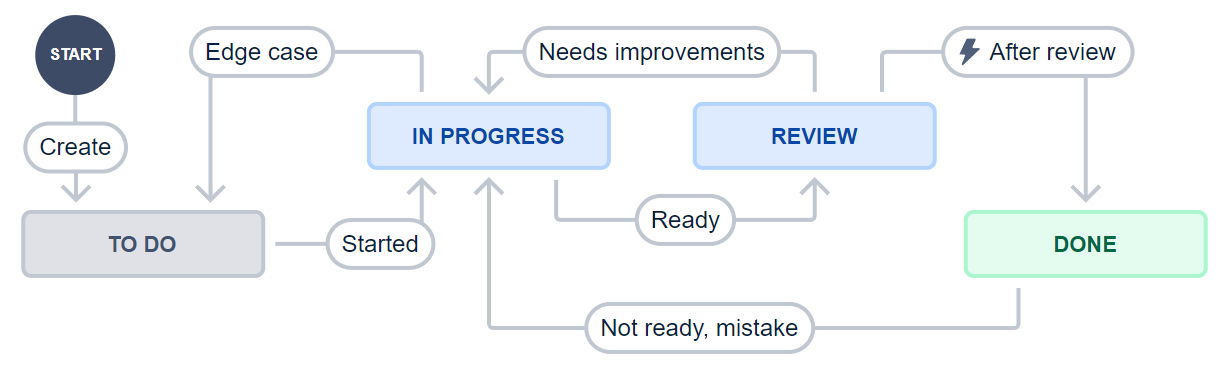
\includegraphics[width=1.0\textwidth]{figures/workflow.png}}
\caption{Issue status diagram}
\label{fig:workflow}
\end{figure} 

\subsection{Process Documentation}
\label{subsubsec:processdoc}

To log the time spent on the project, we planned to use \textit{Clockify} add-on for Jira. The add-on would allow the group to manually start a timer from within the issue in \Gls{jira}, tracking all work time until stopped. The elapsed time was manually logged along with a short comment of what was done that day. For planning the holistic overview of the project, we planned to use BigGantt. This is an extension to Jira which allows us to create a Gantt-chart in the same environment as our issues. 

\subsection{Code Documentation}

To ensure the quality and professionalism of the project we searched for and agreed upon some code conventions for \cpp programming in Unreal Engine, and standards for development. These conventions can be found in the appendix \ref{CodeConvention}. This document introduces \textit{Doxygen}, a documentation generator we utilized for automatically producing code documentation for the client. We saw this as a necessity, especially because we were writing code for a client. To do this, we had to follow Doxygen's documentation standard when commenting code. When the development came to a conclusion, we generated a folder of HTML-files, which can be hosted as a website to display the documentation. It is located inside the \verb|/Documentation|-folder in the project repository. 


\begin{figure}[H]
\centerline{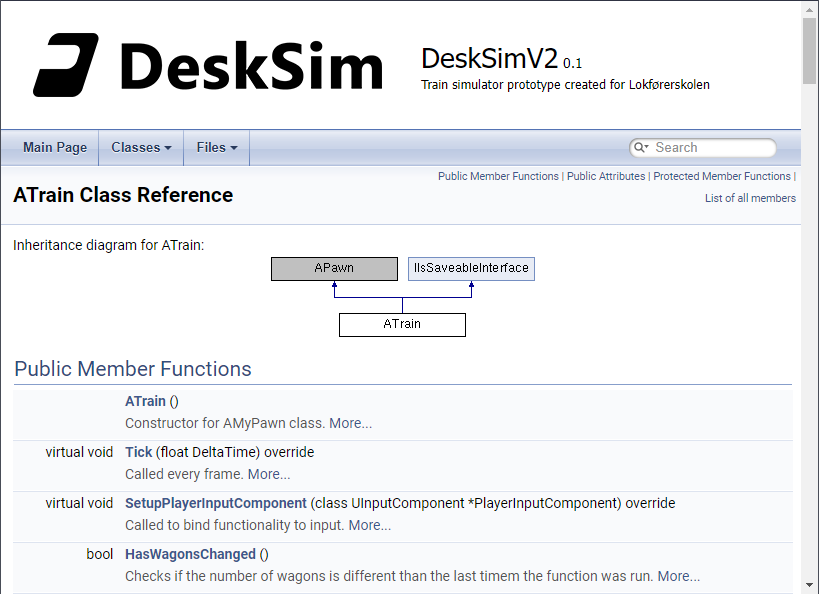
\includegraphics[width=1.0\textwidth]{figures/Documentation1.png}}
\caption{The documentation page for the ATrain class}
\label{fig:Documentation1}
\end{figure} 

The documentation contains all files, classes, functions and variables used in the project, and presents the user with menus, lists and a search bar for easy navigation. As shown in \ref{Documentation1}, a class page displays all relevant information for a class. Figure \ref{Documentation2} is captured further down on the same page, showing an example for a member function description. 

\begin{figure}[H]
\centerline{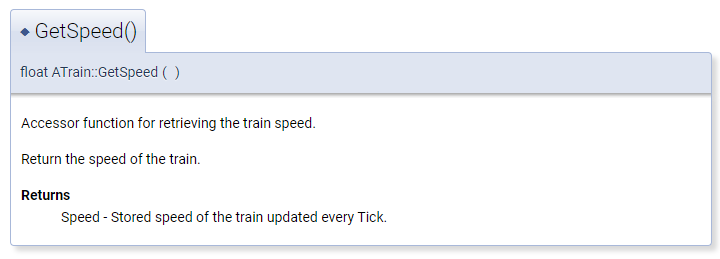
\includegraphics[width=1.0\textwidth]{figures/Documentation2.png}}
\caption{The documentation for ATrain member function GetSpeed}
\label{Documentation2}
\end{figure} 

\subsection{Git Workflow}
The group agreed upon some rules for working with git. these rules were made to ensure that the code was well protected against human error. The workflow consists of seven rules and it is mandatory for all group members to follow.

\begin{itemize}
\item Always create a new branch when starting work on a feature. No work should be done directly on the main branch.
\item This is, and should be the naming convention for branches: \\
\verb|<issue_number>-<branch_name>|
\item This is, and should be the only commit convention: \\
\verb|[#<issue-number>]-<description>|
\item When the work is completed on a branch, it must be deleted after the work is merged into the main branch.
\item Code should be committed often, either when a task is finished or the newly written code is fully functional.
\item Do not commit code that doesn't compile. Code should be tested before it is committed.
\item When a feature is complete, its branch should be merged into the current milestone branch. When the work for one milestone is completed, this branch should be merged with main. % Your own branch?



\end{itemize} 

\todo{config?? hmm. kopier noe fra prosjektplanen om git workflow}


\subsection{Gantt Chart}

Figure \ref{gannt_chart} presents the milestones for the project and their planned time schedule. This chart is a visualization of the planned project process, and it will be compared to the actual project process in \ref{deviation_process}. % Kanskje linke til en større versjon i appendices?

\begin{figure}[H]
\centerline{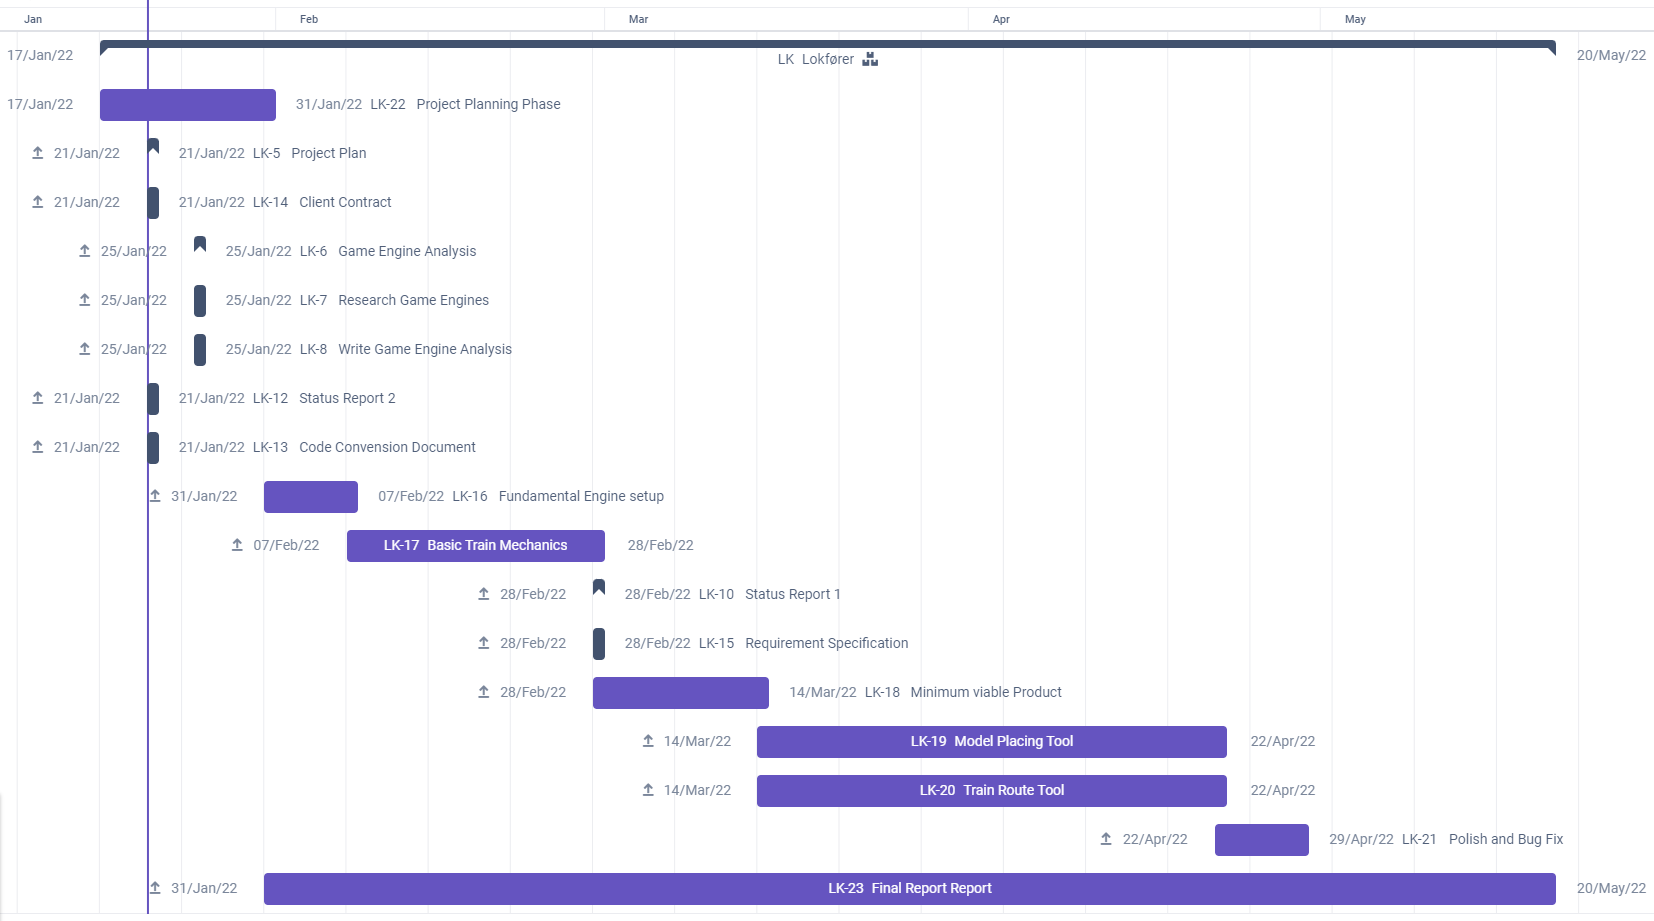
\includegraphics[width=1.0\textwidth]{figures/Gantt.png}}
\caption{Gantt chart}
\label{gannt_chart}
\end{figure} 



\begin{comment}
This chapter will provide a detailed description the methodology, and how we used it. It will describe some of our sprints and the project process as an entirety. There will also be a graphical view of the sprints showing the progress, and explanations over changes in the project scope.
\end{comment}



\section{Process}

This section will describe our usage of development tools such as \Gls{jira}. It will also cover the estimation process, examples of weekly \glspl{sprint} and a overview over the changes and deviation from the original project plan.

\subsection{\Gls{jira}}

The group used \Gls{jira} for implementing scrum into our project. We created our product backlog and kept track over all issues and \glspl{sprint} in the software. To use Jira to the full extent we had to follow the git workflow. When a push was made to GitHub, using the correct commit conventions provided a commit history available in the software. 

\begin{figure}[H]
\centerline{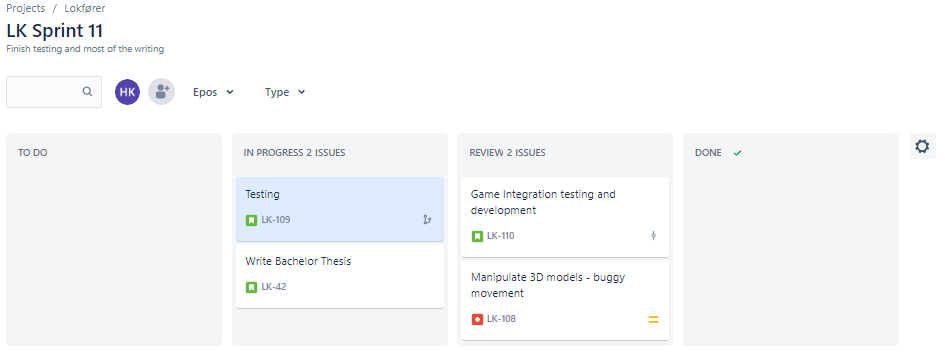
\includegraphics[width=1.0\textwidth]{figures/Jira_scrum board.PNG}}
\caption{Scrum board in Jira Software}
\label{gannt_chart}
\end{figure} 


\subsection{Sprints}
Our project consisted of eleven sprints. Figure \ref{sprint_overview_img}, contains a visualization of the main focus area for each of the sprints. Sprint three, seven and eleven is displayed below to give an example of how the group approached and solved issues related to setting up, developing and testing the system. For each of the sprint's a table is displayed to show the result of the sprint with the estimations made.


\begin{figure}[H]
    \centering
    \vspace{12pt}
    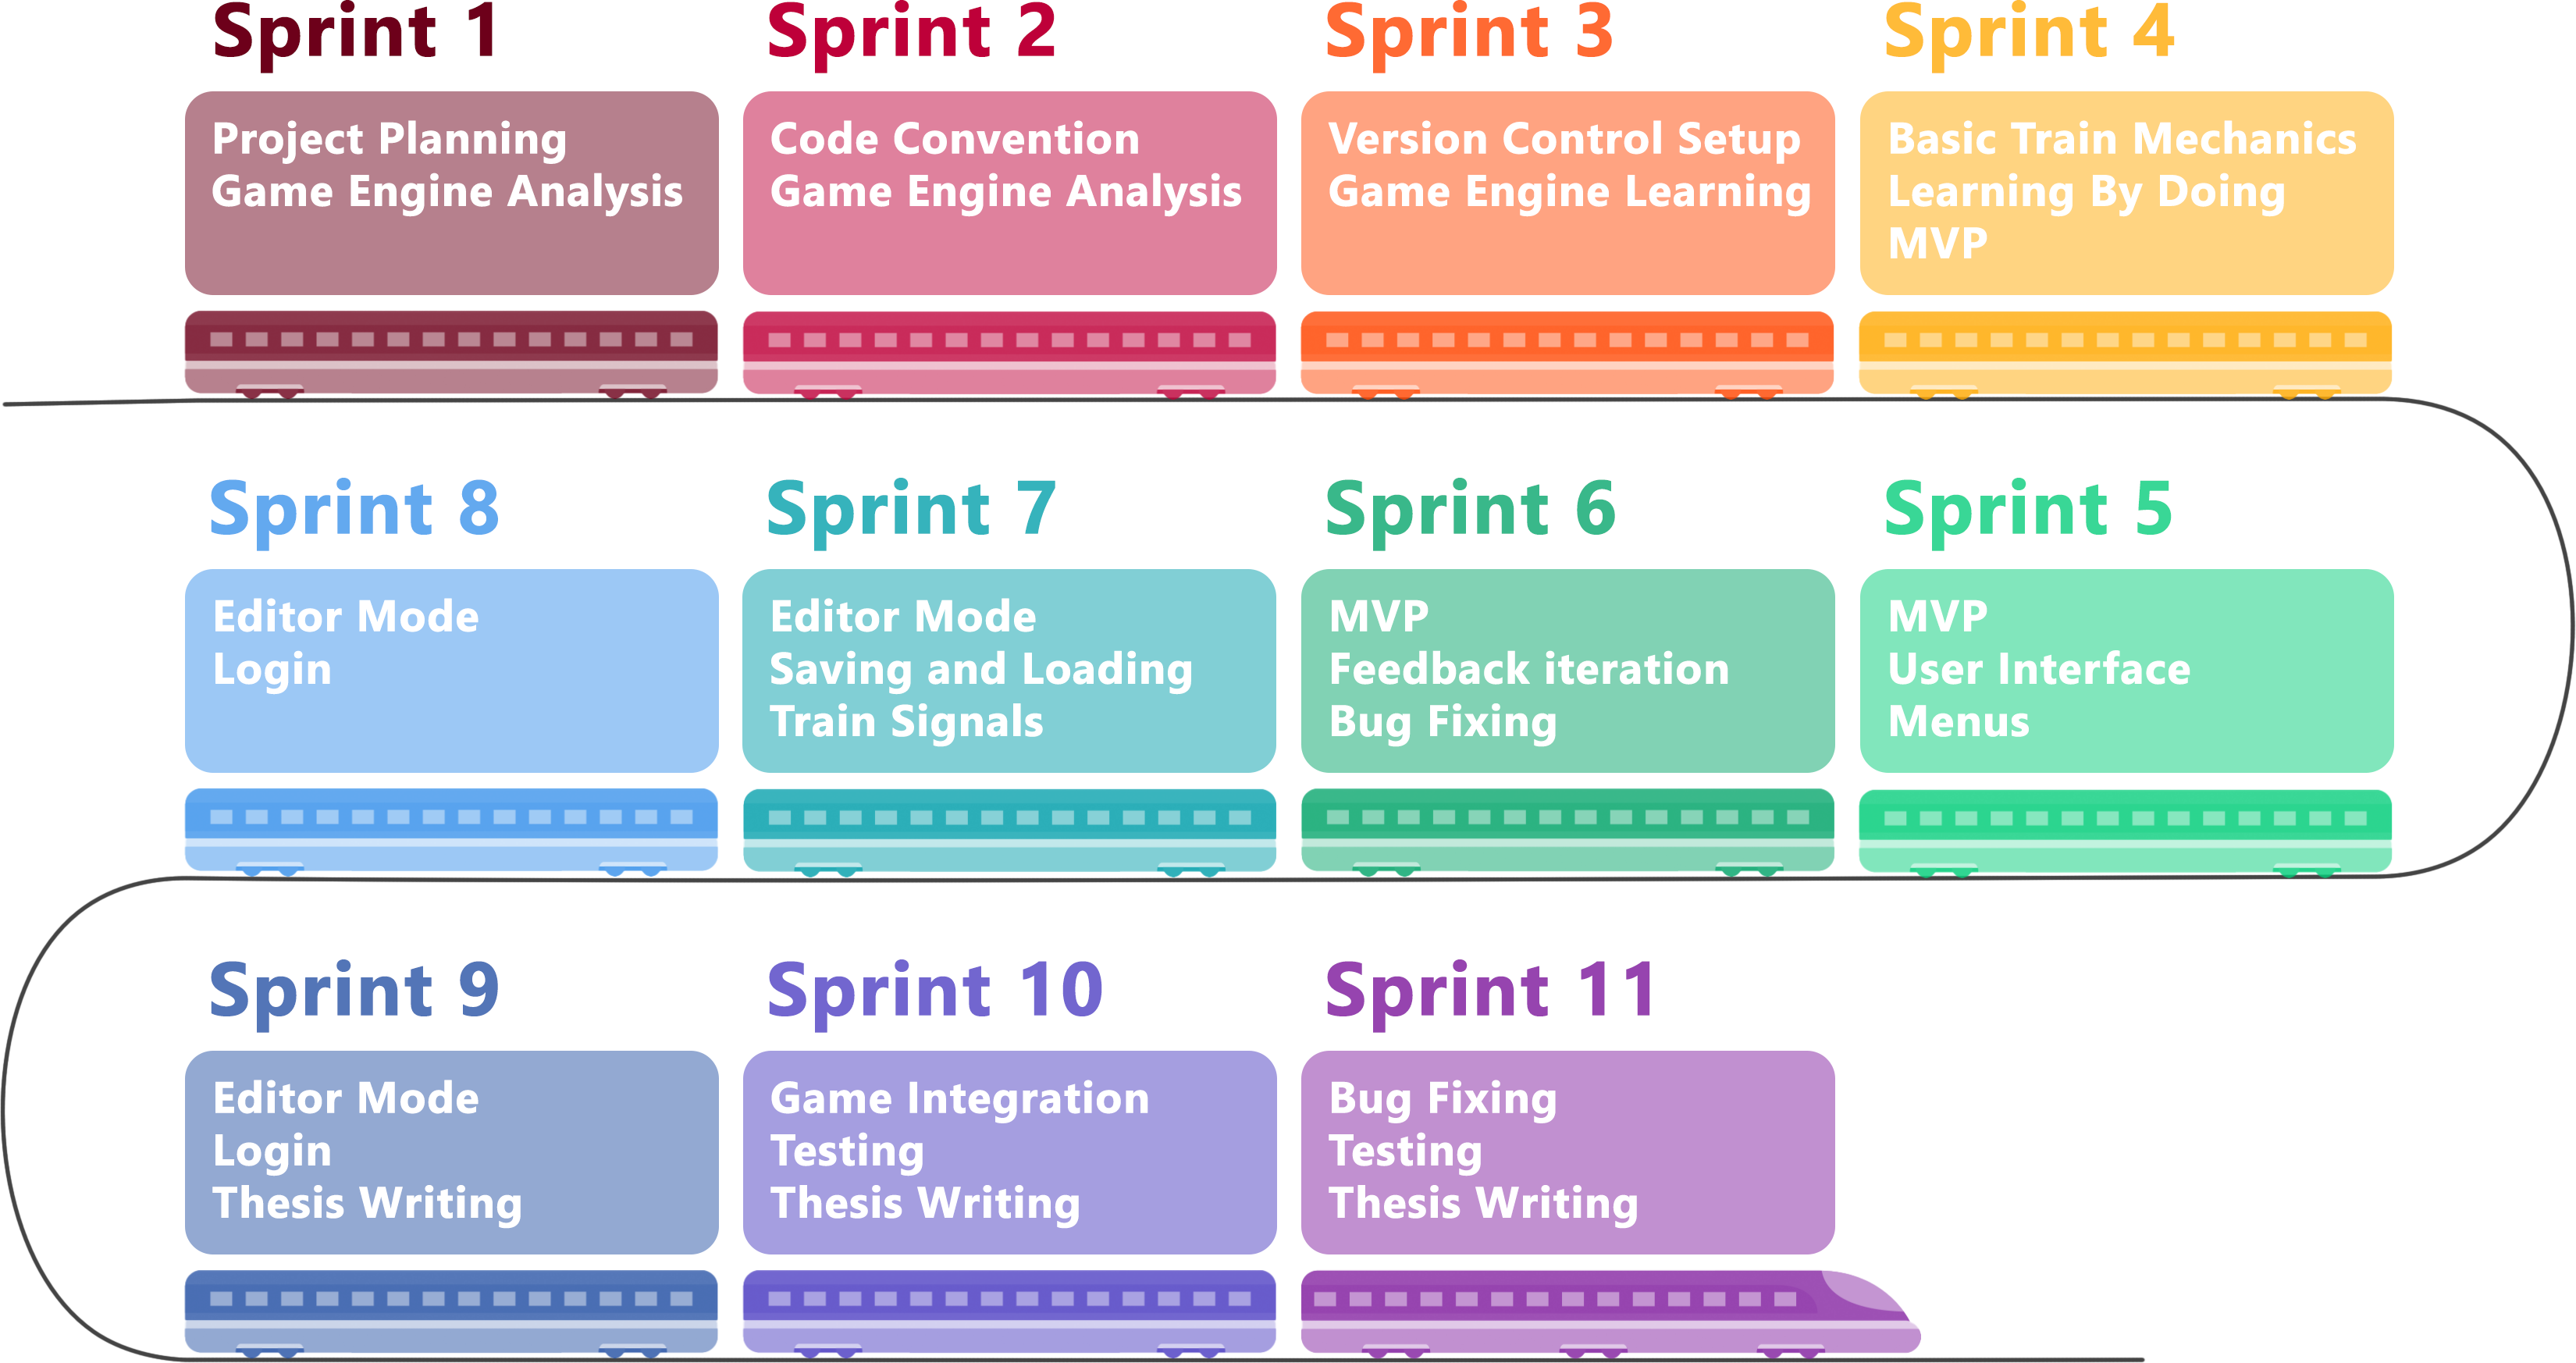
\includegraphics[width=\textwidth]{figures/SprintModel.png}
    %\vspace{-12pt}
    \caption{Overview of all sprints}
    \label{sprint_overview_img}
\end{figure} 

The sprint meeting notes are written with three different sections. A section about the Goals we have for the sprint. A section which discusses the result of the sprint. And a retrospective section where we will discuss and reflect on the result of the sprint with the goals in mind. 

\textbf{Estimations} \\
We started out estimating issues in T-shirt sizes, ranging from 1-4 which imitates small, medium, large and extra large issues. After sprint 3 we decided to change the estimation strategy to hopefully estimate more accurately. We changed the estimations to be an exact number, but tried to keep the task sizes low.

\textbf{Statuses} \\
The issues can be set to one of five statuses describing its current state in a sprint. The statuses are: \\
\textbf{Wishlist} - The issues that is taken out of the project scope and in to a list of functionality that we can decide to include if we have time later in the project. \\
\textbf{To Do} - This are the section for issues that are waiting to be developed. \\
\textbf{In Progress} - The issues that are currently being developed.
\textbf{Review} - The issues that is currently under review by peers.
\\
\textbf{Done} - The issues that has been completed in the sprint.\\

\begin{large}
    \textbf{Sprint 3} \\
\end{large}
\textbf{Date:} 07.02.2022 \\ 
\textbf{Present:} Endre, Henrik, John Ole and Thomas \\
\textbf{Period:} 07.02 - 14.02 \\ 

\textbf{Sprint Goal:}
\begin{itemize}
    \item Review and deliver Game Engine Analysis to the client and to our supervisor
    \item Integrate Jira with GitHub
    \item Setup the repository in GitHub with an Unreal project
\end{itemize}

\textbf{Sprint result:} \\
“This is the first sprint where we managed to get all our goals finished in time. We managed to finish the setup and integration with Jira on time, which resulted in being able finish the MVP within two weeks.”

%This is the first sprint that we actually managed to get all our goals finished in
%time. We managed to finish the setup and integration with Jira and this results
%in a decrease of time delay from our original plan to be finished with the MVP in
%two week
%a decrease of time delay from our original plan to be finished with the MVP within two weeks. \todo{siste setningen her ??}

\begin{table}[H]
    \centering
    \begin{tblr}{
      colspec={|X[0.20, l]|X[0.30, l]|X[0.50, l]|}, hlines,
      column{1} = {gray9},
      column{2} = {purple9},,
      column{3} = {green9},
      row{2} = {c}
    }
    \SetCell{bg=gray4}  & \textbf{Other statuses} & \textbf{Done} \\
        Issues & - & \SetCell[c=1]{l}  Write Engine Analysis \newline\newline Integrate GitHub and Jira \newline\newline Setup Repository \newline\newline Code Convension Document \newline\newline Learning Engine Basics \\
        Estimates & \SetCell[c=1]{c} 0 & \SetCell[c=1]{c} 4 + 2 + 2 + 2 + 2
    \end{tblr}
     \caption{Overview of issue status at the end of sprint 3}
\end{table}

\textbf{Retrospective:} \\
“We finished all the tasks we had in mind and also managed to start learning the engine basics as well. This means that we from next week can start working towards the MVP. We discussed increasing the sprint length from one to two weeks for the next sprint, but decided to keep the one week sprint because we want to have a new retrospective meeting next week and evaluate the accuracy of the story point estimates we made on the issues regarding the MVP to figure out if we can finish the MVP in the allocated time. This decision was made because the time we have set to be finished with the MVP and display it to the client is the 14th of March.”


\begin{large}
    \textbf{Sprint 7} \\
\end{large}
\textbf{Date:} 07.03.2022 \\ 
\textbf{Present:} Endre, Henrik, John Ole and Thomas \\
\textbf{Period:} 07.03 - 21.03 \\ 

\textbf{Sprint Goal:}
\begin{itemize}
    \item Finish first draft of requirement specification and status report 1.
    \item Finish the MVP scenario
\end{itemize}

\textbf{Sprint result:} \\
“The MVP got finished and put together. We had some issues with the environment creation and it's time consumption, but the estimations we made for three environment creation tasks was more accurate than our previous estimations. All the necessary functionality was there to display the MVP to the client except the basic statuses which we only controlled by a timer instead of an controller. The basic statuses was only missing a few hours of work and is therefore almost finished.”

\begin{table}[H]
    \centering
    \begin{tblr}{
      colspec={|X[0.15, c]|X[0.21, c]|X[0.21, c]|X[0.21, c]|X[0.22, c]|}, hlines,
      column{1} = {gray9},
      column{2} = {purple9},
      column{3} = {blue9},
      column{4} = {blue9},
      column{5} = {green9},
    }
    \SetCell{bg=gray4}  &
    \textbf{Wishlist} &
    \textbf{To do} &
    \textbf{In Progress} &
    \textbf{Done} \\
        Issues 
        & \SetCell[c=1]{l} Editor mode: \newline - Generate flat terrain (14) \newline - Manipulate terrain (20) \newline - Dynamic buttons (10)
        & \SetCell[c=1]{l} Place and edit railway (28) \newline \newline Load scenario from file (14) \newline \newline Save scenario to file (14) Static Buttons on screen (7)
        & \SetCell[c=1]{l} Main Goal: \newline - Signal Controller (21) \newline - Emergency Breaks (7) \newline - Stop Scenario (21) \newline \newline In game content browser (25) \newline \newline Save Object to File (20) \newline \newline Load Object From File (20)
        & \SetCell[c=1]{l} Main Menu (14) \newline \newline Basic Statuses (7) \newline \newline Second iteration Requirement Specification (21)  \newline \newline Place 3D Models (12) \newline \newline Manipulate 3D Models (25)  \\
        Estimates & 44 & 63 & 114 & 79
    \end{tblr}
     \caption{Overview of issue status at the end of sprint 7}
\end{table}


\textbf{Retrospective:} \\
“The sprint goals was achieved, but the basic statuses was only implemented to work with the MVP scenario and not finished to he extent we want in the final product. We want the signals to be controlled by a controller and be able to trigger events. New issues for this will come in the next sprint. We finished 93 work hours in the sprint and we feel that our estimations on the different tasks are beginning to get better and more accurate to how we progress in the sprints.”

\begin{large}
    \textbf{Sprint 10} \\
\end{large}
\textbf{Date:} 21.02.2022 \\ 
\textbf{Present:} Endre, Henrik, John Ole and Thomas \\
\textbf{Period:} 18.04 - 01.05 \\ 

\textbf{Sprint Goal:}
\begin{itemize}
    \item Finish the demo test level
    \item Have the simulator ready for testing (all functionality ready)
\end{itemize}

\textbf{Sprint result:} \\
“We finished the demo test level and got the simulator ready for the student tests. The process was challenging because it was important that the quality was ensured because the simulator is going to be tested on students from Lokførerskolen next Monday.”

\begin{table}[H]
    \centering
    \begin{tblr}{
      colspec={|X[0.15, c]|X[0.28, c]|X[0.28, c]|X[0.29, c]|}, hlines,
      column{1} = {gray9},
      column{2} = {purple9},
      column{3} = {blue9},
      column{4} = {green9},
    }
    \SetCell{bg=gray4}  &
    \textbf{Wishlist} &
    \textbf{In Progress} &
    \textbf{Done} \\
        Issues 
        & \SetCell[c=1]{l} Place and Edit Railways (28) 
        & \SetCell[c=1]{l} Write bachelor Thesis (30) \newline \newline Game integration testing (30)
        & \SetCell[c=1]{l} Basic Train cars (10) \newline \newline Convert in-game menu to c++ (4) \newline \newline Demo Test Level: \newline - Create Environment (4) \newline - Add train and wagon (1) \newline Add signal and triggerboxes (2) \newline - Add railway (2) \newline - Add station (1) \newline - Possesion switch between drone and train (2) \newline Fix camera possesion bug (4) \newline \newline Delete editor objects (5) \\
        Estimates & 28 & 60 & 21
    \end{tblr}
     \caption{Overview of issue status at the end of sprint 8}
\end{table}


\textbf{Retrospective:}

“Even though we only finished 21 of the story point estimates, we have spent much time on writing the final thesis. All tasks we set out to do is finished except the Place and edit railway issue which got excluded from the project scope. This particular task was taking up a lot of development time due to the unforeseen difficulty of the task. After discussing internally and with the client, we concluded that all the functionality we were developing in the in-game editor mode were reflections of what offers in-engine. This made a hindrance to further development of editor functionality, which was then removed from the project, as the client agreed that it would be easier to utilize Unreal Engine itself for this functionality.

When planning the sprint we added an issue for game integration testing. This issue would contain all the bugs, errors and code mistakes we could find when trying to build and package the game. Since the scope of the issue increases when working on it, we decided to not include as much issues to this sprint to ensure that this issue gets the attention it needs.”

%%%%%%%%%%%%%%%%%%%%%%%%%%%%%%%%%%%% SCRUM %%%%%%%%%%%%%%%%%%%%%%%%%%%%%%%%%%%%%%%%%%

\subsection{Deviation from original plan} \label{deviation_process}
While developing the simulator we encountered some situations where we decided to or were forced to deviate from our original plan. This section will explain the main deviations, and they will be addressed further in the discussion \todo{reference discussion}  

\subsubsection{Deviations in project process plan}
Figure \ref{Epic_comparison_img} shows the milestones for the project with it's allocated time period. There were some deviations in the project process compared to what we planned in the beginning of the project. As the figure shows our planned progress was fairly similar to the planned process, but it was some delays in the beginning of the project. some milestones was being worked on in the same time such as basic train mechanics and minimum viable project. There was also a new milestone (Testing and Game Integration) we did not expect was going to take up as much time as it did.

\subsubsection{Deviation in estimation process}

As previously stated the estimations was done in T-Shirt sized estimations. We did not find these estimations valuable when working with scrum. Further estimations did not get easier after reviewing the T-shirt sized issues because it had margins such as 1-3 hours, 1 day and 2-3 days. We wanted to change it to get an exact value we could utilize to set better and more realistic estimations.

\begin{figure}[H]
    \centering
    \vspace{12pt}
    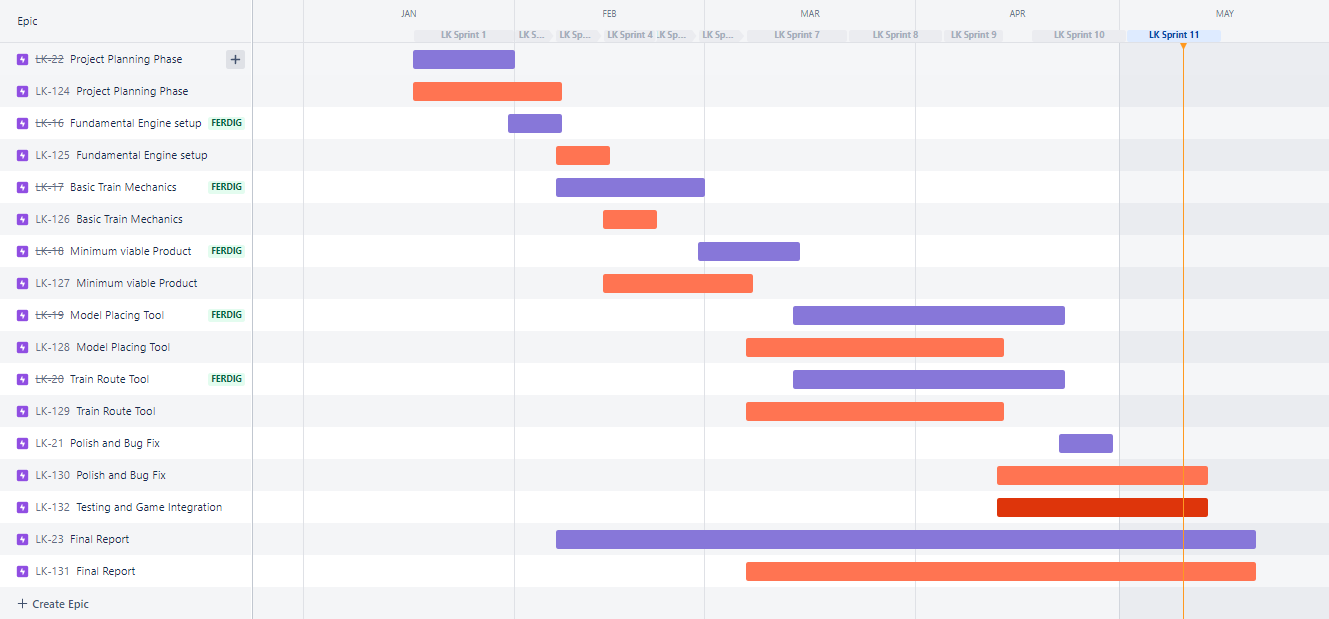
\includegraphics[width=12cm]{figures/Jira comparisoncroped.png}
    \caption{Comparison of original project plan (purple), to the actual project process (orange). The red bar shows an epic in the development we did not plan for but that was necessary to include}
    \label{Epic_comparison_img}
\end{figure} 

\subsubsection{Daily scrum meetings}

The daily scrum meeting worked well in the beginning of the project. We were all sharing our experiences and letting the group know what we had done the previous day and making sure everyone know the current status of the project. After one month of the development process these meeting began to feel forced and not very productive, they often went way over the time limit and noting them down just seemed like a waste of time. We therefore decided to stop doing these meeting as a forced, structural procedure. We did not stop having the meetings but we only noted them down when there was any relevant information that needed to be addressed later in the development which had not been addressed in the retrospective meetings.

\subsubsection{Sprint lengths}

We started the project with a sprint length of one week. After sprint 6 we decided to increase the length to two weeks because of the increase of magnitude in the upcoming milestones with was the model placing and train route tool. This decision was made as previously stated in the retrospective for week 6 to produce more functionality and give our self more time to produce code before evaluating it. The rapid time between development and planning also became more an obstacle than a benefit for us as it began to halt the process by only allowing us to finish small sections of the functionality at a time.

% Disse kan egt splittes opp, så ^denne er her, og vdenne er i discussion

The change in the sprint length also provided us with the opportunity to take a rest day or a research day. This day was allocated at the beginning of each sprint after sprint 7. This day was voluntary for each member of the group and the different group members used the day differently. Some used it to continue working on the previous sprint, some used it to write about the implementations they had done in the previous sprint, and some took an extra day of rest.
 \newpage
\chapter{Technical Design}

This chapter describes the design and choices behind the technological systems which lay the foundation for the application. The development environment is based around Unreal Engine and \cpp.

\section{System Architecture}

The code architecture is based around the object-oriented nature of \cpp and patterns within game programming. Limited by the development environment, we had to implement all classes as derivatives from Unreal Engine's base classes. These classes enable common functionality such as rendering, collisions and mathematical operations such as translation and rotation. We continued this style of inheritance, defining base properties for objects, and deriving further into special classes if needed. A prime example of this is in the editor mode of the application, where each object in a level is treated as an \textit{EditorObject}, including trains and railways. An \textit{EditorObject} is an interactable entity in a level. These can be manipulated by the \textit{EditorController}, which handles all user input and level manipulation.

\section{Application module Architecture}
The application's hierarchy has been divided into four figures for clarity. The model's shows all the actors, pawns, widgets, etc, and tries to visualize their inter-connectivity in the system.

Figure \ref{LoginHierFigure} shows the different game modes a level can open as and what HUD is used for the game modes. Both game mode and HUD will be explained in more detail in \ref{implementation_chapter} and \ref{HUD_implementation} respectively.

\begin{figure}[H]
    \centerline{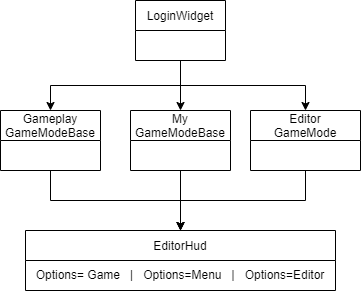
\includegraphics[width=0.6\textwidth]{figures/Untitled Diagram-Login.drawio.png}}
    \caption[Hierarchy of application start up functionality ]{ }
    \label{LoginHierFigure}
\end{figure} 

To decide what HUD elements should be displayed, an Options string is sent with the new game mode. This string could either be blank, which defaults to Menu, "Game" to start a level in simulating mode or "Editor" to start the level in editor mode. The three next figures displays the hierarchy of these three gamemodes respectively.
\begin{figure}[H]
    \centerline{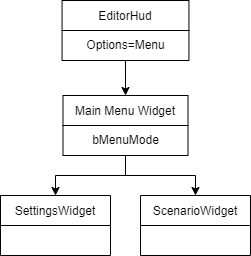
\includegraphics[width=0.5\textwidth]{figures/Untitled Diagram-Main Menu.drawio.png}}
    \caption[Hierarchy of application start up functionality ]{The module hierarchy for main menu mode }
    \label{fig::menu_hierarcy}
\end{figure} 

\begin{figure}[H]
\centering
\begin{minipage}{.5\textwidth}
  \centering
  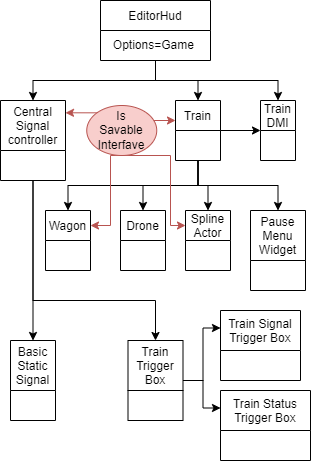
\includegraphics[width=0.95\linewidth]{figures/Untitled Diagram-Game.drawio.png}
  \captionof{figure}{The module hierarchy for simulating mode}
  \label{fig:sim_mode}
\end{minipage}%
\begin{minipage}{.5\textwidth}
  \centering
  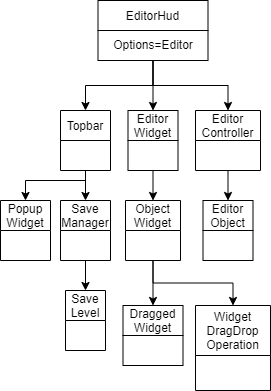
\includegraphics[width=0.95\linewidth]{figures/Untitled Diagram-Editor.drawio.png}
  \captionof{figure}{The module hierarchy for editor mode}
  \label{fig:editor_mode}
\end{minipage}
\end{figure}





\section{Network Architecture}

Authentication is currently the only system which uses the network. While multiplayer is a feature used in the existing \gls{desksim} solution, it is not a part of this demo. 

User authentication is done using the existing solution in use at Lokførerskolen. Their system uses two endpoints, the first receives a username and password and returns a JWT (JSON Web Token) on success. The JWT is then sent to the second endpoint, which returns a JSON UserObject which contains info such as ID, Username, Roles, etc. 

When the program is launched a login screen is presented to the user, where a username and password must be entered. The user must be authenticated in order to use the software. If an error such as invalid username or password, or an error with the server occurs, an error message is shown to the user. Once the user is authenticated their info is stored for the duration of the session. The user-info is never stored to any file, which means the user needs to log in each time the program is started. Because the username, password nor token is ever stored locally, they cannot be extracted from local files in order to obtain private credentials.


%\vspace*{1 cm} %Temporary fix for tables going into eachother
\begin{figure}[H]
    \centerline{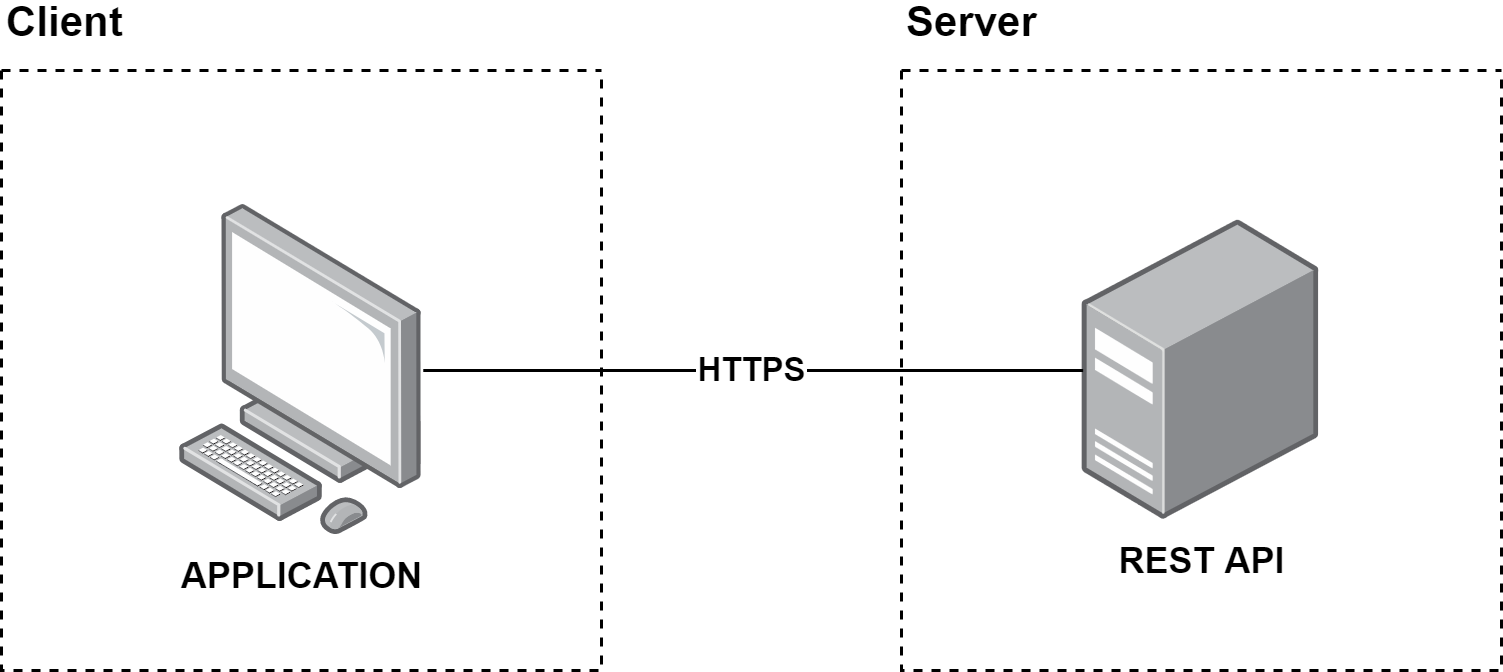
\includegraphics[width=0.9\textwidth]{figures/NetworkArchitecture.png}}
    \caption{A diagram for the network architecture}
\end{figure} 

\subsection{File Structure}
Unreal Engine separates files into two main folders, \verb|Source| for code files and \verb|Content| for asset files. We decided to structure the code files into folders based on their area of use in the context of the software. All other asset files were separated based on their type inside the \verb|Content|-folder.


\begin{figure}[h]
    \centering
    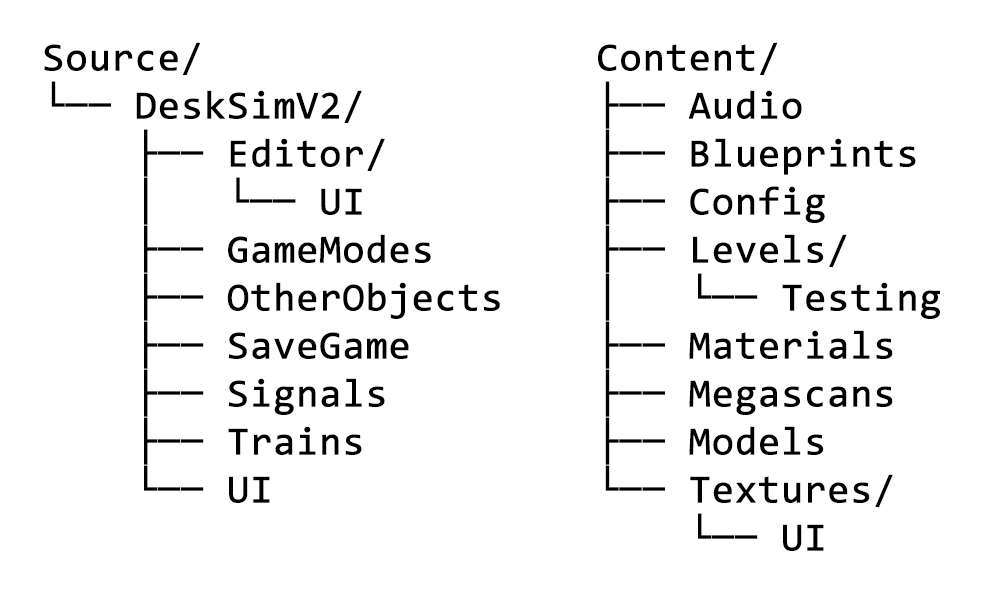
\includegraphics[width=0.75\textwidth]{figures/Files3.png}
    %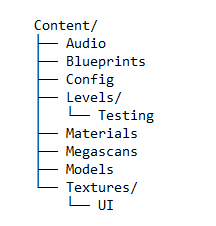
\includegraphics[width=0.4\textwidth]{figures/Files2.png}
    %\vspace{-12pt}
    \caption{File hierarchy for Source and Content}
    \label{Stop_Signal_img}
\end{figure} 


%\subsubsection{Scenarios}
% System
%\subsection{Design choices}
% 

% Have to figure out what to include in this section!
 \newpage
\chapter{Product Overview}

% did the ui meet the interface requirements?
% fill inn text inbetween images
% 
% iterate on text and images

% Frempek???
This chapter describes the product as seen from a user's perspective. It focuses on giving a holistic understanding of the simulator to provide context for further chapters. DeskSim v2 as a product is a functional simulator and a building tool for the simulator. The following section will provide a representation of both the simulator and the building tool, as well as how they are presented to the user. All texts and buttons are represented in Norwegian. 

\section{Menus}

When the application is started the log in screen displays a basic user interface where the user will enter their credentials to log in and gain access to the simulator. You must be an authenticated user to use the application, since no guest mode exists. If there is an error when logging in, such as an empty field or wrong username and password, a small error text will be displayed to the user. 

\begin{figure}[H]
    \centering
    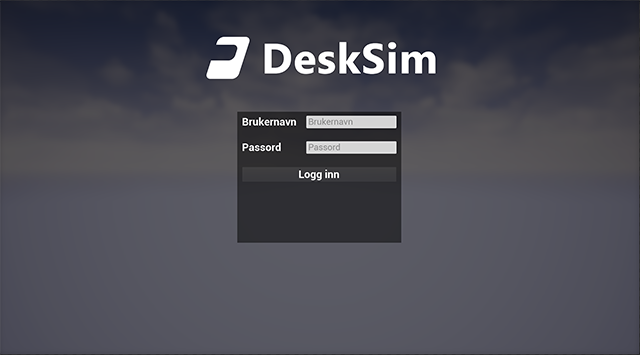
\includegraphics[width=0.8\textwidth]{figures/LogIn1.PNG}
    \caption{DeskSimV2: Log in screen}
    \label{Log_in_menu_img}
\end{figure} 


The main menu allows the user to select the level/scenario they want to run. These scenarios are separated into main categories displayed as tabs. The categories are based on the ones Lokførerskolen uses today. If the user has admin or teacher privileges they have the option to start a level/scenario in editing mode as well, as is shown with the "Editor" button in figure \ref{Main_Menu_img}.

\begin{figure}[H]
    \centering
    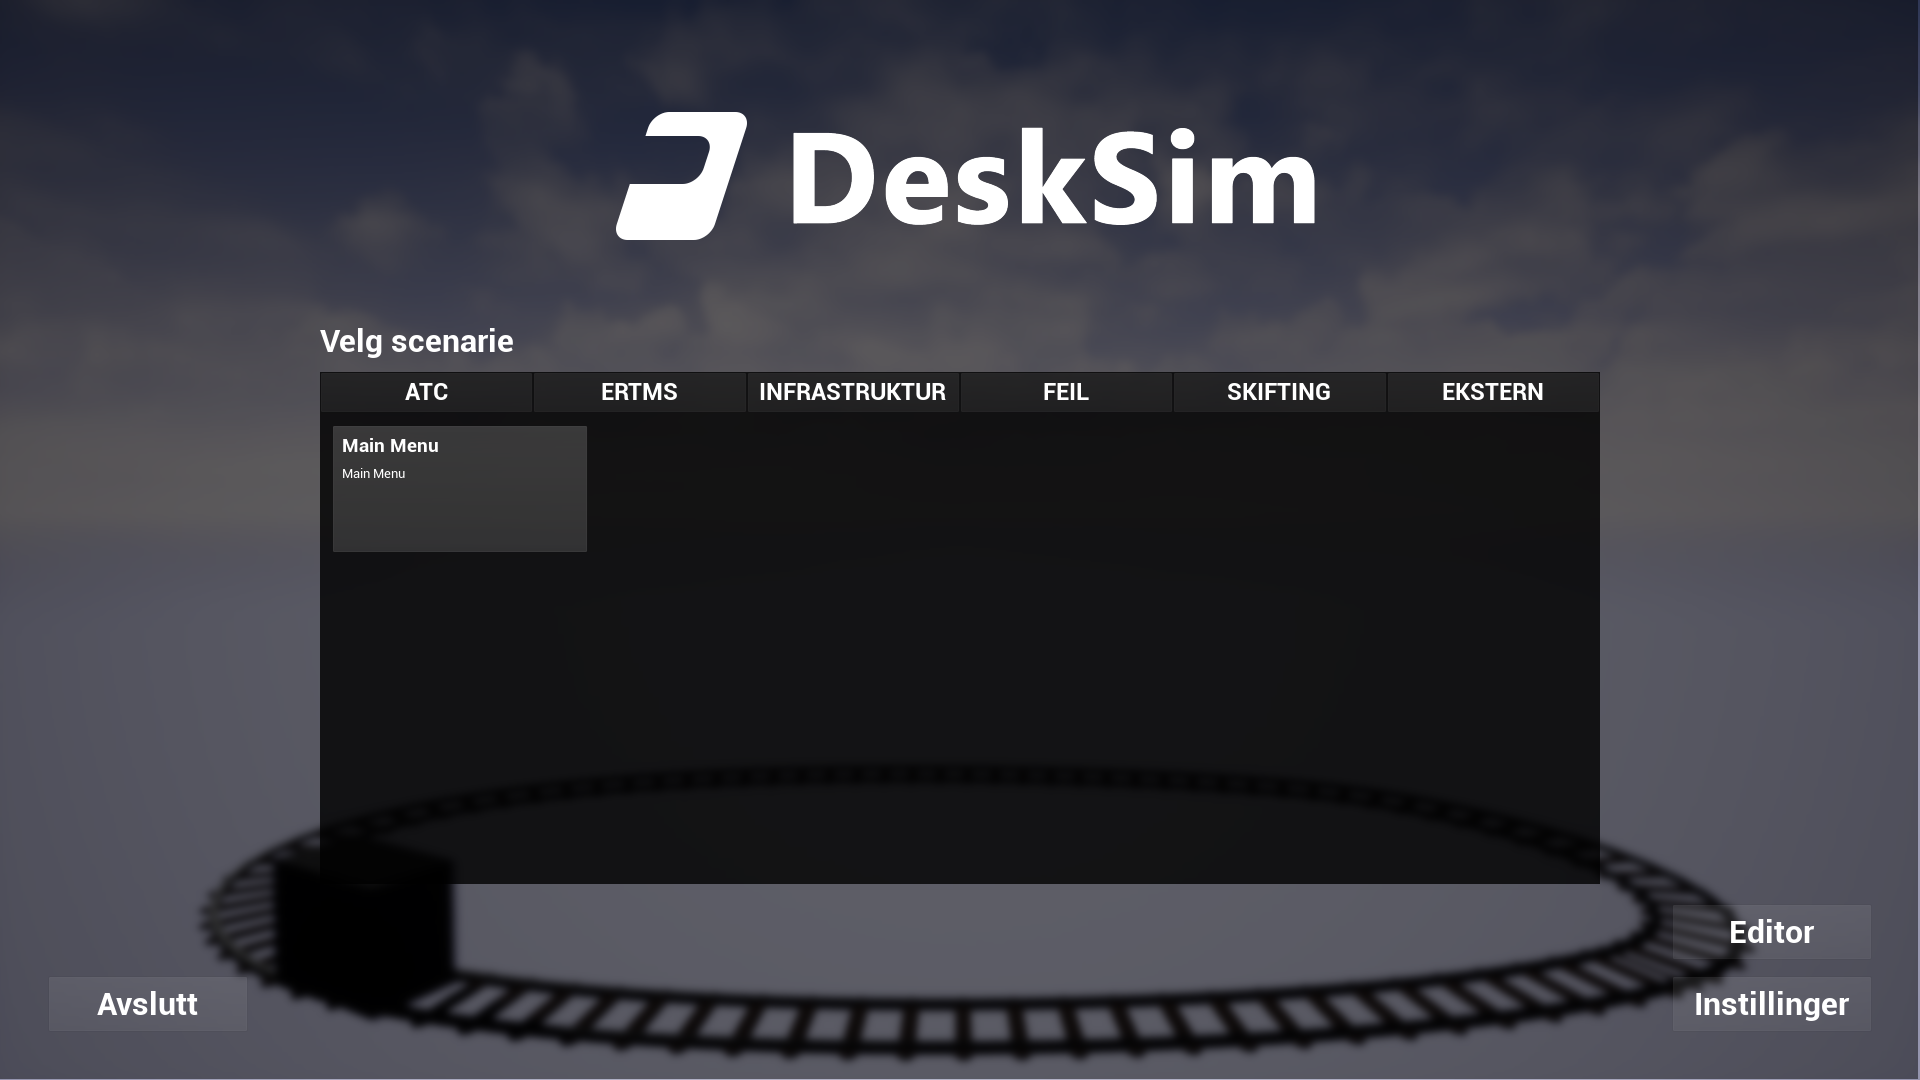
\includegraphics[width=0.8\textwidth]{figures/Main Menu.PNG}
    \vspace{12pt}
    \caption{DeskSimV2: Main Menu}
    \label{Main_Menu_img}
\end{figure} 

Pressing the "Settings" button opens up a settings menu which allows the user to change the screen resolution and the window mode for the application. This settings menu is also available in the pause menu of the game, so settings can be changed during scenarios. 

\begin{figure}[H]
    \centering
    \vspace{12pt}
    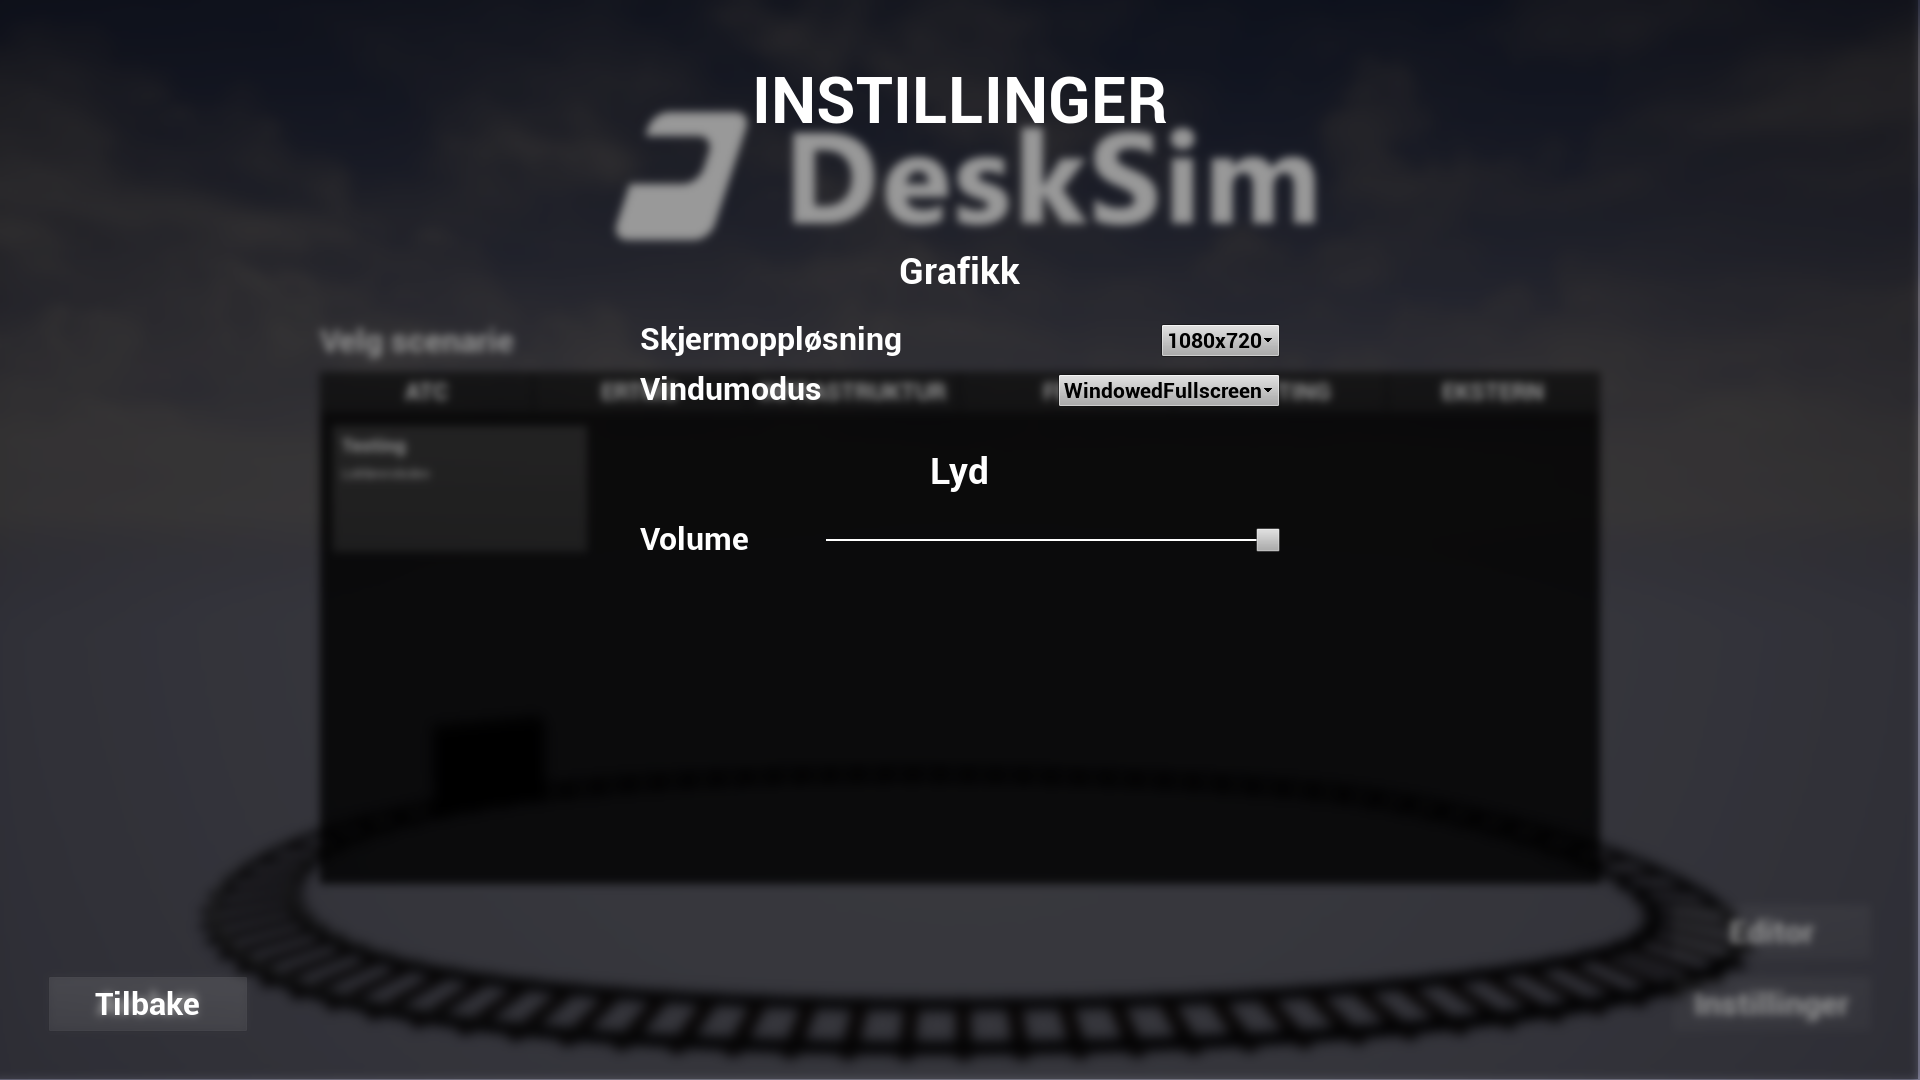
\includegraphics[width=0.8\textwidth]{figures/Settings.PNG}
    %\vspace{-12pt}
    \caption{DeskSimV2: Settings Menu}
    \label{Settings_img}
\end{figure} 

\section{Simulator mode}

The in-game experience consist of a view that corresponds to the view a train driver has from inside the front wagon of a train. The speedometer at the top left of the screen presents the user with the current speed of the train. \todo{legg til mer tekst}
%kamera ser gjennom fronten av toget, hud oppe i venstre viser fart, speedometer, osv. 

\begin{figure}[H]
    \centering
    \vspace{12pt}
    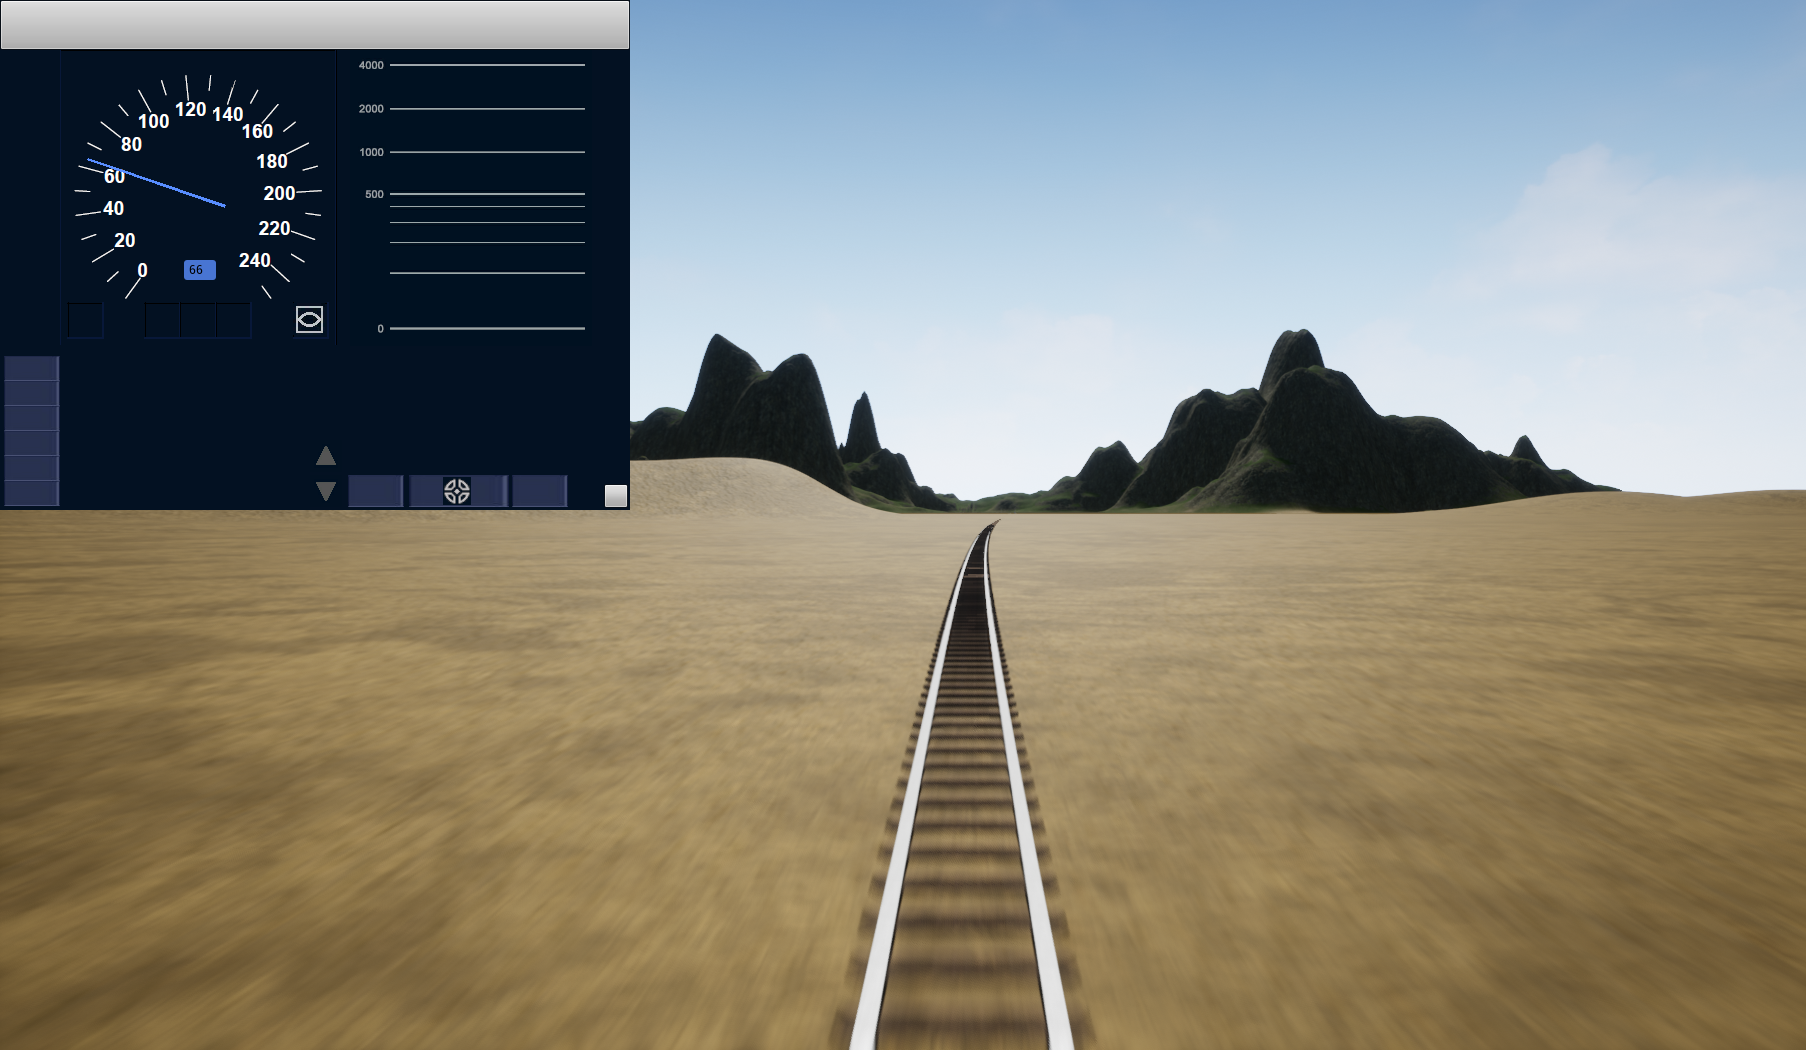
\includegraphics[width=0.8\textwidth]{figures/Tog Drive.PNG}
    %\vspace{-12pt}
    \caption{DeskSimV2: Train Driver View}
    \label{Train_Driver_View_img}
\end{figure}


The user will encounter different signals when running a level/scenario. The signal status and logic are pre-decided and controlled through invisible triggerboxes. These triggerboxes reacts to the position of the train and checks for certain conditions, and can update signal statuses accordingly. 

\begin{figure}[H]
    \centering

    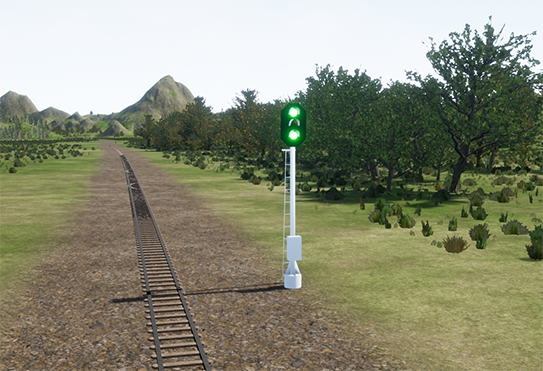
\includegraphics[width=6cm]{figures/Signal1.png}
    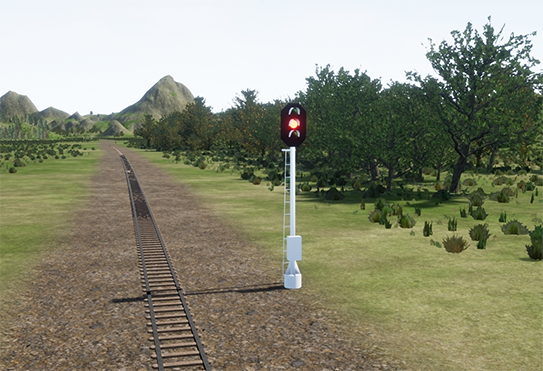
\includegraphics[width=6cm]{figures/Signal2.png}
    %\vspace{-12pt}
    \caption{DeskSimV2: Stop Signal}
    \label{Stop_Signal_img}
\end{figure} 


The simulator provides an option to the user where they can see the world in a drone mode, with free movement and camera rotation. The movement of the drone is independent of the train. 

\begin{figure}[H]
    \centering

    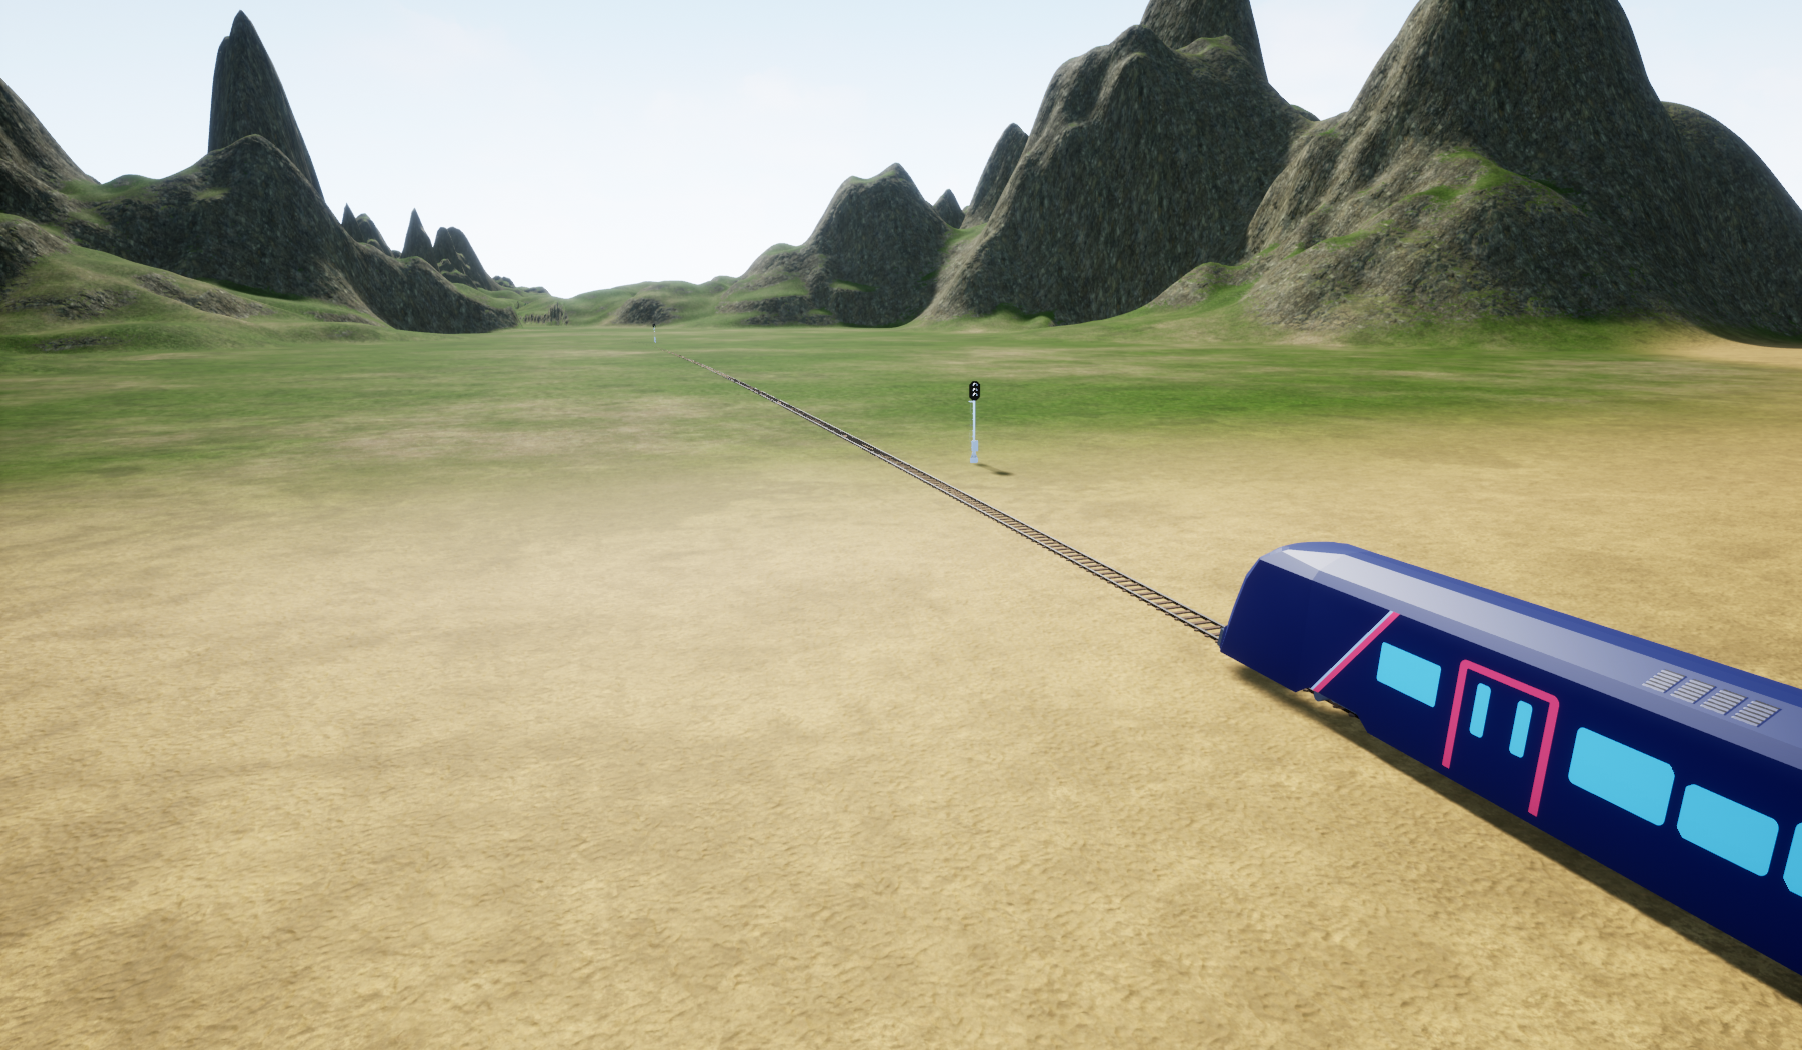
\includegraphics[width=6cm]{figures/DroneMode.PNG}
    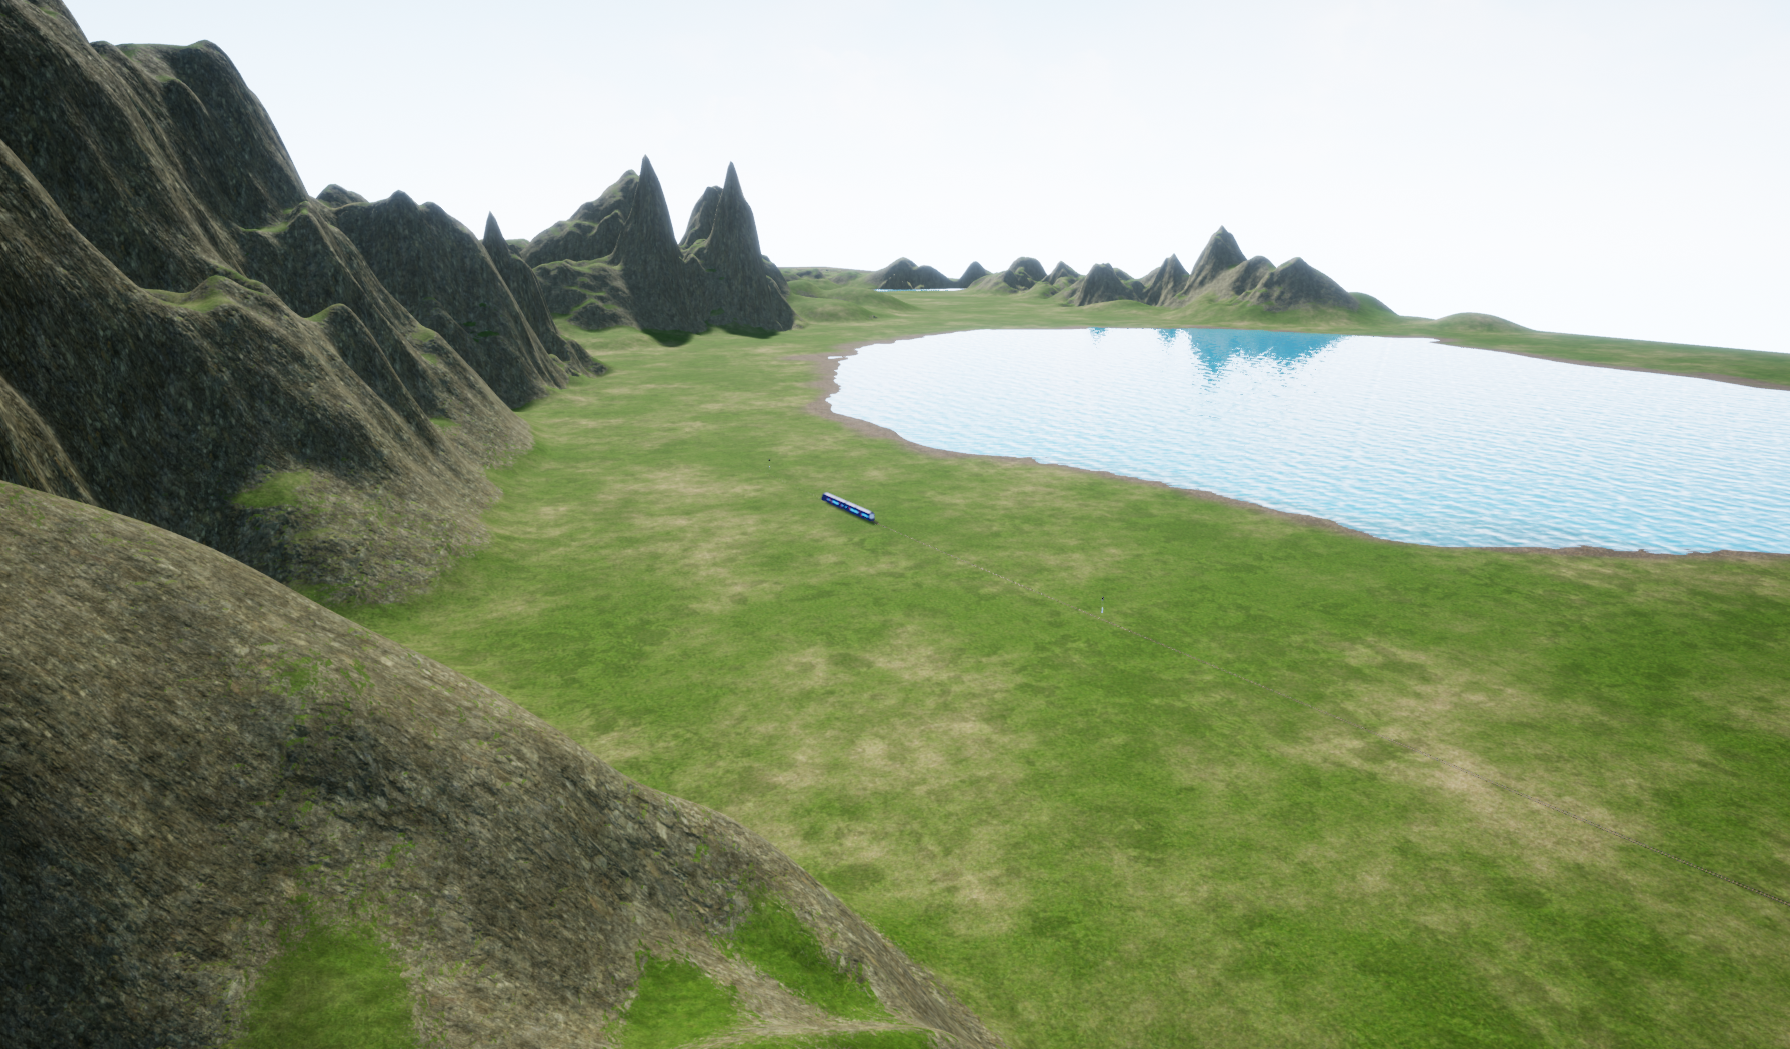
\includegraphics[width=6cm]{figures/DroneMode2.PNG}
    %\vspace{-12pt}
    \caption{DeskSimV2: Drone View}
    \label{Drone_Mode_img}
\end{figure} 

\section{Editor mode}

The editor mode has buttons presented on the top of the screen, where you can save your changes, change the current tool mode and delete objects. The editor mode interface also offers a window for adding new objects to the level. This is done by dragging the icon of the object and dropping it into the level.

\begin{figure}[H]
    \centering

    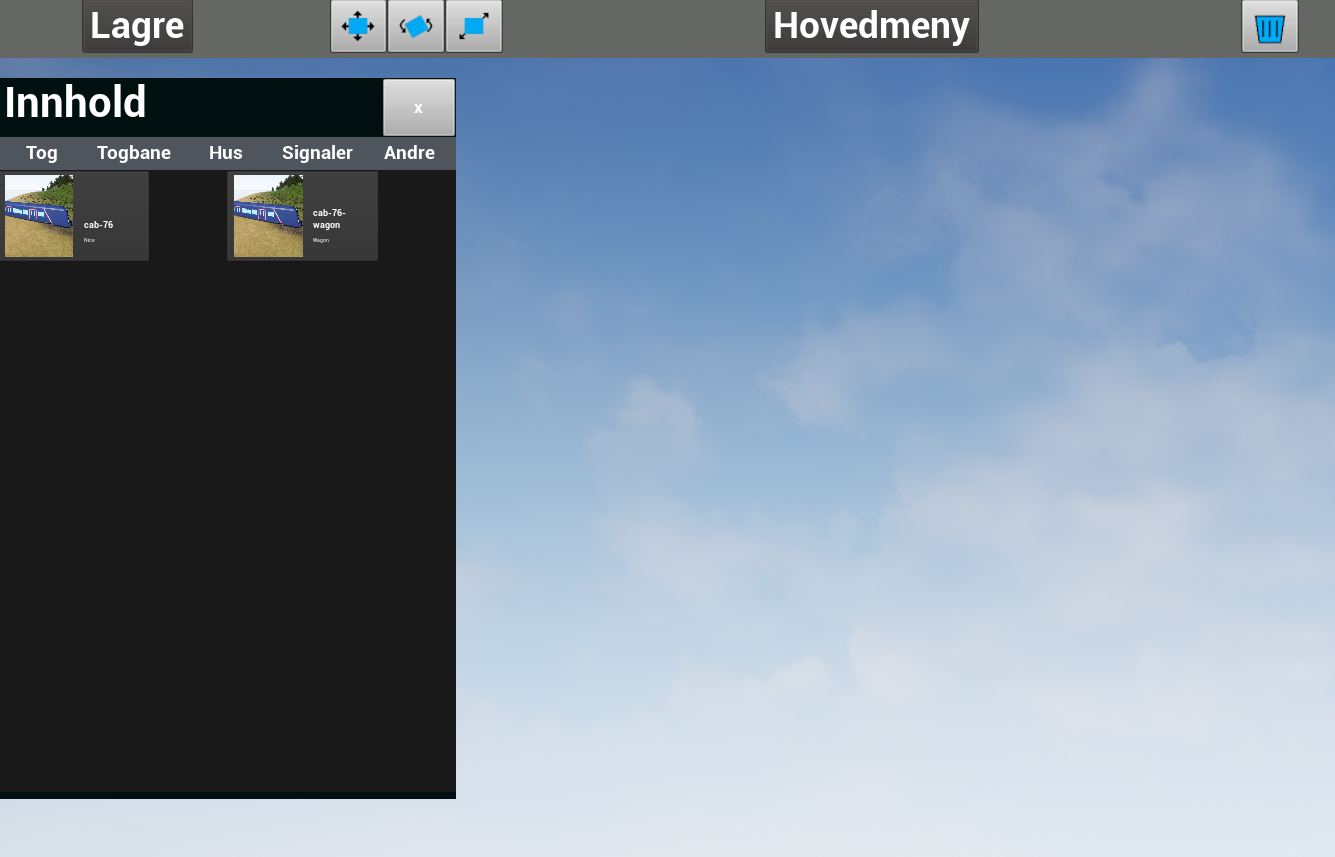
\includegraphics[width=0.9\textwidth]{figures/HUD1.png}
    %\vspace{-12pt}
    \caption{DeskSimV2: Editor Mode HUD}
    \label{Editor_Mode_img}
\end{figure}  \newpage
\chapter{Implementation} \label{implementation_chapter}
\todo{Legg inn kilde for Left Handed, Z Up coordinate system}
This chapter will look closer into the ideas, code and structure behind various parts of the application. all shown code is written by the project group members. One important aspect of Unreal Engine to remember is that the order of axes might be different than other industry standards, as Unreal Engine uses a Left Handed, Z Up coordinate system. (source) In this three-dimensional space, the \textbf{X}-axis points forwards, the \textbf{Y}-axis points to the right, and the \textbf{Z}-axis points upwards.

\todo{Skriv om blueprints, og pipelinen om prototyping i blueprint til cpp}

\section{Game flow} \label{game_flow}

The flow of the game is mostly handled within \verb|EditorHUD.cpp|. The way Unreal handles level switching is by opening levels based on case sensitive \textit{FName} variables. Level changes happens when a user wants to start a scenario from the main menu, and change back to main menu. To decide if the application should open in editor or simulator mode there is a button in the main menu that allows you to change the mode of the main menu. The implementation of this is fairly easy and is displayed below. All scenarios has a menu mode variable that gets updated when the button gets pressed. This, together with a change in the application layout, is the logic behind the applications ability to both play and edit a level.

\begin{lstlisting}[
    caption={Changing menu mode},
    label={lst:cppdoc},
    language=C++]
void AEditorHUD::ChangeMenuMode()
{
	bMenuMode = !bMenuMode;

	// Changing the options for the Menu scenario
	for (int i = 0; i < ScenarioWidgets.Num(); i++)
	{
		ScenarioWidgets[i]->SetMenuMode(bMenuMode);
	}
	// Changes layout for the menu
	MainMenuWidget->ChangeLayout(bMenuMode);
}
\end{lstlisting}

When a game is opened, the game mode used is either decided by the default blueprint chosen for the level in the editor or it could be set to a gamemode in the options string. Unreal Engine does not yet have a visually appealing approach for handling gamemode changes during runtime, and this statement is supported by the community \cite{ue4_change_gamemode}. The negative aspect of this is that creating the functionality for this may in some cases look a bit messy as shown in the code listing \ref{lst:gamemode} .

\begin{lstlisting}[
    caption={Changing game mode at runtime. The code is not the full implementation, but a modified version to show the changing of game modes at runtime.},
    label=lst:gamemode,
    language=C++]
    FString GameMode;
	GameMode = "?Game=/Game/Blueprints/UI/CDerivedEditor/BP_EditorGameMode.BP_EditorGameMode_C";

	UGameplayStatics::OpenLevel(GetWorld(), MapNameReference, true, GameMode);
}
\end{lstlisting}

Another important aspect of the game flow is how the levels is accessible for the users and for further development. When a new level has been created by a developer, a developer can easily add the level to the main menu through a structure located in the \textit{EditorHUD} blueprint. This implementation works because the blueprint is derived from the \verb|EditorHUD.cpp| file and using the macros \textit{UENUM}, \textit{USTRUCT} or \textit{UPROPERTY} as shown in code listing \ref{lst:uproperty} exposes the variable to the editor and adds it to Unreal Engines memory system \cite{uproperty_macro_explanation}. 

\begin{figure}[H]
\centering
  \begin{minipage}{.48\textwidth}
  \begin{lstlisting}[
    caption={UPROPERTY macro.},
    label={lst:uproperty},
    language=C++]
    USTRUCT(BlueprintType)
struct FMMObjectStruct
{
    GENERATED_BODY();

    UPROPERTY(...)
    ECategoryMM Category = ECategoryMM::ATC;
    UPROPERTY(...)	
    FString Name;
	UPROPERTY(...)
	FString Description;
	UPROPERTY(...)
	FName MapName;
};
UPROPERTY(...)
TArray<FMMObjectStruct> MMObjects; ///< All objects
}
\end{lstlisting}
  \label{fig:test2}
\end{minipage}
\begin{minipage}{.48\textwidth}
  \centering
    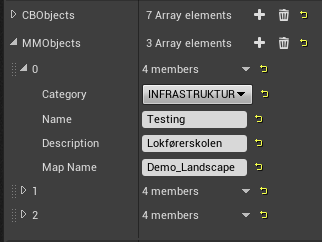
\includegraphics[width=0.90\linewidth]{figures/EditorHUD_MMObjects.PNG}
  \captionof{figure}{The module hierarchy for simulating mode}
  \label{editorMMobj}
  \end{minipage}
\end{figure}

\section{Spline Tool}

One of the first goals specified by the client was to move the train along a straight path. Seeing as a later goal was to also implement curvature, we decided that it would be beneficial to begin work on curved train movement right away, as this would likely save us some time. In the existing simulator, the railway is procedurally generated from a list of points forming a \textit{spline}. A spline can be defined as a mathematical function to interpolate and form a smooth curve between multiple points. Each point is made up of a location vector and a tangent vector for specifying the curvature of the spline at the given position. We also looked into \textit{Bézier curves}, a similar alternative to splines, but Unreal Engine's built-in spline component made it an obvious choice. \newline

\begin{figure}[h]
    \centerline{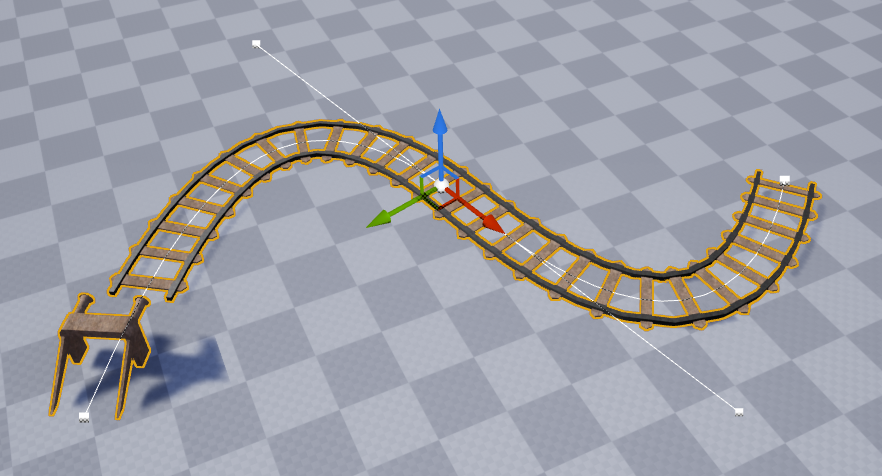
\includegraphics[width=0.9\textwidth]{figures/Spline1.png}}
    \caption{A selected spline deforming a railway mesh along itself. The white squares indicate the spline points, and the white lines indicate the tangent of the selected spline point.}
    \label{SplineFigure}
\end{figure} 


We created \verb|SplineActor.cpp|, a class for handling all functionality related to the railway. This class contains a \textit{USplineComponent}, a powerful component with functions for placing and deforming a mesh along a spline. In this context, a mesh can be described as a 3D-model. The way this initially works is by looping over all points in the spline, placing a sub-mesh that is stretched between points $P_n$ and $P_{n+1}$, and bending the meshes by the curvature of the tangents between $T_n$ and $T_{n+1}$. The spline points were defined by the user in the editor, and could be placed freely. The results looked promising, but a major flaw of this method occurs when any distances between each set of spline points aren't uniform. The meshes would stretch differently along the spline, making the railway look rather odd. A good analogy is imagining a skyscraper with a single, horizontally stretched window instead of separate windows on each floor. The solution to this was to split the spline into segments of equal length to that of the mesh/model itself, and add a new sub-mesh at each segment. Essentially cutting up the railway into pieces and replacing the existing spline points. The mesh used in figure \ref{SplineFigure} is a small slice of a railway created with primitive shapes in \textit{Asset Forge}, a third party software.\footnote{Asset Forge, \url{https://assetforge.io/}} \\

% CODE


% SKAL FJERNE MASSE AV KODEN DONT WORRY "IM WORRIED!!! - HENRIK"

\begin{lstlisting}[
    caption={Initialization of spline points},
    label=lst:cppdoc,
    language=C++]

// Get the size vector of the mesh
const FVector MeshSize = Mesh->GetBoundingBox().GetSize();
	
// Get the length of the bounding box of the mesh along the forward axis
const float MeshLength = MeshSize.X;

...

const float SplineLength = SplineComponent->GetSplineLength();

// Set number of spline points to number of meshes fitting inside spline length
const int SplinePoints = FMath::CeilToInt(SplineLength / MeshLength);

for (int PointCount = 0; PointCount < SplinePoints; PointCount++)
{
	// Generate a spline mesh component for each point in the spline
	USplineMeshComponent* SplineMesh = 
	NewObject<USplineMeshComponent>(
	    this, USplineMeshComponent::StaticClass()
	);

	...
	
	// Get the location and tangents for the mesh at the 
	// current distance along the spline
	
	const float StartDistance = MeshLength * PointCount;
	
	FVector StartPoint = GetLocationAtDistanceAlongSpline(
	    StartDistance, ESplineCoordinateSpace::Local
    );
	    
	FVector StartTangent = GetDirectionAtDistanceAlongSpline(
	    StartDistance, ESplineCoordinateSpace::World
    );
    
	// Get the location and tangents for the end of the 
	// mesh at the current distance along the spline

	const float EndDistance = MeshLength * (PointCount + 1);
	
	FVector EndPoint = GetLocationAtDistanceAlongSpline(
	    EndDistance, ESplineCoordinateSpace::Local
	);
	
	FVector EndTangent = GetDirectionAtDistanceAlongSpline(
	    EndDistance, ESplineCoordinateSpace::World
	);
	
	...
	
	// Set the mesh location and curvature in spline
	SplineMesh->SetStartAndEnd(
	    StartPoint, 
	    StartTangent, 
	    EndPoint, 
	    EndTangent
    );
}
\end{lstlisting}


Opting for a custom spline class instead of Unreal Engine's own solution let us create a railway from a spline. We added specific elements such as \textit{buffer stops}, the metal bars at the end of a railway to stop trains, as seen in figure \ref{SplineFigure}. We added an optional parameter to the \verb|SplineActor.cpp|, where the user can input a separate mesh to be displayed as the first and/or the last sub-mesh of the spline. However, if this field is left empty, the sub-mesh will default to the given railway mesh. We also implemented a boolean flag which sets off if the spline extends a desired angle or curvature limit, to ensure the train looking natural when traversing the railway. \newline

\begin{figure}[h]
    \centerline{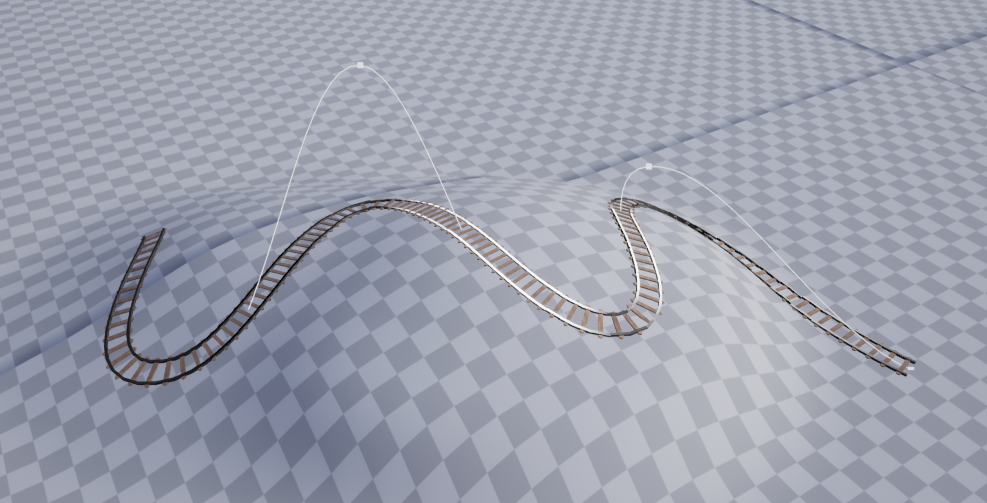
\includegraphics[width=0.9\textwidth]{figures/Spline2.png}}
    \caption{A railway conforming to the terrain height}
\end{figure} 

One of the challenges with the tool occurred when manually placing the spline points. The railway curved naturally in the horizontal plane, but if the terrain had any difference in height, the railway would simply disappear under ground or hover above ground. To solve this, we perform a line cast in each spline point's X- and Y-coordinates, from the top to the bottom of the level. This is a way to see if we hit any terrain along the line cast. If there is a hit, the Z-coordinate of the relevant spline point is simply set to the height value of the terrain hit. This gets more computationally expensive the longer a spline is, but is only run once when a spline undergoes change, so any noticeable effects are minuscule. 
% kjør oppdatering av spline i en annen thread? da slipper editoren å lagge så mye når man endrer på ting. fant en plugin som bruker spline greier i en annen thread, men koster penger. Skal gå ann å lage en ny thread, gjøre computations der og sende det tilbake i game thread. - EH


\section{Signal controller}

The \textit{CentralSignalController} class is responsible for signal and status communication between the signals and trains. The controller receives signal and status updates from either \textit{TrainSignalTriggerBox} or \textit{TrainStatusTriggerBox}, which are placed along the railway and are used to send signal or status updates depending on configured conditions. 

When the level is loaded and the game begins, the \textit{CentralSignalController} searches for all actors inheriting from the \textit{BasicSignal} class. Valid actors are then sorted into lists based on which type they are, such as \textit{MainSignal} or \textit{ForwardSignal}. These different lists are then used later to send signal updates. 

\begin{lstlisting}[
    caption={Finds and stores all signals based on class},
    label={lst:signal_find_signals},
    language=C++]
void ACentralSignalController::FindAllSignals()
{
	// Finds all actors of signal classes
	UGameplayStatics::GetAllActorsOfClass(GetWorld(), DwarfSignalBP, DwarfSignalActors);
	UGameplayStatics::GetAllActorsOfClass(GetWorld(), MainSignalBP, MainSignalActors);
	UGameplayStatics::GetAllActorsOfClass(GetWorld(), ForwardSignalBP, ForwardSignalActors);

	int32 i = 1;

	// Loops through all actors
	for (AActor* DwarfSignalActor : DwarfSignalActors)
	{
		ABasicSignal* DwarfSignal = Cast<ABasicSignal>(DwarfSignalActor);
		if (DwarfSignal)
		{
			FString TagName = FString::Printf(TEXT("Dwarf_%i"), i++);
			
			DwarfSignal->Tags.Add(FName(TagName));

			AllSignalActors.Add(DwarfSignalActor);
		}
	}
	...
}
\end{lstlisting}

When the controller receives a signal update, an ID, new signal state and signal type must be specified. The controller then searches through the specified signal list to match the IDs, and when this happens the new signal state is sent. The controller continues searching the list, if more than one signal shares the same ID. Given that the length of the list of signals is quite short, the time spent searching the list even when the first match is found is insignificant. % measure this? or at least prove the time spent will have a small to none effect on fps

\begin{lstlisting}[
    caption={Updates signals based on ID and type},
    label={lst:signal_updates},
    language=C++]
void ACentralSignalController::SendUpdatedSignal(FName SignalID, ESignalType SignalType, ESignalStatus Status)
{
	TArray<AActor*> Actors;

	// Selects relevant actors to search based on signal type
	switch (SignalType)
	{
	case ESignalType::Main:
		Actors = MainSignalActors;
		break;
	case ESignalType::Forward:
		Actors = ForwardSignalActors;
		break;
	case ESignalType::Dwarf:
		Actors = DwarfSignalActors;
		break;
	default:
		checkNoEntry();
		break;
	}

	// Loops through all signals
	for (AActor* SignalActor : Actors)
	{
		ABasicSignal* Signal = Cast<ABasicSignal>(SignalActor);
		if (Signal && (Signal->ID == SignalID))
		{
			// If the signal matches the incoming id, update the status
			Signal->UpdateSignalStatus(Status);
		}
	}
}
\end{lstlisting}

As the Central Signal Controller is an actor, it needs to be placed in every level which is going to use signals. One alternative would be to create a subsystem with the same functionality. This would allow the controller to work in any level without needing to place an actor, as well as having a more predictable and stable lifecycle. 

\section{Signals}

The class \textit{ABasicSignal} is used for the three different types of signals. The three signal types share the same functionality, with the only difference being the models used and number of lights on each model, as well as which colors are used and how the signal reacts to signal status updates. 

Each signal type is stored as a blueprint which stores the model used, as well as signal-type specific information such as what colors are used and how the signal reacts to signal status updates. This way only one \cpp code file is used for all signals, which makes it easier to implement new features or fix bugs, in addition to improving maintainability. 

\begin{figure}[h]
    \centerline{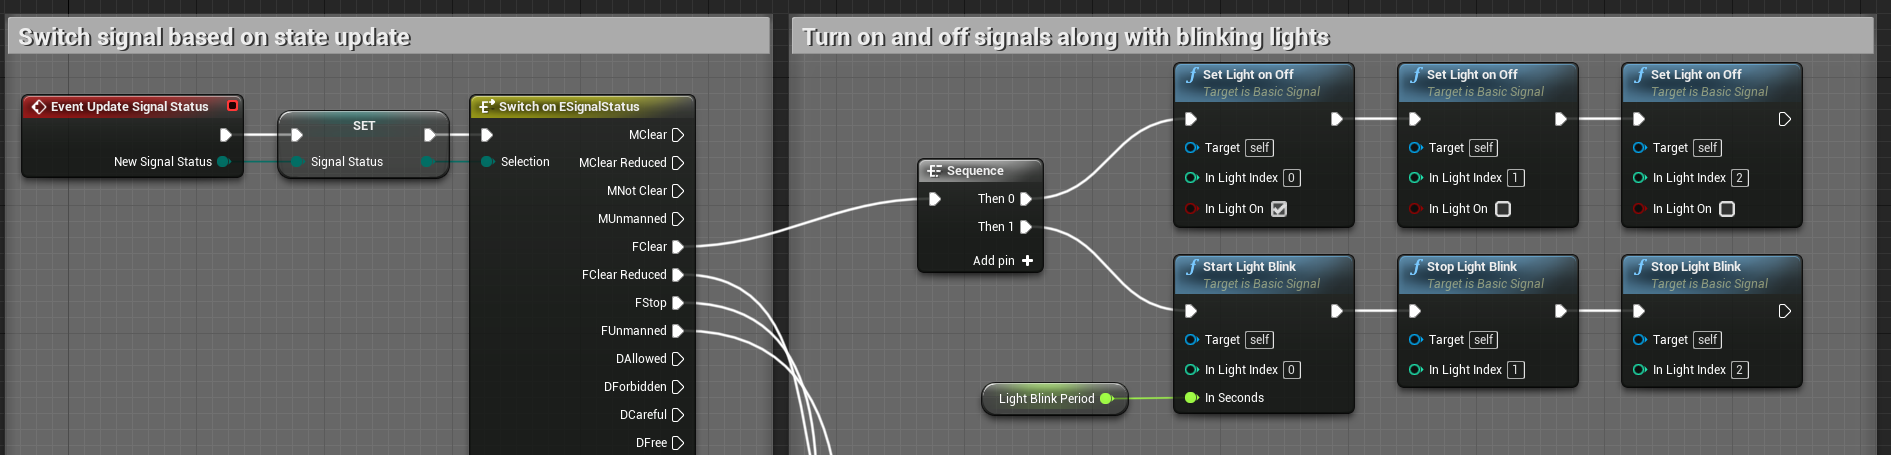
\includegraphics[width=1\textwidth]{figures/Signal_switch.png}}
    \caption{Blueprint showing how a signal switches status}
\end{figure} 

Because the different signals use different models, hard-coding the positions of the signal lights is not an option. Instead sockets are placed on the models in the Unreal Editor, which are used to dynamically place signal lights at runtime. When the game starts playing spheres are created and placed according to the sockets on the model. A standard naming convention is used for sockets and components. The socket names need to match the socket names on the static mesh model, in order for the positioning to be correct. 

When components are created during runtime it is important to manually register the component, otherwise it will immediately be garbage collected and disappear. \todo{this was an interesting bug/issue to learn about, write more about it?}

\begin{lstlisting}[
    caption={Creates dynamic instanced materials for each signal light},
    label={lst:signal_lights},
    language=C++]
void ABasicSignal::SetupLight()
{
	RemoveLights();

	// Create all lights in a loop
	for (int32 i = 0; i < NumLights; i++)
	{
		FString SocketName = FString::Printf(TEXT("Socket_%i"), i + 1);
		FString LightMeshName = FString::Printf(TEXT("LightMesh_%i"), i + 1);

		UStaticMeshComponent* LightMesh = NewObject<UStaticMeshComponent>(this, FName(LightMeshName));

		// Creates a new light struct
		FSignalLight NewLight(LightMesh);

		NewLight.LightMesh->SetStaticMesh(BaseLightMesh);

		NewLight.LightMesh->SetupAttachment(VisualComponent, FName(SocketName));

		// Creates the instanced dynamic light material
		NewLight.DynMaterial = UMaterialInstanceDynamic::Create(BaseLightMaterial, this);

		NewLight.DynMaterial->SetScalarParameterValue("Emissive_Strength", MaxLightLevel);
		NewLight.DynMaterial->SetVectorParameterValue("Emissive_Color", FLinearColor(1.0f, 1.0f, 1.0f));

		NewLight.LightMesh->SetMaterial(0, NewLight.DynMaterial);

		NewLight.LightMesh->RegisterComponent();


		Lights.Add(NewLight);
	}
}
\end{lstlisting}

A new \Gls{instanced dynamic material} is created for each sphere, which uses emissive lighting for the signal lights. The new dynamic instance of the material allows material parameters to be changed during runtime for each different instance, ensuring the lights can change independent of other light signals of the same type. 

\begin{figure}[h]
    \centerline{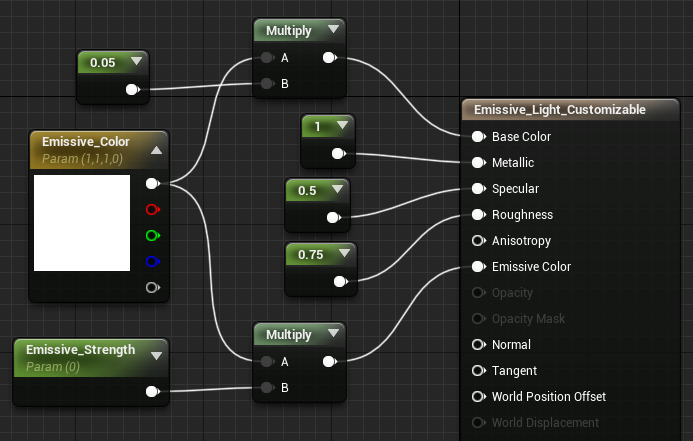
\includegraphics[width=0.9\textwidth]{figures/Emissive_Light_Material.png}}
    \caption{The material used for signal lights}
\end{figure}

The material used for the signal lights is created from scratch in Unreal, using its Material Editor tool. The material has two public parameters which are used to change the color of the material as well as the brightness of the \Gls{emissive light}. The material uses the same color for both the base color and emissive color. The base color has a constant low brightness, which is used for the off state. The emissive color strength is determined by a parameter. All values used range from 0 to 1, with the exception of emissive light strength which can be any value above 0. Higher values results in brighter emissive lights. Currently the entire model using the material lights up as an emissive light source, but a texture could be used to only use parts of the model as an emissive light source.


\section{Login and authentication}

The \textit{ULoginWidget} class contains the functionality used to log in, which uses the \textit{VaRest} plugin to encode, decode, send, and receive web requests. The user data is stored in a struct in \textit{UDesksimGameInstance}, which is a class that is instantiated at the beginning of the application and lives until it is closed, ensuring the user data is available for the entire duration of the application. 

Our application connects with the existing login solution in use at Lokførerskolen. Two endpoints are used, where the first takes a username and password and returns a \acrfull{jwt} on success. The second endpoint takes this \acrfull{jwt} and returns a user object containing various data. This data is then decoded and stored in the gameinstance class, \textit{UDesksimGameInstance}. The application does not verify the \acrfull{jwt} in any way, it just passes it on to the next endpoint. While the \acrfull{jwt} is valid for a long duration, it is not stored in any files, and a new token is requested each time the user logs in. 

% vis kode som decoder og lagrer login info
\begin{lstlisting}[
    caption={Decodes and stores info from userinfo JSON response},
    label={lst:auth_userinfo},
    language=C++]
void ULoginWidget::ReadUserData(UVaRestJsonObject* JsonObj)
{
	UDesksimGameInstance* GameInstance = Cast<UDesksimGameInstance>(GetGameInstance());

	GameInstance->bIsLoggedIn = true;

	// Set Userinfo in gameinstance
	GameInstance->UserInfo.bIsAuthenticated = true;
	
	GameInstance->UserInfo.bIsEnabled = JsonObj->GetBoolField(TEXT("isEnabled"));
	
	GameInstance->UserInfo.id = JsonObj->GetIntegerField(TEXT("id"));
	
	GameInstance->UserInfo.Username = FName(*JsonObj->GetStringField(TEXT("username")));
	
	GameInstance->UserInfo.SubscriptionID = JsonObj->GetIntegerField(TEXT("subscriptionId"));


	// Find info about subscription and user groups
	UVaRestJsonObject* Subscription = JsonObj->GetObjectField(TEXT("subscription"));
	
	TArray<FString> GroupNames = Subscription->GetStringArrayField(TEXT("userGroupNames"));

	// Checks which type the user is
	if (GroupNames.Contains("Administrator"))
	{
		GameInstance->UserInfo.UserType = EUserType::Admin;
	}
	else if (GroupNames.Contains("Ansatte"))
	{
		GameInstance->UserInfo.UserType = EUserType::Teacher;
	}
	else //if (GroupNames.Contains("Student"))
	{
		GameInstance->UserInfo.UserType = EUserType::Student;
	}
}
\end{lstlisting}

The login functionality uses the VaRest plugin to handle common tasks like encoding and decoding \acrshort{json} objects. The plugin was chosen to simplify the use of REST communication.

\section{Editor Mode}
The goal of the editor mode was to give the client a simple tool build worlds and train scenarios. Our task was to implement the ability to place, move and rotate objects such as trains and buildings, and a way to lay a railway across the terrain. We decided to design this tool based on the tools available in Unreal Engine's own editor, as these would accomplish similar tasks. For moving objects around, we created a \gls{gizmo} consisting of one arrow for each axis, and a square for the plane along the X- and Y-axes. Once an object is selected, this gizmo appears at its position, utilizing custom depth rendering, which enables the gizmo to always be visible even when it is covered by another mesh. 

\begin{figure}[h]
\centering
\begin{minipage}{.5\textwidth}
  \centering
  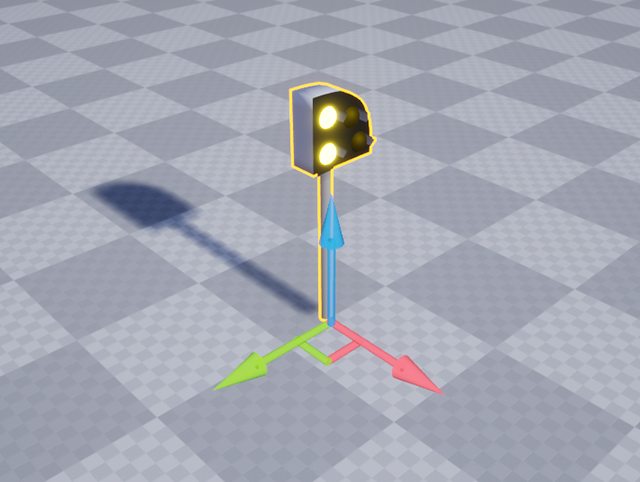
\includegraphics[width=0.95\linewidth]{figures/Gizmo1.png}
  \captionof{figure}{The translation gizmo on a selected signal}
  \label{fig:test1}
\end{minipage}%
\begin{minipage}{.5\textwidth}
  \centering
  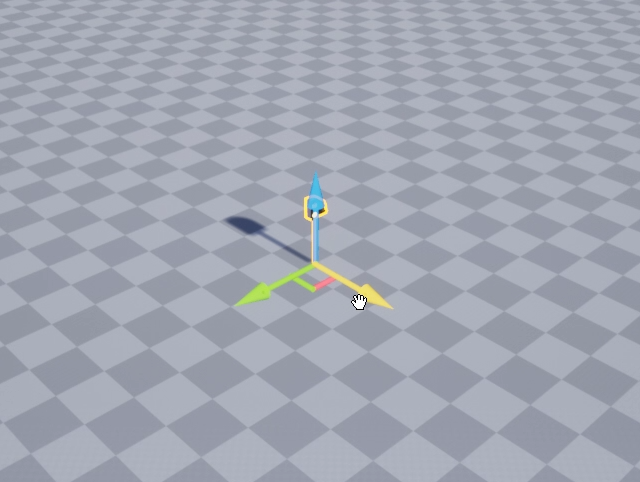
\includegraphics[width=0.95\linewidth]{figures/Gizmo2.png}
  \captionof{figure}{The translation gizmo far away, hovering the X-axis arrow}
  \label{fig:test2}
\end{minipage}
\end{figure}

By hovering the mouse over one of the gizmo's arrows and dragging, the user can move the object in the relevant axis. This is done by casting a line from the camera, in the direction of the cursor's position on the screen, and processing the results on hit. This is done in a separate collision layer for gizmos, such that the line is not obscured by any object. The tool includes two modes, translation and rotation. When switching mode to rotation, the arrow meshes are replaced by a cogwheel in the XY-plane, which rotates the object around the Z axis when dragged. These gizmos are made to be a part of the user interface, and get scaled based on their distance from the camera to keep their size uniform. 

When grabbing a gizmo arrow to move an object, the position of the cursor is saved as a variable in the first frame of holding down the mouse button. This position is used to get the offset between the gizmos center position (also the object anchor position), and the cursor. While dragging the gizmo arrow, the objects position is set to the location of the cursor minus the offset, resulting in the object moving in parallel with the cursor. This behaviour works fine in theory, but during testing, we found a lack of user friendliness due to the cursor being required to overlap the gizmo during dragging. To combat this, we added secondary meshes to each arrow that would inflate the area of interaction. These meshes were given an invisible material, so the user could not see them, but were able to interact with them.

\begin{figure}[h]
\centering
\begin{minipage}{.5\textwidth}
  \centering
  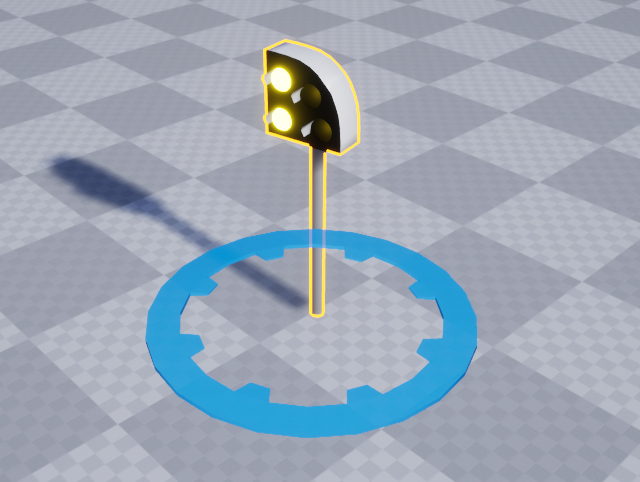
\includegraphics[width=0.95\linewidth]{figures/Gizmo3.png}
  \captionof{figure}{The rotation gizmo in the XY-plane}
  \label{fig:test1}
\end{minipage}%
\begin{minipage}{.5\textwidth}
  \centering
  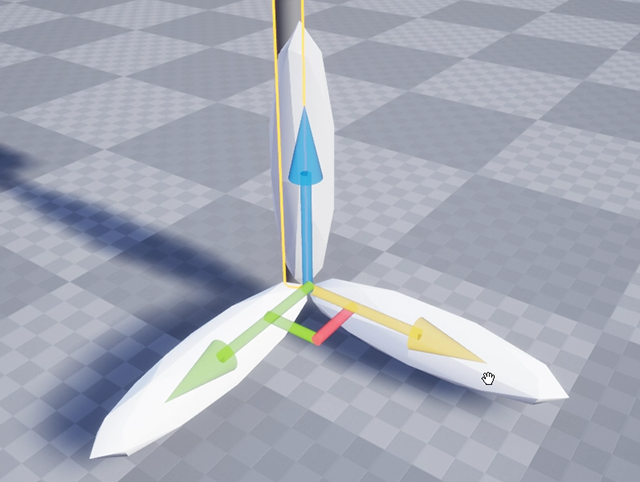
\includegraphics[width=0.95\linewidth]{figures/Gizmo4.png}
  \captionof{figure}{Additional meshes around the arrows}
  \label{fig:test2}
\end{minipage}
\end{figure}

\todo{Forklar litt rundt figurene i teksten}

During user testing with the client, it was made clear that this interaction was still hard, as the cursor would, more often that not, exit the area of these meshes. This was towards the very end of the development, and there was not enough time to iterate on this implementation, as it would quickly grow complicated. But due to the curious nature of programmers, we were attracted towards finding a solution to this problem, even if we did not have the time to finish the implementation of these ideas. We came up with several possible solutions that could fix or recreate this system entirely.


One such idea was to spawn large collision planes at the objects position, when the mouse is dragging an arrow. If the user is moving the object, the plane should stretch like a wall along the relevant axis. It should not be visible to the player, but act as a giant safety net, such as the ones seen at golf courts, to capture the depth of the mouse cursor in the relevant axis. This would provide a more intuitive movement system, where the user could drag the object to it's desired position without keeping the cursor over the gizmo at all times. Another idea for a solution would be to take the cursor's two-dimensional position on the screen and rotate the vector based on the angle between the camera and the object. This may also result in clunky movement, as 2D does not always translate well to 3D when forced.

\section{Landscape and texturing}
% Landscape texture - John Ole 


There was originally a planned runtime terrain editing tool for the simulator, but it became obvious that such functionality would take a considerable amount of time and was therefore taken out of the project scope. This will be further discussed in [discussion::editor] 
\todo{Link discussion}

\section{Save Functionality}
The meaning of saving the game can vary from game to game, but the idea behind it is to save information about something persistent. Say you quit and re-open the game, you should be able to resume where you left off. In this project we have implemented an editor mode where the player can edit and change the world/level they are playing. But for the editor mode to serve its purpose we need to be able to save the changes we made to the level so we can open it in play mode after and view the changes. 

Our \textit{SaveLevel} class inherits from Unreal`s \textit{SaveGame} class which is used to preserve information across multiple play sessions. We mainly save the transform of placed or edited objects in the scene, but also general data and identifiable data such as name, class and level name. All the information from the actors saved is stored inside a array in a \verb|.sav| file which is the save file format Unreal Engine 4 uses.

\todo{code caption and label}

\begin{lstlisting}[
    caption={SaveLevel class that holds all data that is saved},
    label={lst:SKRIVHER},
    language=C++]
/**
 * @brief Struct holding all Data needed from an Actor.
 */
USTRUCT()
struct FActorData
{
    ...

public:
    /* Identifier for which Actor this belongs to */
    UPROPERTY()
        FName Name;
	
    /* Class of the Actor */
    UPROPERTY()
        UClass* Class = nullptr;;

    /* For movable Actors, keep location,rotation,scale. */
    UPROPERTY()
        FTransform Transform;

    /* Contains all 'SaveGame' marked variables of the Actor */
    UPROPERTY()
        TArray<uint8> ByteData;
};

/**
 * @brief Handles what data is saved in the .sav files.
 */
UCLASS()
class DESKSIMV2_API USaveLevel : public USaveGame
{
	...

public:
    ...

    UPROPERTY()
        TArray<FActorData> SavedActors;

    ...
};
\end{lstlisting}

A big issue we had was how we would handle what actors got saved, since a level can often contain many actors many of which we do not edit or create in editor mode and it would be unnecessary to save those actors. We explored different options one of which was to create a base actor class which every save able actor inherits. Although this would not work since the save able actors are of different classes. Instead we created an interface the actors can inherit if they are save able, giving every class the ability to be saved regardless of what their base class is.

\begin{lstlisting}[
    caption={Interface for classes that are save able},
    label={lst:SKRIVHER},
    language=C++]
UINTERFACE(MinimalAPI)
class UIsSaveableInterface : public UInterface
{
	GENERATED_BODY()
};

/**
 * 
 */
class DESKSIMV2_API IIsSaveableInterface
{
	GENERATED_BODY()

	// Add interface functions to this class. This is the class that will be inherited to implement this interface.
public:
};
\end{lstlisting}

An example of how a class can be made saveable by inheriting the interface in the class declaration along side their parent class.

\begin{lstlisting}[
    caption={Example of a class that inherits IsSaveableInterface},
    label={lst:SKRIVHER},
    language=C++]
UCLASS()
class DESKSIMV2_API ATrain : public APawn, public IIsSaveableInterface
{
	...
\end{lstlisting}

All the save functionality is handled by the \textit{SaveManager} which has two main functions, \textit{SaveGame} and \textit{LoadGame}. \textit{SaveGame} handles all the functionality related to saving the current game state into a \verb|.sav| file. It checks all actors classes in the level and if it inherits from the \textit{IsSaveableInterface} interface its data is saved. 

\begin{lstlisting}[
    caption={SaveGame function from SaveManager},
    label={lst:SKRIVHER},
    language=C++]
void ASaveManager::SaveGame()
{
	// Get LevelName to find what to name the .sav file
	LevelName = GetWorld()->GetMapName();

	// Create and instance of SaveGame
	USaveLevel* SaveGameInstance = Cast<USaveLevel>(UGameplayStatics::CreateSaveGameObject(USaveLevel::StaticClass()));
	check(SaveGameInstance);
	// Loop through ALL Actors in Scene
	for (TActorIterator<AActor> It(GetWorld()); It; ++It)
	{
		// Checks if the Actor inherits from IsSaveableInterface
		if (It->GetClass()->ImplementsInterface(UIsSaveableInterface::StaticClass())) 
		{
			AActor* Actor = *It;

			FActorData ActorData;
			ActorData.Name = Actor->GetFName();
			ActorData.Transform = Actor->GetActorTransform();
			ActorData.Class = Actor->GetClass();

			// Creates a memorywriter and archive for Actor Data
			FMemoryWriter MemWriter(ActorData.ByteData);
			FObjectAndNameAsStringProxyArchive Ar(MemWriter, true);
				
			// Only Saves Variables with UPROPERTY(SaveGame)
			Ar.ArIsSaveGame = true;
				
			// Serializes Actors UPROPERTIES into binary
			Actor->Serialize(Ar);
				

			SaveGameInstance->SavedActors.Add(ActorData);
		}
	}

	// Start async save process.
	UGameplayStatics::SaveGameToSlot(SaveGameInstance, LevelName, UserIndex);

	...
}
\end{lstlisting}

The \textit{LoadGame} function in \textit{SaveManager} reads and loads data of the \verb|.sav|-file with the matching file name to the name of the loaded level. Then it updates the data of the existing actors with the matching data from the save file based on the actors name. If it doesn't find the actor from the savefile in the level it will create a new actor with the data from the save file.


\begin{lstlisting}[
    caption={LoadGame function from SaveManager},
    label={lst:SKRIVHER},
    language=C++]
void ASaveManager::LoadGame()
{
	// Get LevelName to find what .sav file to load
	if (!GetWorld()) return;
	
	LevelName = GetWorld()->GetMapName();

	// Create and instance of SaveGame
	USaveLevel* SaveGameInstance = Cast<USaveLevel>(UGameplayStatics::CreateSaveGameObject(USaveLevel::StaticClass()));
	check(SaveGameInstance);
	

	// Load Data from Save file
	SaveGameInstance = Cast<USaveLevel>(UGameplayStatics::LoadGameFromSlot(LevelName, UserIndex));
	if (SaveGameInstance)
	{
		// Iterate through all actors in save and point to their corresponding actor in scene
		for (FActorData ActorData : SaveGameInstance->SavedActors)
		{
			AActor* Actor = FindActorByName(ActorData.Name);
			if (Actor)
			{
				// Updates Actor found in scene
			    Actor->SetActorTransform(ActorData.Transform);
			}
			else
			{
				FActorSpawnParameters SpawnParams;
				SpawnParams.Name = ActorData.Name;
				SpawnParams.SpawnCollisionHandlingOverride = ESpawnActorCollisionHandlingMethod::AdjustIfPossibleButAlwaysSpawn;
					
				// Creates a new Actor with data from save
				Actor = GetWorld()->SpawnActor(ActorData.Class, &ActorData.Transform, SpawnParams);
					
				// Creates a memoryreader and FArchive
				FMemoryReader MemReader(ActorData.ByteData);
				FObjectAndNameAsStringProxyArchive Ar(MemReader, true);

				// Only Filters the Variables with UPROPERTY(SaveGame)
				Ar.ArIsSaveGame = true;

				// Converts serialized binary into Actors UPROPERTIES
				Actor->Serialize(Ar);
					
				...
			}
		}
		...
	}
	...
}
\end{lstlisting}

\section{User Interface / Heads-Up Display} \label{HUD_implementation}

The heads up displays or HUDs of the application is in the context of the simulator a term used to describe all user interface elements in the simulator to provide feedback to the user in the viewport. 

The HUD consist of seven different user widgets. User widgets are Unreal Engine's components that allows for placement of UI elements in the viewport for 3D games. This section will explain the development of the logic that displays the user widgets.

In the first iteration of the user widgets they were created as \gls{blueprint}, this meant that all of the widgets with it's logic was created as a collection of nodes. According to the Unreal Engine forum, blueprints run between 10-40 percent slower than \cpp \cite{ue4_blueprint_forums_2016}. This was one of the reasons we felt that it was necessary to convert the code from blueprint to \cpp files. Another fact is that blueprint coding, as a practise, does not allow us as students to display our skills in both programming and documentation to the same degree.

\begin{figure}[H]
    \centerline{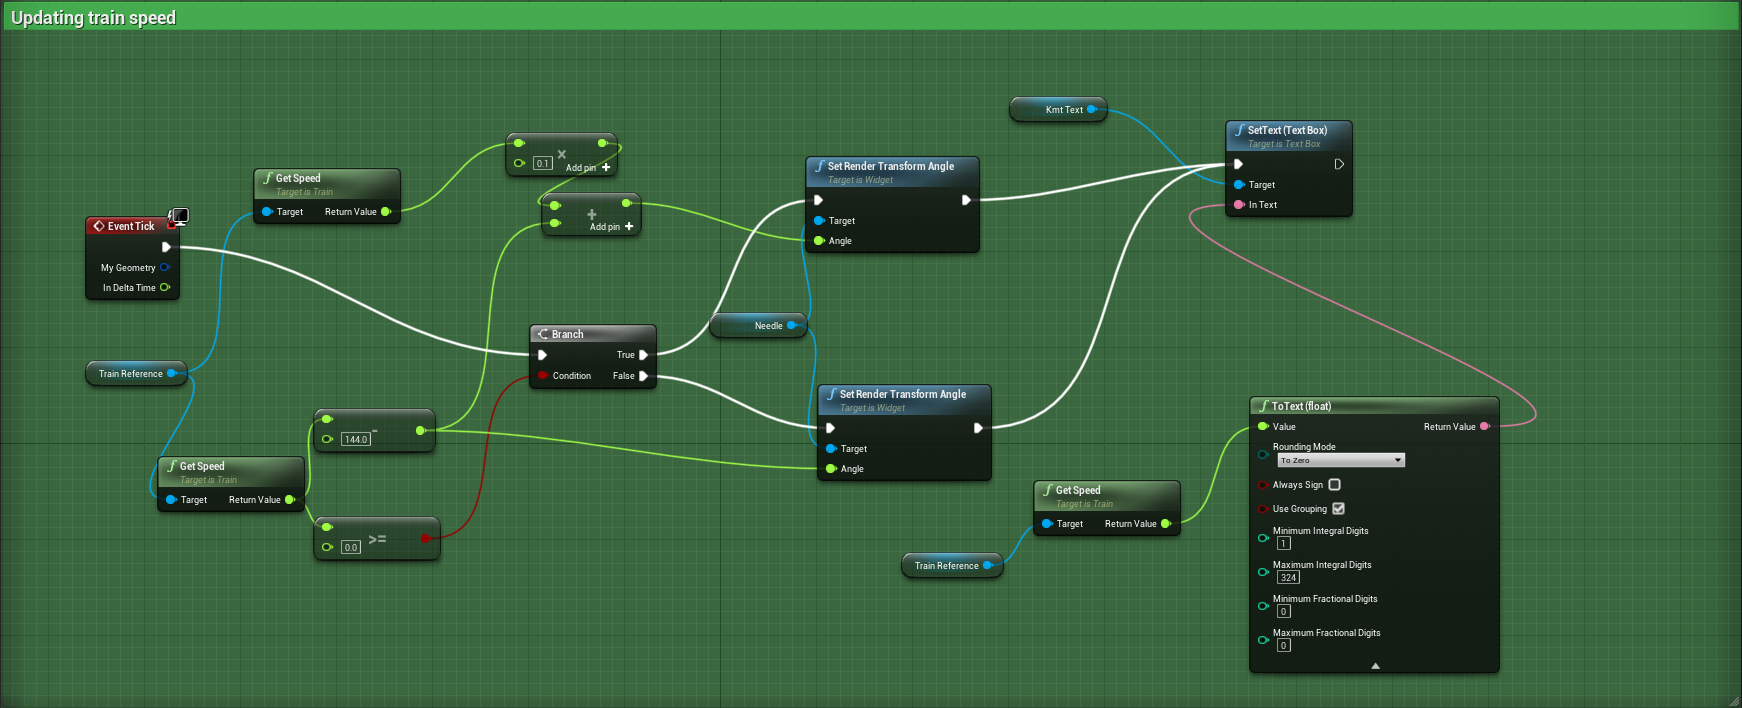
\includegraphics[width=0.9\textwidth]{figures/TrainDMISpeedFunc.PNG}}
    \caption{Update Speed function for the train DMI in blueprint}
    \label{fig:train_dmi}
\end{figure}

Figure \ref{fig:train_dmi} and code listing \ref{lst:updateDMI} contain the same functionality for updating the needle and text of the speedometer displayed to the user. All of the widgets initially created as blueprints got converted to \cpp at some point in the project.

\begin{lstlisting}[
    caption={Update speed function in \cpp},
    label={lst:updateDMI},
    language=C++]
void UTrainDMI::Update(float Speed)
{
	if (Speed >= 0.0)
	{
		float RenderAngleDriving = (Speed * 0.1) + (Speed - 144);

		int Text = FMath::FloorToInt(Speed);
		FString SpeedText = FString::SanitizeFloat(Text, 0);

		UpdateDMI(RenderAngleDriving, FText::FromString(SpeedText));
	}
	else
	{

		int Text = FMath::FloorToInt(Speed);
		FString SpeedText = FString::SanitizeFloat(Text);

		UpdateDMI(Speed - 144, FText::FromString(SpeedText));
	}
}
\end{lstlisting}

The file \verb|EditorHUD.cpp| handles which user widget that is displayed to the user. What the HUD displays is based on what game mode that the game is currently using. The game mode is decided by which part of the application the user is currently in. If the user is in the simulator game mode, the train DMI will be displayed.


\section{Plugins}

The following functionality described in this section is not developed by us but needs to be included as it is used in the simulator.

Unreal Engine did not support the usage of two similar input devices using raw input. We therefore decided to look for the options at hand to solve this issue. The two solutions we found was to purchase and utilize a plug-in created by \textit{Lemontmoon} called \textit{VM Input Manager}\footnotemark[1], or to implement an input mapping system to our own application. We chose to utilize the plug-in and the choice and other options will be described in \todo{Described in discussion}
\footnotetext[1]{\url{https://www.unrealengine.com/marketplace/en-US/product/wm-input-manager}}

The plug-in consists of 18 \cpp classes and 31 blueprints. The benefit this had to our project was that we could just manually map the USB input peripherals during run-time. The plug-in is used only used in the \textit{BP\_GameplayGamemodeBase} blueprint to spawn the necessary widget as a red dot in the top left of the screen. 

The \textit{VaRest} plugin handles common tasks related to performing REST calls. It simplifies the process of working with requests and responses, and provides functions to both simplified and detailed ways to create and send requests. While the plugin is designed to be used in blueprints without any \cpp code, all the functionality is available to be used in \cpp. The same results could be achieved without the use of the \textit{VaRest} plugin, however it would require more work unrelated to the main goal.  \newpage
\chapter{Deployment}

This chapter will detail how the software can be deployed, both for development and release as a packaged product. It will also present how one may compile the code to create and deploy documentation. 

\section{Packaging and release}

Unreal Engine comes with a built-in \gls{packaging} system. The system compiles source code, cooks content and builds the game. The game is then packaged as an executable file and game data is stored in \verb|.pak|-files. The entire folder can be compressed and uploaded to a server where users can download the file, extract the file and play the game without any further installation. This is the simplest solution for deploying the finished product, but requires re-downloading the entire software when updates are packaged and released. A similar system is already in use at \Gls{lokforerskolen}, where the software is downloaded in its entirety and updates requires a complete re-download. Due to its simplicity we will use this solution, however there are more advanced options in \Gls{unrealengine} if a better updating system is required. 

One option to improve the update process is to create an auto-updater and automatically patch the game with new updates. Doing this would most likely require more work than it is worth if the game is not updated often. In Unreal it is possible to use clustering in the \verb|.pak| files, which allows for easier streaming and patching of game data. 

\section{Setting up the project}

The project uses Unreal Engine 4.27. The engine can be installed on the Epic Games Launcher, which is also used as a hub for various features related to Unreal. After the engine is installed, it can be used to open any Unreal Engine 4 project. 

Each Unreal project consists of some standard files and folders, most notably the \verb|.uproject|-file which contains some general info about the project, like engine version, code modules, and plugins used. User-made \cpp code needs to be compiled before the editor can start, which is done by generating a \Gls{visualstudio} \gls{solution} for the project. \Gls{visualstudio} is the default \acrshort{ide} to use with Unreal, but other options are available. After the project is compiled for the first time, additional changes made during development can be compiled in the Unreal Editor, which hot-reloads the changed files. 

Plugins used can be installed in two ways. The first and easiest method is to get the plugin via Unreal Engine's marketplace for assets and install it to an engine. The second method requires some more work, but installs the plugin in the project itself, allowing it to be shared between team members. This is a good way to share paid plugins within a project, Some manual work is required to set this up, mainly involving copying either compiled or source files to the proper directory in the project and adding files to source control to allow sharing. 

There are three main directories shared in an Unreal Project, namely \verb|Source| which contains all the \cpp code written for the project, \verb|Content| which contains all assets like materials, models and blueprints, and \verb|Config| which contains extra configuration files used in various places. A \verb|Plugin| folder is also needed if any plugins are shared in the project. These are the essential folders to track using source control. During startup and use other intermediate folders are created, such as \verb|Build|, \verb|Binaries|, and \verb|Intermediate|. These intermediate folders are automatically generated, and normally should not be included in source control.

\section{Deployment of documentation}

During the development we have used \Gls{doxygen} for documenting code. It lets us compile the source folder into generated HTML files with a formatted documentation of all comments. The resulting webpage is self-contained and features links between related classes and functions. We generated this using \textit{Doxywizard}, which offers a graphical user interface for \Gls{doxygen}. To regenerate this documentation, run Doxygen with \verb|/Source/DeskSimV2| as the source code folder input. The program assumes all code to be commented using the \Gls{doxygen} standard. \footnote{Doxygen Manual, \url{https://www.doxygen.nl/manual/docblocks.html}}
 \newpage
\chapter{Testing}

This chapter explains and elaborates the testing performed on the developed system. 

\section{User Testing}

In collaboration with the client, we set up user tests towards the end of development. We visited \Gls{lokforerskolen} in Oslo and borrowed three students who have previously used their current simulation software. The goal of user testing was to further iterate on the software based on given feedback, but we didn't have a lot of time as the testing was done two weeks prior to the deadline. The tests were done by prompting the user with a set of tasks. These were simple tasks, designed to test the user interface, software structure and overall user experience. The observer measured the time spent, while writing down notes from the user’s performance. The user was also prompted with questions about the experience. We also had a few tests with the client where we tested the editor mode which is only available to admins.

\begin{table}[H]
    \begin{tblr}{colspec={|X[.2, l]|X[.8, l]|}, hlines}
        \textbf{Case 1:} & Start the scenario named "Testing" \\
        \textbf{Preconditions:} & The software is launched \\
        \textbf{Expected execution:} & The subject navigates to the correct tab, and clicks "Testing" \\
        \textbf{Actual execution:} & 
        The first two subjects started by navigating through the main menu tabs to search for "Testing", and clicked it once they saw it. The third subject clicked the correct tab as their first action, but the button did not respond, making the subject believe the scenario was not placed under this tab. This resulted in the subject launching the wrong scenario, making them exit the application to try again. \\
        
        \textbf{Results:} & The subjects complimented the look and feel of the interface. In a later discussion, they all agreed when one of the subjects said the interface was more user friendly than the existing simulator. \\
    \end{tblr}
    \caption{User Test Case 1: Start the scenario named "Testing"}
\end{table}

\begin{table}[H]
    \begin{tblr}{colspec={|X[.2, l]|X[.8, l]|}, hlines}
        \textbf{Case 2:} & Drive the train \\
        \textbf{Preconditions:} & The subject is familiar with the controls from the existing simulator \\
        \textbf{Expected execution:} & The subject accelerates the train, riding through the whole map \\
        \textbf{Actual execution:} & The subjects, being used to the old simulator, quickly resorted to the controls they were used to, and continued to operate the train.\\
        
        \textbf{Results:} & This case was less structured and more focused on the general feedback from the subjects. We gave them freedom to explore the simulator while asking for their impressions.  \\
    \end{tblr}
    \caption{User Test Case 2: Drive the train}
\end{table}

\begin{table}[H]
    \begin{tblr}{colspec={|X[.2, l]|X[.8, l]|}, hlines}
        \textbf{Case 3:} & Exit the game \\
        \textbf{Preconditions:} & The subject has started a scenario \\
        \textbf{Expected execution:} & The subject presses the "escape"-button, then navigates to the main menu before exiting the game \\
        \textbf{Actual execution:} & All subjects started by pressing the escape key, then clicking "main menu", and "exit". \\
        
        \textbf{Results:} & This went smoothly, as if all subjects had done it before. We received compliments for the simplicity of the menu navigation, and praise for designing it in such a way that there is no need to exit the application when starting another scenario. \\
    \end{tblr}
    \caption{User Test Case 3: Exit the game}
\end{table}

\begin{table}[H]
    \begin{tblr}{colspec={|X[.2, l]|X[.8, l]|}, hlines}
        \textbf{Case 4:} & Place and edit objects \\
        \textbf{Preconditions:} & The subject has admin privileges and can open editor mode \\
        \textbf{Expected execution:} & The subject places an item from the editor menu and moves it \\
        \textbf{Actual execution:} & 
        The subject tried to drag and drop an item from the editor menu but nothing happened. After a while they clicked the item first  then dragged it and it got placed in the level. They then moved the item in the level with some issues were the program stopped moving the item and they had to re select the object again. \\
        
        \textbf{Results:} & The subject managed to navigate the editor menu without issue, but struggled with placing and moving the object.  \\
    \end{tblr}
    \caption{User Test Case 4: Place and edit objects}
\end{table}

\begin{table}[H]
    \begin{tblr}{colspec={|X[.2, l]|X[.8, l]|}, hlines}
        \textbf{Case 5:} & Save, exit and load level \\
        \textbf{Preconditions:} & The subject have opened editor mode and placed an item in the level \\
        \textbf{Expected execution:} & The subject clicks save, then main menu twice and opens the "Testing" level \\
        \textbf{Actual execution:} & 
        The subject finds and clicks save, then clicks main menu and clicks on the warning. They then wait a bit before trying to click main menu again, which returns them to the main menu. Then they open the "Testing" level and sees the changes made.\\
        
        \textbf{Results:} & The subject...  \\
    \end{tblr}
    \caption{User Test Case 5: Save, exit and load level}
\end{table}
\todo{results her}


\section{Hardware testing}
% Testing on the hardware the computers at lokførerskolen.
During the visit to Lokførerskolen, we were able to deploy a build of the simulator on the client's hardware. These tests were conducted by confirming or disproving whether the operational requirements (\ref{OperationalRequirements}) could be fulfilled. We acquired a Windows computer, and successfully ran the simulator with over 60 frames per second. 

% How to perform the tests.

% Case: Starte TestLevel. kjøre gjennom levelet og fortelle om brukeropplevelsen.

%Forklaring:
%Du har en DMI, viser kun fart og signaler vises kun som fysiske signaler i terrenget.

% Case: Obsewrvasjon: Gi oppgaver og se tidsbruk, forståelse og brukeropplevelse.

% Case 1: Start "Test Level Scenarioet"
%Tidsbruk:
% Beskrivelse: Beskrive hvorfor brukeren ikke klarte oppgaven/brukte lang tid.


% Få toget opp i 80 kmt ved bruk av spakene. 
% Beskrivelse:

% Følge med, Halv fart

% Følge med, Stoppe før stopp signal.

% Naviger tilbake til hovedmenyen


\section{System Testing} % Henrik 
% Sammenheng med use case - 

\textbf{System test 02.05.2022} \\
To ensure the quality and resilience of our system some basic tests were performed on the system functionality. Thees tests were performed in accordance to the use cases conformed for the simulator. \\

\textbf{Use case 1: Log in}



The first test was performed on the entire simulator system which includes all functionality exept the editor mode. When changing the screen resolution and window mode, the application did not perform any actions suggesting that our implementation was wrong. After reviewing our code and searching for the issue online we found the origin of the problem. We did not actually apply the settings we want to change.

\begin{code}
	GEngine->GameUserSettings->ApplyResolutionSettings(false);
\end{code}

The fix to the problem was to call the text block above after changing the resolution settings.

When entering the pause menu from the simulator we found that pressing the p-button did not remove the pause menu which it should. This is not a bug but it just needed to be implemented. \\

The switch to drone mode did not work and after reviewing the code it was found that the key binding in the code did notmatch the specified key binding in the engine. We had to change the name of the key binding in train.cpp to get it to work. \\

The drone camera did not spawn in the right place. Our implementation should spawn the drone camera over the train looking in its forward direction but it seemed to be spawning where it was placed out. This was woking in the MVP so after a review of the code we found out that the reference handling of the train from the drone had changed since the MVP. The solution was to add a function which loops over all train actors in a scene and uses the first train it finds to place the drone. The previous solution had the train as a UPROPERTY, but this implementation would not work if the train as deleted and added again.
\todo{Form thees correct}

\textbf{System test 02.05.2022} \\
We performed some tests on the editor mode ...


% Testing with Client - John Ole 

 \newpage
\chapter{Discussion}

This chapter will discuss and reflect on the planning, development and administration of the project, as well as the product.

%Use of aliases? Gamemodes etc...

%Sum up tall the goals and to what degree they got achieved. Thees includes learning goals (dev and process), effect goals, resultgoals...

%A section about alternatives, options and choices we made. 

%Maybe a section summing up our experience with unreal as the choice of engine, are the expectations met, why, why not. A critical view on the game engine analysis.
% -------------------------------------%
            %Project Plan and Process
%---------------------------------------%

%---------------------------------------%
        %THE GAME ENGINE ANALYSIS
%---------------------------------------%
\section{Game Engine Analysis}
The goal of the game engine analysis was meant to help \Gls{lokforerskolen} transition between engines smoother by analysing the transferability, reusability and learning curve of different engines. 

In this part the findings of the game engine analysis will be discussed in comparison with the actual process and development done.

The game engine analysis concluded that the initial goal of assets being reusable in the selected engine was met when choosing unreal engine...

The 

%--------------------------------------%

%---------------------------------------%
        %VERSION CONTROLL SYSTEM
%---------------------------------------%
\section{Version Control System}
Version control or source control, is the practice of tracking and managing changes to software code often within a development team\cite{what_is_version_control}.

Before we started developing we had to chose what version control system we would use. On one side we have Perforce, often a standard choice for larger studios and is favored within game development due to its handling of large binary files. On the other side we have Git a standard choice for developers all around due to its many features for teams and how it supports multiple branches which helps with cooperation within a team. The biggest structural difference is that Perforce uses a centralized model unlike Git which uses a distributed decentralized model. Deploying a Perforce server is also necessary before you can use it, unlike Git which is ready to be used from a cloud service such as Github or Azure DevOps. 
Throughout our bachelor program we have used Git as a version control system and collaborative tool to help us keep the code base consistent and maintained, and is one of the reasons for using it in this project as well. Git can also be hosted on the cloud through for example Github, which we also used in this project. Although Perforce would probably be a better choice for bigger projects and teams since it can handle bigger files more efficiently\cite{different_version_control_used_in_gamedev}.

The biggest issue we faced with Git was its single file size limit of 100MB, since Unreal Engine projects contain bigger files such as 3D models, textures and maps. We had a few instances were a map file containing the level scene were bigger than git`s allowed file size limit. As a fix we used the level layer tool in Unreal Engine to split the level file into multiple smaller map files. This temporary fixed the issue and we were no longer hitting the max file size limit of git, although this also made it possible for us to edit and work on the same level without having to overwrite each others changes, since we could just work on different level layers. This is due to the maps being binary files which git cant merge. You either have to pick the current one or the incoming file when merging, unlike cpp files which can be edited by multiple people and can be properly merged together after. 

We also tried using git LFS at the beginning, although \Gls{github} only provides a LFS storage capacity and bandwidth at 1GB which we quickly used up in one single commit. 

Git has many cloud hosting services were you can create repositories in the cloud, such as \Gls{github}, GitLab, Bitbucket or Azure DevOps.

%---------------------------------------%
        %CRITIQUE
%---------------------------------------%
\section{Critique of Thesis}
Review of the bachelor, what are the effect this bachelor has in the world. How valid and important are the work we have done. If yes why, if no why not.

The application has not have any profiling 
% 



\section{Further work}
A section on how the product hold up to standards, if it should and can be used further, to what degree.
% 

% demo as a whole, individual features to use and develop further,
% See User/client testing on what we could improve if we had more time

% paper to be used as a basis/reference for further work, product to be used by lokførerskolen



\section{Group work}
How did we approach the thesis, progress in the beginning and general.

The organizational aspect, how did we work and when. What did we log, how did we log where can the readers find this documentation

The separation of duties. How was work assigned, and how was the general work load balancing within the group. 

How was it to work in the group,m good and bad experiences.


%  \newpage
\chapter{Conclusion}

Summing up the bachelor work as a whole. Remember to have that red line and not bring in any new concepts in this section. 



\newpage


\chapter*{\bibname}
\printbibliography[heading=none]

%\input{chapters/papers.tex}

%\appendix
%
\label{Prosjektavtale}
\includepdf[pages=-]{appendices/NTNUProsjektavtale.pdf}

\label{CodeConvention}
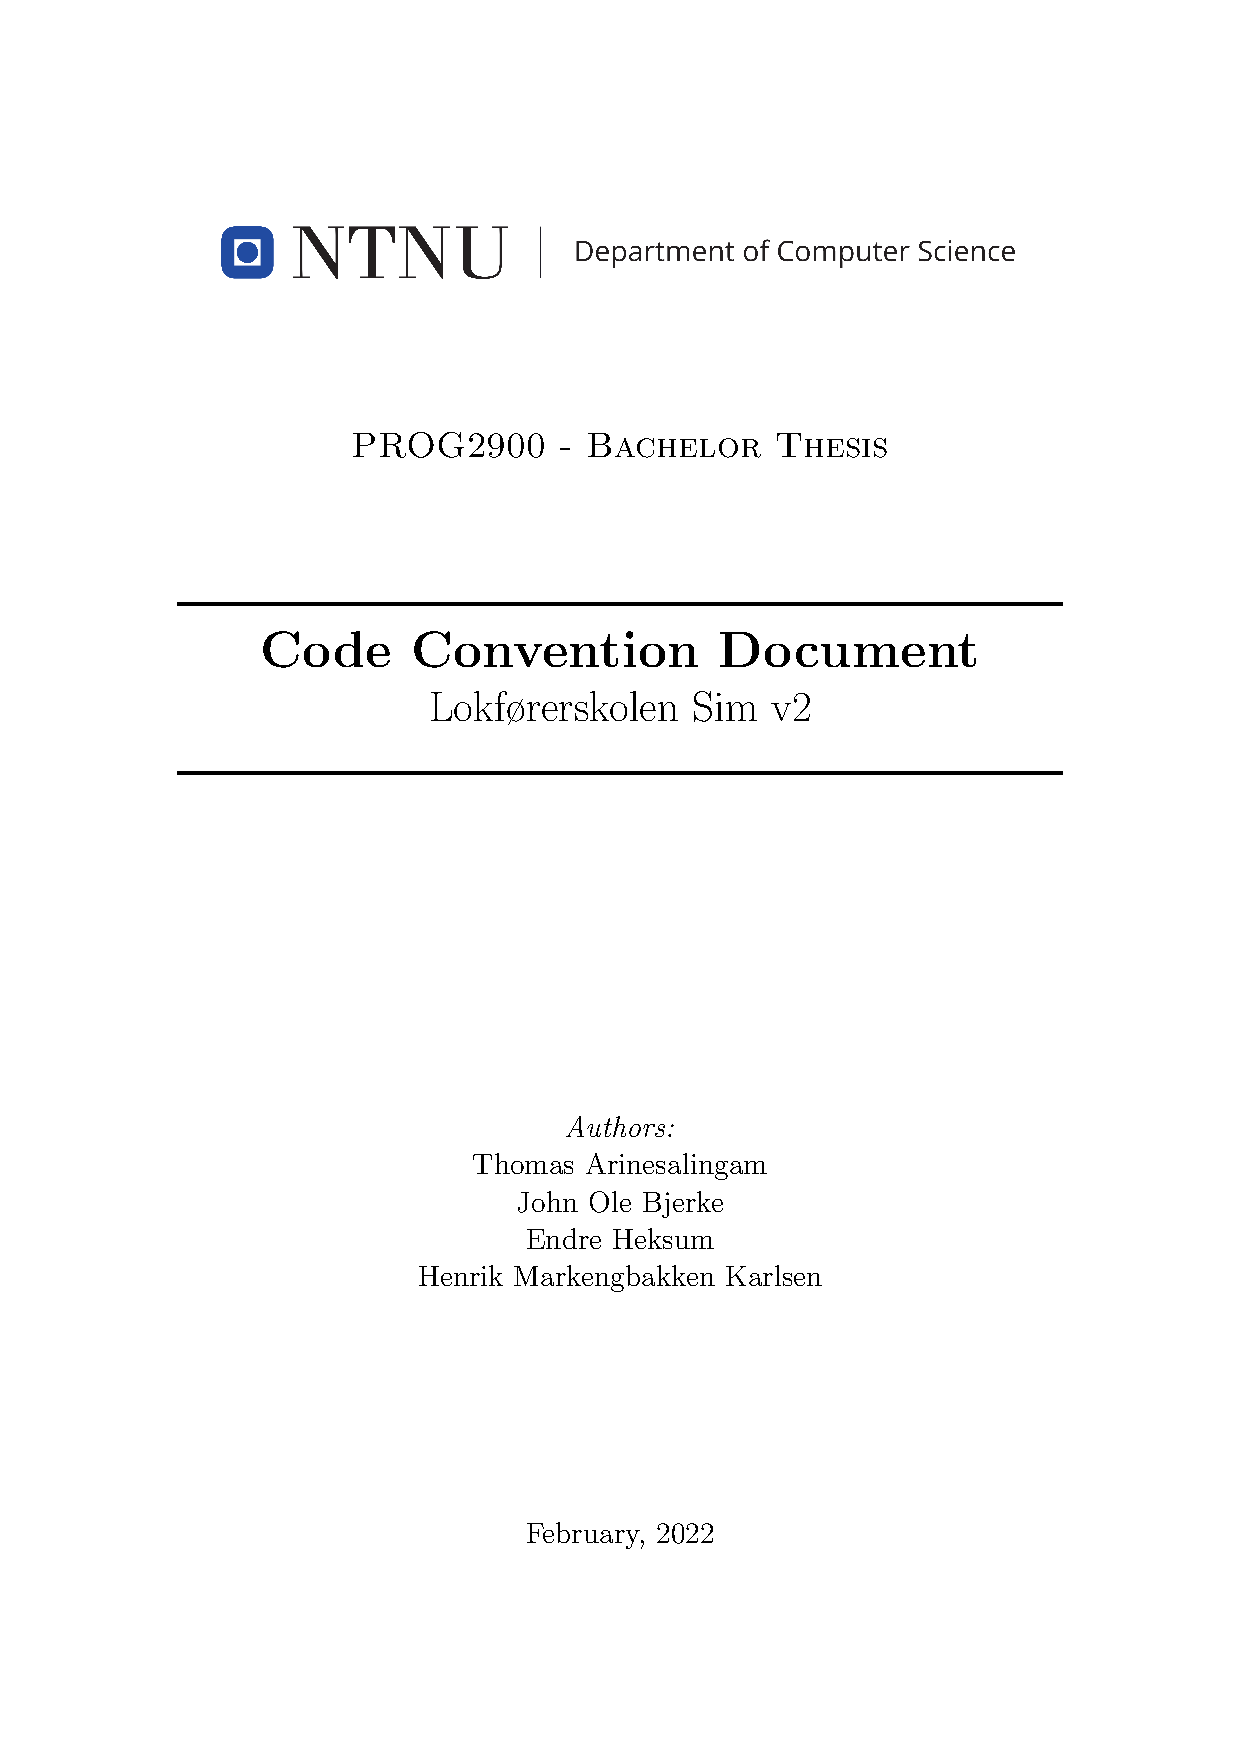
\includepdf[pages=-]{appendices/Code_Convention_Document.pdf}

\end{document}
